% Options for packages loaded elsewhere
\PassOptionsToPackage{unicode}{hyperref}
\PassOptionsToPackage{hyphens}{url}
%
\documentclass[
  10pt,
]{article}
\usepackage{amsmath,amssymb}
\usepackage{lmodern}
\usepackage{iftex}
\ifPDFTeX
  \usepackage[T1]{fontenc}
  \usepackage[utf8]{inputenc}
  \usepackage{textcomp} % provide euro and other symbols
\else % if luatex or xetex
  \usepackage{unicode-math}
  \defaultfontfeatures{Scale=MatchLowercase}
  \defaultfontfeatures[\rmfamily]{Ligatures=TeX,Scale=1}
  \setmainfont[]{Trebuchet MS}
  \setsansfont[]{Arial}
  \setmonofont[]{Menlo}
\fi
% Use upquote if available, for straight quotes in verbatim environments
\IfFileExists{upquote.sty}{\usepackage{upquote}}{}
\IfFileExists{microtype.sty}{% use microtype if available
  \usepackage[]{microtype}
  \UseMicrotypeSet[protrusion]{basicmath} % disable protrusion for tt fonts
}{}
\makeatletter
\@ifundefined{KOMAClassName}{% if non-KOMA class
  \IfFileExists{parskip.sty}{%
    \usepackage{parskip}
  }{% else
    \setlength{\parindent}{0pt}
    \setlength{\parskip}{6pt plus 2pt minus 1pt}}
}{% if KOMA class
  \KOMAoptions{parskip=half}}
\makeatother
\usepackage{xcolor}
\IfFileExists{xurl.sty}{\usepackage{xurl}}{} % add URL line breaks if available
\IfFileExists{bookmark.sty}{\usepackage{bookmark}}{\usepackage{hyperref}}
\hypersetup{
  pdftitle={Results of Statistical Analyses},
  hidelinks,
  pdfcreator={LaTeX via pandoc}}
\urlstyle{same} % disable monospaced font for URLs
\usepackage[margin=1in]{geometry}
\usepackage{graphicx}
\makeatletter
\def\maxwidth{\ifdim\Gin@nat@width>\linewidth\linewidth\else\Gin@nat@width\fi}
\def\maxheight{\ifdim\Gin@nat@height>\textheight\textheight\else\Gin@nat@height\fi}
\makeatother
% Scale images if necessary, so that they will not overflow the page
% margins by default, and it is still possible to overwrite the defaults
% using explicit options in \includegraphics[width, height, ...]{}
\setkeys{Gin}{width=\maxwidth,height=\maxheight,keepaspectratio}
% Set default figure placement to htbp
\makeatletter
\def\fps@figure{htbp}
\makeatother
\setlength{\emergencystretch}{3em} % prevent overfull lines
\providecommand{\tightlist}{%
  \setlength{\itemsep}{0pt}\setlength{\parskip}{0pt}}
\setcounter{secnumdepth}{-\maxdimen} % remove section numbering
\newlength{\cslhangindent}
\setlength{\cslhangindent}{1.5em}
\newlength{\csllabelwidth}
\setlength{\csllabelwidth}{3em}
\newlength{\cslentryspacingunit} % times entry-spacing
\setlength{\cslentryspacingunit}{\parskip}
\newenvironment{CSLReferences}[2] % #1 hanging-ident, #2 entry spacing
 {% don't indent paragraphs
  \setlength{\parindent}{0pt}
  % turn on hanging indent if param 1 is 1
  \ifodd #1
  \let\oldpar\par
  \def\par{\hangindent=\cslhangindent\oldpar}
  \fi
  % set entry spacing
  \setlength{\parskip}{#2\cslentryspacingunit}
 }%
 {}
\usepackage{calc}
\newcommand{\CSLBlock}[1]{#1\hfill\break}
\newcommand{\CSLLeftMargin}[1]{\parbox[t]{\csllabelwidth}{#1}}
\newcommand{\CSLRightInline}[1]{\parbox[t]{\linewidth - \csllabelwidth}{#1}\break}
\newcommand{\CSLIndent}[1]{\hspace{\cslhangindent}#1}
\usepackage{booktabs}
\usepackage{longtable}
\usepackage{tabularx}
\usepackage{array}
\usepackage{multirow}
\usepackage{wrapfig}
\usepackage{float}
\usepackage{colortbl}
\usepackage{pdflscape}
\usepackage{tabu}
\usepackage{threeparttable}
\usepackage{threeparttablex}
\usepackage[normalem]{ulem}
\usepackage{makecell}
\usepackage{xcolor}
\usepackage{amsmath}
\usepackage{setspace}\onehalfspacing
\usepackage{array}
\usepackage{caption}
\usepackage{graphicx}
\usepackage{siunitx}
\usepackage[normalem]{ulem}
\usepackage{colortbl}
\usepackage{multirow}
\usepackage{hhline}
\usepackage{calc}
\usepackage{tabularx}
\usepackage{threeparttable}
\usepackage{wrapfig}
\usepackage{adjustbox}
\usepackage{hyperref}
\usepackage{fontspec}
\ifLuaTeX
  \usepackage{selnolig}  % disable illegal ligatures
\fi

\title{Results of Statistical Analyses}
\usepackage{etoolbox}
\makeatletter
\providecommand{\subtitle}[1]{% add subtitle to \maketitle
  \apptocmd{\@title}{\par {\large #1 \par}}{}{}
}
\makeatother
\subtitle{Predictors of mortality of hospitalized patients with
laboratory-confirmed severe acute respiratory syndrome coronavirus 2 in
Nigeria: A retrospective analysis of high burden states}
\author{}
\date{\vspace{-2.5em}October 12, 2021}

\begin{document}
\maketitle

\newpage

\tableofcontents

\newpage

\listoftables

\newpage

\listoffigures

\newpage

\hypertarget{background}{%
\section{Background}\label{background}}

The current COVID 19 pandemic has resulted in a high number of deaths
and associated disruption of public health and socioeconomic activities
of countries and populations. As at 9th of April 2021, Nigeria had
recorded 163,581 confirmed cases, with 150,005 cases discharged, 7,518
cases on admission and 2,058 deaths with a significant increase in the
number of confirmed cases and concurrent deaths since the beginning of
the second wave of infections. Most of these deaths have been
in-hospital. Little is known about the deaths in the community due
largely to poor community records of deaths and other vital statistics.
The weak Nigerian health system is thought to have led to a considerably
high in-hospital mortality especially in settings where critical care
services and resources are scarce. Underlying morbidities such as
malnutrition, anemia, HIV/AIDs, and chronic respiratory conditions,
diabetes and heart failure have been shown to be important contributors
to high global mortality in the current COVID 19 pandemic.

Even though several global reports have been written about the impact of
the COVID 19 pandemic on clinical outcomes especially the attendant
morbidity and mortality, little is known about the situation in Nigeria.
Understanding the relative contributions and probable mechanism through
which sociodemographic, clinical and laboratory factors relate to the
high in-hospital mortality in Nigeria could help us identify weak points
within the health system that can be improved upon for current and
future responses. In addition, such review will also help us plan and
prioritize health infrastructure and resource allocation for better
health outcomes in our public health system.

The aim of this study was to describe clinical characteristics and
factors associated with mortality and time to mortality for patients
hospitalized with laboratory-confirmed severe acute respiratory syndrome
coronavirus 2 (SARS-CoV-2) infection in Nigeria.

\hypertarget{data-analysis-plan}{%
\section{Data Analysis Plan}\label{data-analysis-plan}}

\hypertarget{study-setting}{%
\subsection{Study Setting}\label{study-setting}}

Nigeria is Africa's most populous country. We studied patients with
laboratory-confirmed SARS-CoV-2 infection from 28 COVID 19 treatment
centers across 15 states in Nigeria including the Federal Capital
Territory (see Figure \ref{fig:states-map}).

\hypertarget{study-design}{%
\subsection{Study Design}\label{study-design}}

This study was a retrospective cross-sectional study.

\hypertarget{data-collection}{%
\subsection{Data Collection}\label{data-collection}}

\begin{figure}[h!]

{\centering 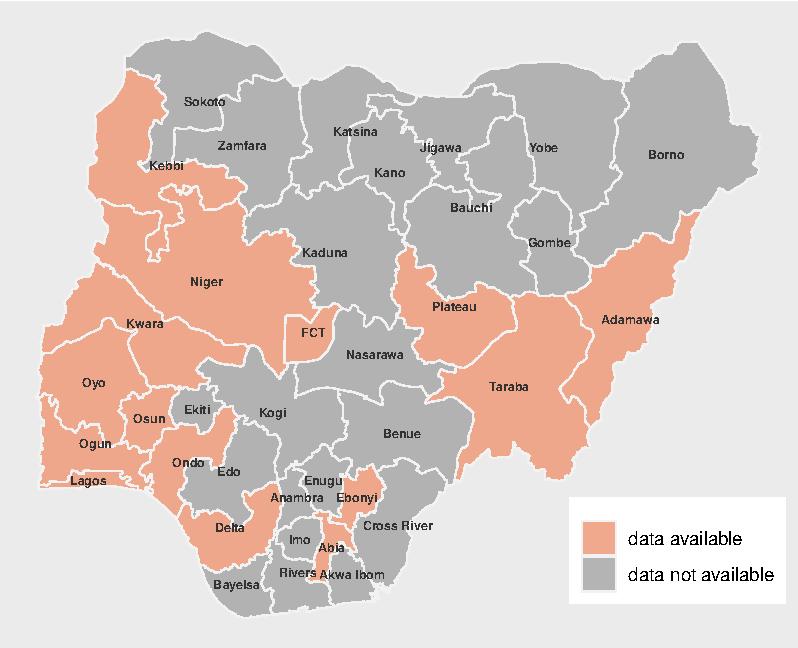
\includegraphics{results_files/figure-latex/states-map-1} 

}

\caption{States with available data}\label{fig:states-map}
\end{figure}

We extracted data from the World Health Organization (WHO) nCOV database
platform (OpenClinica Electronic Data Capture {[}EDC{]} System) for 28
sites across 15 states in Nigeria (see Figure \ref{fig:states-map}). We
retrieved data on date of admission, enrollment date, demographic data
(patients' sex, age, health worker), data on pre-existing morbidity
(chronic cardiac disease, hypertension, chronic pulmonary disease,
asthma, chronic kidney disease, chronic neurological disorder, HIV,
diabetes, current smoking, tuberculosis, asplenia, malignant neoplasm),
pre-admission and chronic medication (ACE inhibitors, angiotensin II
receptor blockers, non-steroidal anti-inflammatory drugs in the 14 days
prior to admission), medications received on day of admission or
following (antiviral, corticosteroid, chloroquine/hydroxychloroquine),
admitted to ICU or HDU, supplemental oxygen given, use of non-invasive
ventilation, use of invasive ventilation, outcome (discharged alive,
hospitalized, transfer to other facility, death, palliative discharge),
and outcome date. Following data cleaning, data recoding and removal of
missing observations we were left with 3,462 records for data analysis.
Two states (Delta and Taraba) were excluded because the states each had
less than 10 records: Delta (6), Taraba (1).

\hypertarget{study-variables}{%
\subsection{Study Variables}\label{study-variables}}

The primary study outcome was death for a PCR confirmed infection with
SARS-COV-2 virus. The secondary study outcome was time from enrollment
to death. We coded the primary study outcome as 1 if the patient died or
0 if outcome was censored. Time following admission was right-censored
at 84 days post-enrollment. The main explanatory variable was severity
of disease. We defined severity of disease as a composite score derived
from any or all of:

\begin{enumerate}
\def\labelenumi{\arabic{enumi}.}
\tightlist
\item
  Received supplemental oxygen therapy on any day during
  hospitalization,
\item
  Admitted to the ICU or HDU at any point during hospital stay,
\item
  Received non-invasive ventilation (CPAP/BIPAP) on any day during
  hospitalization, and
\item
  Received invasive ventilation (mechanical ventilator) on any day
  during hospitalization
\end{enumerate}

These variables were assigned a score of 1 if reported in the database
or 0, otherwise. The severity score was calculated as the sum of these
individual scores with a range of 0 to 4. The other explanatory
variables were demographic (age, sex, healthcare worker), pre-existing
morbidity (), malaria, HIV infection, pre-admission and chronic
medications, and medications received on admission or following
admission. These explanatory variables were coded as 1 if reported or 0
if not reported or missing.

\hypertarget{statistical-analysis}{%
\subsection{Statistical Analysis}\label{statistical-analysis}}

\hypertarget{power-calculation}{%
\subsubsection{Power calculation}\label{power-calculation}}

The relationship between the log odds of the mortality and \emph{k}
explanatory variables may be modeled thus:

\[{\small\log\Big(\frac{p}{1-p}\Big) = \beta_1x_1 + \beta_2x_2 + \cdots + \beta_kx_k}\]
The main explanatory covariate was severity score assumed to be normally
distributed based on the central limit theorem. Given two-sided testing
of \(H_0:\beta_i = 0\) on the log scale versus \(H_1:\beta_i \neq 0\)
the minimum sample size is then, according to Hsieh et
al.,\textsuperscript{\protect\hyperlink{ref-hsieh1998}{1}} given by:

\[\small{n = \frac{(z_{1-\alpha/2} + z_{\gamma})^2}{p(1 - p)(1-\rho^{2}_i)\hat{\beta}^2}}\]
with level \(\alpha\) and power \(\gamma\), the standard deviation of
the predictor \(x_i\) is \(\sigma_{x_i}\), \(p\) the marginal prevalence
of the outcome, \(\rho^{2}_i\) is the multiple correlation of \(x_i\)
with all the other predictors (i.e.~the \(R^2\)), \(z_{1-\alpha/2}\) and
\(z_\gamma\) are quantiles of the standard normal distribution
corresponding to level and power, \(\hat{\beta}^2\) is the effect size
(i.e.~the log odds ratio):

\[\hat{\beta} = \log\Bigg(\frac{p_1/1-p_1}{p_2/1-p_2}\Bigg)\] and
\(p_1\), \(p_2\) are the event rates at the mean of the severity score,
and one standard deviation above the mean severity score respectively.

Therefore the power is calculated as

\[\gamma = 1 - \Phi\Big(z_{1-\alpha/2} - |\hat{\beta}|\sqrt{np(1-p)(1-\rho^2_i)}\Big)\]
Where \(\Phi\) is the standard normal cumulative distribution function.

Using G*Power\textsuperscript{\protect\hyperlink{ref-faul2009}{2}} with
\(\alpha\) = 0.05, \(\hat{\beta}\) = 1.5, \(p\) = 0.05, \(R^2\) = 0.25
and assumed mean severity score of 2 with standard deviation of 1, we
determined that the number of subjects of 3,462 had greater than 95\%
power for a two-tailed hypothesis test (see Figure
\ref{fig:power-analysis}).

\begin{figure}[h]

{\centering 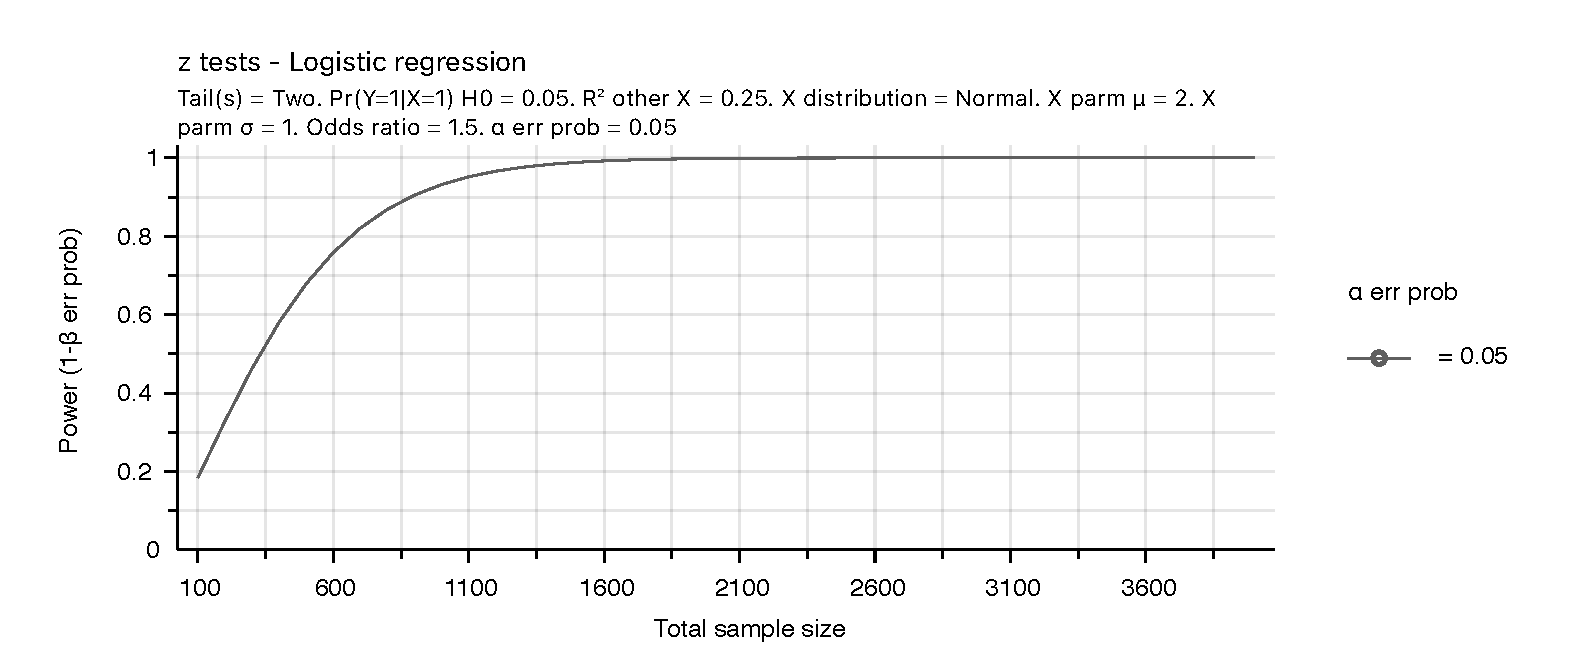
\includegraphics{power_plot} 

}

\caption{Plot of sample sizes versus power}\label{fig:power-analysis}
\end{figure}

\clearpage

\hypertarget{regression-modeling}{%
\subsubsection{Regression modeling}\label{regression-modeling}}

The term multilevel refers to individuals at a lower level who are
nested within spatial units at higher
levels.\textsuperscript{\protect\hyperlink{ref-subramanian2004}{3}}
Multilevel methods are suitable for the statistical analysis of data
with a nested structure. Multilevel regression modeling was used for the
data analysis in this study. These data were from several COVID-19
treatment sites across Nigeria (Figure \ref{fig:states-map}) with
clustering of patients by site. The sites in turn may be considered to
be nested by facility type e.g.~tertiary hospital, non-tertiary
hospital, and other treatment site.

Multilevel statistical modeling incorporates models at each level of
analysis into a full multilevel model. In general terms, for example, in
a two-level nested model, the model at the first level is expressed as

\[y_{ij} = \beta_{\textsf{0}j} + \beta_{1}x_{\textsf{1}ij} + e_{\textsf{0}ij}\]
Where \(y_{ij}\) is the measure of the dependent variable for the
\(i\)th individual in the \(j\)th group. The term
\(\beta_{\textsf{0}j}\) is a constant and is the measure of the
dependent variable for the jth group, and \(\beta_{1}\) is the fixed
marginal effect of the predictor variable (\(x_{\textsf{1}ij}\)) on the
dependent variable.

The individual or the level-1 residual term, \(e_{\textsf{0}ij}\), is
assumed to have a normal distribution with a mean of 0 and a variance,
\(\sigma^2_{e_{0}}\). In multilevel modeling, the coefficients at
level-1 become the outcome variables at level-2. Thus, the model at
level-2 can be written as

\[\beta_{\textsf{0}j} = \beta_{0} + u_{\textsf{0}j}\]

meaning the mean measure of the dependent variable for the \(j\)th group
is split into \(\beta_{0}\) (the average for the dependent variable
across all groups), and \(u_{\textsf{0}j}\), the effect specific to the
\(j\)th group, and \(u_{\textsf{0}j}\) can be treated similar to
individual-level residuals. Combining the two equations above yields the
full model. This full model is known as a random-intercepts or variance
components model:

\[y_{ij} = \beta_{0} + \beta_{1}x_{\textsf{1}ij} + (u_{\textsf{0}j} + e_{\textsf{0}ij})\]

In this multilevel statistical model, the variance at level-2,
\(\sigma^2_{u_{0}}\), measures the group differences after accounting
for the compositional effect of the predictor variable and thus
separates the effects of the individual-level variables from the
contextual differences between group-level
variables.\textsuperscript{\protect\hyperlink{ref-subramanian2004}{3}}
Therefore using multilevel modeling we can (a) model the variation in
patient-level regression coefficients across sites, (b) account for the
patient- and site-level variation in estimating site-level coefficients,
and (c) estimate regression coefficients for particular
groups.\textsuperscript{\protect\hyperlink{ref-gelman2007}{4}}

We performed univariate analysis using the Fisher exact test, or the
Wilcoxon test as appropriate to describe characteristics of patients who
had non-missing outcome data (see Table \ref{tab:table-1}). We also did
univariate survival analysis using the Kaplan-Meier method to assess the
relationship between time from enrollment to death and patient
characteristics. We further fitted mixed effects logistic regression
models and Cox proportional hazards regression models to assess
predictors of COVID-19 hospital death. Study site and facility type were
included in the models as random effects while severity score, patients'
sex, age, health worker status, chronic cardiac disease, hypertension,
respiratory disease (any of chronic pulmonary disease, active or
previous tuberculosis, asthma), chronic kidney disease, chronic
neurological disorder, HIV, diabetes, current smoking, malignant
neoplasm, malaria, pre-admission and chronic medication (ACE inhibitors,
angiotensin II receptor blockers, non-steroidal anti-inflammatory drugs
in the 14 days prior to admission), medications received on day of
admission or following admission (antiviral, corticosteroid,
azithromycin, chloroquine/hydroxychloroquine) were included as fixed
effects. We report the models with the smallest AIC selected by stepwise
regression. All statistical analysis were conducted using R version
4.1.1.\textsuperscript{\protect\hyperlink{ref-rcoreteam2021}{5}} Mixed
effects Cox regression was done using the \texttt{coxme}
package.\textsuperscript{\protect\hyperlink{ref-therneau2020}{6}}. A p
value \textless{} 0.05 is considered as statistically significant.

\newpage

\hypertarget{results}{%
\section{Results}\label{results}}

\hypertarget{patient-characteristics}{%
\subsection{Patient characteristics}\label{patient-characteristics}}

 
  \providecommand{\huxb}[2]{\arrayrulecolor[RGB]{#1}\global\arrayrulewidth=#2pt}
  \providecommand{\huxvb}[2]{\color[RGB]{#1}\vrule width #2pt}
  \providecommand{\huxtpad}[1]{\rule{0pt}{#1}}
  \providecommand{\huxbpad}[1]{\rule[-#1]{0pt}{#1}}

\begin{table}[h!]
\begin{centerbox}
\begin{threeparttable}
\captionsetup{justification=centering,singlelinecheck=off}
\caption{Patient characteristics}
 \label{tab:table-1}
\setlength{\tabcolsep}{0pt}
\begin{tabularx}{0.96\textwidth}{p{0.48\textwidth} p{0.192\textwidth} p{0.192\textwidth} p{0.096\textwidth}}


\hhline{>{\huxb{0, 0, 0}{0.4}}->{\huxb{0, 0, 0}{0.4}}->{\huxb{0, 0, 0}{0.4}}->{\huxb{0, 0, 0}{0.4}}-}
\arrayrulecolor{black}

\multicolumn{1}{!{\huxvb{0, 0, 0}{0}}p{0.48\textwidth}!{\huxvb{0, 0, 0}{0}}}{\cellcolor[RGB]{255, 255, 255}\hspace{6pt}\parbox[b]{0.48\textwidth-6pt-6pt}{\huxtpad{1pt + 1em}\raggedright {\fontsize{8pt}{9.6pt}\selectfont 
}\huxbpad{1pt}}} &
\multicolumn{2}{p{0.384\textwidth+2\tabcolsep}!{\huxvb{0, 0, 0}{0}}}{\cellcolor[RGB]{255, 255, 255}\hspace{6pt}\parbox[b]{0.384\textwidth+2\tabcolsep-6pt-6pt}{\huxtpad{1pt + 1em}\centering {\fontsize{8pt}{9.6pt}\selectfont \textbf{Died}
}\huxbpad{1pt}}} &
\multicolumn{1}{p{0.096\textwidth}!{\huxvb{0, 0, 0}{0}}}{\cellcolor[RGB]{255, 255, 255}\hspace{6pt}\parbox[b]{0.096\textwidth-6pt-6pt}{\huxtpad{1pt + 1em}\raggedleft {\fontsize{8pt}{9.6pt}\selectfont 
}\huxbpad{1pt}}} \tabularnewline[-0.5pt]


\hhline{>{\huxb{255, 255, 255}{0.4}}->{\huxb{0, 0, 0}{0.4}}->{\huxb{0, 0, 0}{0.4}}->{\huxb{255, 255, 255}{0.4}}-}
\arrayrulecolor{black}

\multicolumn{1}{!{\huxvb{0, 0, 0}{0}}p{0.48\textwidth}!{\huxvb{0, 0, 0}{0}}}{\cellcolor[RGB]{255, 255, 255}\hspace{6pt}\parbox[b]{0.48\textwidth-6pt-6pt}{\huxtpad{1pt + 1em}\raggedright {\fontsize{8pt}{9.6pt}\selectfont \textbf{Variables}
}\huxbpad{1pt}}} &
\multicolumn{1}{p{0.192\textwidth}!{\huxvb{0, 0, 0}{0}}}{\cellcolor[RGB]{255, 255, 255}\hspace{6pt}\parbox[b]{0.192\textwidth-6pt-6pt}{\huxtpad{1pt + 1em}\centering {\fontsize{8pt}{9.6pt}\selectfont \textbf{No},  \emph{N} = 3,249
}\huxbpad{1pt}}} &
\multicolumn{1}{p{0.192\textwidth}!{\huxvb{0, 0, 0}{0}}}{\cellcolor[RGB]{255, 255, 255}\hspace{6pt}\parbox[b]{0.192\textwidth-6pt-6pt}{\huxtpad{1pt + 1em}\centering {\fontsize{8pt}{9.6pt}\selectfont \textbf{Yes}, \emph{N} = 213
}\huxbpad{1pt}}} &
\multicolumn{1}{p{0.096\textwidth}!{\huxvb{0, 0, 0}{0}}}{\cellcolor[RGB]{255, 255, 255}\hspace{6pt}\parbox[b]{0.096\textwidth-6pt-6pt}{\huxtpad{1pt + 1em}\raggedleft {\fontsize{8pt}{9.6pt}\selectfont \textbf{p value}
}\huxbpad{1pt}}} \tabularnewline[-0.5pt]


\hhline{>{\huxb{0, 0, 0}{0.4}}->{\huxb{0, 0, 0}{0.4}}->{\huxb{0, 0, 0}{0.4}}->{\huxb{0, 0, 0}{0.4}}-}
\arrayrulecolor{black}

\multicolumn{1}{!{\huxvb{0, 0, 0}{0}}p{0.48\textwidth}!{\huxvb{0, 0, 0}{0}}}{\cellcolor[RGB]{255, 255, 255}\hspace{6pt}\parbox[b]{0.48\textwidth-6pt-6pt}{\huxtpad{1pt + 1em}\raggedright {\fontsize{8pt}{9.6pt}\selectfont Severity score}\huxbpad{1pt}}} &
\multicolumn{1}{p{0.192\textwidth}!{\huxvb{0, 0, 0}{0}}}{\cellcolor[RGB]{255, 255, 255}\hspace{6pt}\parbox[b]{0.192\textwidth-6pt-6pt}{\huxtpad{1pt + 1em}\centering {\fontsize{8pt}{9.6pt}\selectfont }\huxbpad{1pt}}} &
\multicolumn{1}{p{0.192\textwidth}!{\huxvb{0, 0, 0}{0}}}{\cellcolor[RGB]{255, 255, 255}\hspace{6pt}\parbox[b]{0.192\textwidth-6pt-6pt}{\huxtpad{1pt + 1em}\centering {\fontsize{8pt}{9.6pt}\selectfont }\huxbpad{1pt}}} &
\multicolumn{1}{p{0.096\textwidth}!{\huxvb{0, 0, 0}{0}}}{\cellcolor[RGB]{255, 255, 255}\hspace{6pt}\parbox[b]{0.096\textwidth-6pt-6pt}{\huxtpad{1pt + 1em}\raggedleft \textbf{{\fontsize{8pt}{9.6pt}\selectfont $<$0.001}}\huxbpad{1pt}}} \tabularnewline[-0.5pt]


\hhline{}
\arrayrulecolor{black}

\multicolumn{1}{!{\huxvb{0, 0, 0}{0}}p{0.48\textwidth}!{\huxvb{0, 0, 0}{0}}}{\cellcolor[RGB]{240, 240, 240}\hspace{15pt}\parbox[b]{0.48\textwidth-15pt-6pt}{\huxtpad{1pt + 1em}\raggedright {\fontsize{8pt}{9.6pt}\selectfont 0}\huxbpad{1pt}}} &
\multicolumn{1}{p{0.192\textwidth}!{\huxvb{0, 0, 0}{0}}}{\cellcolor[RGB]{240, 240, 240}\hspace{6pt}\parbox[b]{0.192\textwidth-6pt-6pt}{\huxtpad{1pt + 1em}\centering {\fontsize{8pt}{9.6pt}\selectfont 2,916 (89.8\%)}\huxbpad{1pt}}} &
\multicolumn{1}{p{0.192\textwidth}!{\huxvb{0, 0, 0}{0}}}{\cellcolor[RGB]{240, 240, 240}\hspace{6pt}\parbox[b]{0.192\textwidth-6pt-6pt}{\huxtpad{1pt + 1em}\centering {\fontsize{8pt}{9.6pt}\selectfont 89 (41.8\%)}\huxbpad{1pt}}} &
\multicolumn{1}{p{0.096\textwidth}!{\huxvb{0, 0, 0}{0}}}{\cellcolor[RGB]{240, 240, 240}\hspace{6pt}\parbox[b]{0.096\textwidth-6pt-6pt}{\huxtpad{1pt + 1em}\raggedleft {\fontsize{8pt}{9.6pt}\selectfont }\huxbpad{1pt}}} \tabularnewline[-0.5pt]


\hhline{}
\arrayrulecolor{black}

\multicolumn{1}{!{\huxvb{0, 0, 0}{0}}p{0.48\textwidth}!{\huxvb{0, 0, 0}{0}}}{\cellcolor[RGB]{255, 255, 255}\hspace{15pt}\parbox[b]{0.48\textwidth-15pt-6pt}{\huxtpad{1pt + 1em}\raggedright {\fontsize{8pt}{9.6pt}\selectfont 1}\huxbpad{1pt}}} &
\multicolumn{1}{p{0.192\textwidth}!{\huxvb{0, 0, 0}{0}}}{\cellcolor[RGB]{255, 255, 255}\hspace{6pt}\parbox[b]{0.192\textwidth-6pt-6pt}{\huxtpad{1pt + 1em}\centering {\fontsize{8pt}{9.6pt}\selectfont 249 (7.7\%)}\huxbpad{1pt}}} &
\multicolumn{1}{p{0.192\textwidth}!{\huxvb{0, 0, 0}{0}}}{\cellcolor[RGB]{255, 255, 255}\hspace{6pt}\parbox[b]{0.192\textwidth-6pt-6pt}{\huxtpad{1pt + 1em}\centering {\fontsize{8pt}{9.6pt}\selectfont 71 (33.3\%)}\huxbpad{1pt}}} &
\multicolumn{1}{p{0.096\textwidth}!{\huxvb{0, 0, 0}{0}}}{\cellcolor[RGB]{255, 255, 255}\hspace{6pt}\parbox[b]{0.096\textwidth-6pt-6pt}{\huxtpad{1pt + 1em}\raggedleft {\fontsize{8pt}{9.6pt}\selectfont }\huxbpad{1pt}}} \tabularnewline[-0.5pt]


\hhline{}
\arrayrulecolor{black}

\multicolumn{1}{!{\huxvb{0, 0, 0}{0}}p{0.48\textwidth}!{\huxvb{0, 0, 0}{0}}}{\cellcolor[RGB]{240, 240, 240}\hspace{15pt}\parbox[b]{0.48\textwidth-15pt-6pt}{\huxtpad{1pt + 1em}\raggedright {\fontsize{8pt}{9.6pt}\selectfont 2}\huxbpad{1pt}}} &
\multicolumn{1}{p{0.192\textwidth}!{\huxvb{0, 0, 0}{0}}}{\cellcolor[RGB]{240, 240, 240}\hspace{6pt}\parbox[b]{0.192\textwidth-6pt-6pt}{\huxtpad{1pt + 1em}\centering {\fontsize{8pt}{9.6pt}\selectfont 78 (2.4\%)}\huxbpad{1pt}}} &
\multicolumn{1}{p{0.192\textwidth}!{\huxvb{0, 0, 0}{0}}}{\cellcolor[RGB]{240, 240, 240}\hspace{6pt}\parbox[b]{0.192\textwidth-6pt-6pt}{\huxtpad{1pt + 1em}\centering {\fontsize{8pt}{9.6pt}\selectfont 47 (22.1\%)}\huxbpad{1pt}}} &
\multicolumn{1}{p{0.096\textwidth}!{\huxvb{0, 0, 0}{0}}}{\cellcolor[RGB]{240, 240, 240}\hspace{6pt}\parbox[b]{0.096\textwidth-6pt-6pt}{\huxtpad{1pt + 1em}\raggedleft {\fontsize{8pt}{9.6pt}\selectfont }\huxbpad{1pt}}} \tabularnewline[-0.5pt]


\hhline{}
\arrayrulecolor{black}

\multicolumn{1}{!{\huxvb{0, 0, 0}{0}}p{0.48\textwidth}!{\huxvb{0, 0, 0}{0}}}{\cellcolor[RGB]{255, 255, 255}\hspace{15pt}\parbox[b]{0.48\textwidth-15pt-6pt}{\huxtpad{1pt + 1em}\raggedright {\fontsize{8pt}{9.6pt}\selectfont 3}\huxbpad{1pt}}} &
\multicolumn{1}{p{0.192\textwidth}!{\huxvb{0, 0, 0}{0}}}{\cellcolor[RGB]{255, 255, 255}\hspace{6pt}\parbox[b]{0.192\textwidth-6pt-6pt}{\huxtpad{1pt + 1em}\centering {\fontsize{8pt}{9.6pt}\selectfont 5 (0.2\%)}\huxbpad{1pt}}} &
\multicolumn{1}{p{0.192\textwidth}!{\huxvb{0, 0, 0}{0}}}{\cellcolor[RGB]{255, 255, 255}\hspace{6pt}\parbox[b]{0.192\textwidth-6pt-6pt}{\huxtpad{1pt + 1em}\centering {\fontsize{8pt}{9.6pt}\selectfont 5 (2.3\%)}\huxbpad{1pt}}} &
\multicolumn{1}{p{0.096\textwidth}!{\huxvb{0, 0, 0}{0}}}{\cellcolor[RGB]{255, 255, 255}\hspace{6pt}\parbox[b]{0.096\textwidth-6pt-6pt}{\huxtpad{1pt + 1em}\raggedleft {\fontsize{8pt}{9.6pt}\selectfont }\huxbpad{1pt}}} \tabularnewline[-0.5pt]


\hhline{}
\arrayrulecolor{black}

\multicolumn{1}{!{\huxvb{0, 0, 0}{0}}p{0.48\textwidth}!{\huxvb{0, 0, 0}{0}}}{\cellcolor[RGB]{240, 240, 240}\hspace{15pt}\parbox[b]{0.48\textwidth-15pt-6pt}{\huxtpad{1pt + 1em}\raggedright {\fontsize{8pt}{9.6pt}\selectfont 4}\huxbpad{1pt}}} &
\multicolumn{1}{p{0.192\textwidth}!{\huxvb{0, 0, 0}{0}}}{\cellcolor[RGB]{240, 240, 240}\hspace{6pt}\parbox[b]{0.192\textwidth-6pt-6pt}{\huxtpad{1pt + 1em}\centering {\fontsize{8pt}{9.6pt}\selectfont 1 (0\%)}\huxbpad{1pt}}} &
\multicolumn{1}{p{0.192\textwidth}!{\huxvb{0, 0, 0}{0}}}{\cellcolor[RGB]{240, 240, 240}\hspace{6pt}\parbox[b]{0.192\textwidth-6pt-6pt}{\huxtpad{1pt + 1em}\centering {\fontsize{8pt}{9.6pt}\selectfont 1 (0.5\%)}\huxbpad{1pt}}} &
\multicolumn{1}{p{0.096\textwidth}!{\huxvb{0, 0, 0}{0}}}{\cellcolor[RGB]{240, 240, 240}\hspace{6pt}\parbox[b]{0.096\textwidth-6pt-6pt}{\huxtpad{1pt + 1em}\raggedleft {\fontsize{8pt}{9.6pt}\selectfont }\huxbpad{1pt}}} \tabularnewline[-0.5pt]


\hhline{}
\arrayrulecolor{black}

\multicolumn{1}{!{\huxvb{0, 0, 0}{0}}p{0.48\textwidth}!{\huxvb{0, 0, 0}{0}}}{\cellcolor[RGB]{255, 255, 255}\hspace{6pt}\parbox[b]{0.48\textwidth-6pt-6pt}{\huxtpad{1pt + 1em}\raggedright {\fontsize{8pt}{9.6pt}\selectfont Days from enrollment to outcome, Median (IQR)}\huxbpad{1pt}}} &
\multicolumn{1}{p{0.192\textwidth}!{\huxvb{0, 0, 0}{0}}}{\cellcolor[RGB]{255, 255, 255}\hspace{6pt}\parbox[b]{0.192\textwidth-6pt-6pt}{\huxtpad{1pt + 1em}\centering {\fontsize{8pt}{9.6pt}\selectfont 12 (7, 15)}\huxbpad{1pt}}} &
\multicolumn{1}{p{0.192\textwidth}!{\huxvb{0, 0, 0}{0}}}{\cellcolor[RGB]{255, 255, 255}\hspace{6pt}\parbox[b]{0.192\textwidth-6pt-6pt}{\huxtpad{1pt + 1em}\centering {\fontsize{8pt}{9.6pt}\selectfont 2 (1, 10)}\huxbpad{1pt}}} &
\multicolumn{1}{p{0.096\textwidth}!{\huxvb{0, 0, 0}{0}}}{\cellcolor[RGB]{255, 255, 255}\hspace{6pt}\parbox[b]{0.096\textwidth-6pt-6pt}{\huxtpad{1pt + 1em}\raggedleft \textbf{{\fontsize{8pt}{9.6pt}\selectfont $<$0.001}}\huxbpad{1pt}}} \tabularnewline[-0.5pt]


\hhline{}
\arrayrulecolor{black}

\multicolumn{1}{!{\huxvb{0, 0, 0}{0}}p{0.48\textwidth}!{\huxvb{0, 0, 0}{0}}}{\cellcolor[RGB]{240, 240, 240}\hspace{6pt}\parbox[b]{0.48\textwidth-6pt-6pt}{\huxtpad{1pt + 1em}\raggedright {\fontsize{8pt}{9.6pt}\selectfont Age, Median (IQR)}\huxbpad{1pt}}} &
\multicolumn{1}{p{0.192\textwidth}!{\huxvb{0, 0, 0}{0}}}{\cellcolor[RGB]{240, 240, 240}\hspace{6pt}\parbox[b]{0.192\textwidth-6pt-6pt}{\huxtpad{1pt + 1em}\centering {\fontsize{8pt}{9.6pt}\selectfont 39 (28, 53)}\huxbpad{1pt}}} &
\multicolumn{1}{p{0.192\textwidth}!{\huxvb{0, 0, 0}{0}}}{\cellcolor[RGB]{240, 240, 240}\hspace{6pt}\parbox[b]{0.192\textwidth-6pt-6pt}{\huxtpad{1pt + 1em}\centering {\fontsize{8pt}{9.6pt}\selectfont 61 (48, 70)}\huxbpad{1pt}}} &
\multicolumn{1}{p{0.096\textwidth}!{\huxvb{0, 0, 0}{0}}}{\cellcolor[RGB]{240, 240, 240}\hspace{6pt}\parbox[b]{0.096\textwidth-6pt-6pt}{\huxtpad{1pt + 1em}\raggedleft \textbf{{\fontsize{8pt}{9.6pt}\selectfont $<$0.001}}\huxbpad{1pt}}} \tabularnewline[-0.5pt]


\hhline{}
\arrayrulecolor{black}

\multicolumn{1}{!{\huxvb{0, 0, 0}{0}}p{0.48\textwidth}!{\huxvb{0, 0, 0}{0}}}{\cellcolor[RGB]{255, 255, 255}\hspace{6pt}\parbox[b]{0.48\textwidth-6pt-6pt}{\huxtpad{1pt + 1em}\raggedright {\fontsize{8pt}{9.6pt}\selectfont Age group}\huxbpad{1pt}}} &
\multicolumn{1}{p{0.192\textwidth}!{\huxvb{0, 0, 0}{0}}}{\cellcolor[RGB]{255, 255, 255}\hspace{6pt}\parbox[b]{0.192\textwidth-6pt-6pt}{\huxtpad{1pt + 1em}\centering {\fontsize{8pt}{9.6pt}\selectfont }\huxbpad{1pt}}} &
\multicolumn{1}{p{0.192\textwidth}!{\huxvb{0, 0, 0}{0}}}{\cellcolor[RGB]{255, 255, 255}\hspace{6pt}\parbox[b]{0.192\textwidth-6pt-6pt}{\huxtpad{1pt + 1em}\centering {\fontsize{8pt}{9.6pt}\selectfont }\huxbpad{1pt}}} &
\multicolumn{1}{p{0.096\textwidth}!{\huxvb{0, 0, 0}{0}}}{\cellcolor[RGB]{255, 255, 255}\hspace{6pt}\parbox[b]{0.096\textwidth-6pt-6pt}{\huxtpad{1pt + 1em}\raggedleft \textbf{{\fontsize{8pt}{9.6pt}\selectfont $<$0.001}}\huxbpad{1pt}}} \tabularnewline[-0.5pt]


\hhline{}
\arrayrulecolor{black}

\multicolumn{1}{!{\huxvb{0, 0, 0}{0}}p{0.48\textwidth}!{\huxvb{0, 0, 0}{0}}}{\cellcolor[RGB]{240, 240, 240}\hspace{15pt}\parbox[b]{0.48\textwidth-15pt-6pt}{\huxtpad{1pt + 1em}\raggedright {\fontsize{8pt}{9.6pt}\selectfont $<$18}\huxbpad{1pt}}} &
\multicolumn{1}{p{0.192\textwidth}!{\huxvb{0, 0, 0}{0}}}{\cellcolor[RGB]{240, 240, 240}\hspace{6pt}\parbox[b]{0.192\textwidth-6pt-6pt}{\huxtpad{1pt + 1em}\centering {\fontsize{8pt}{9.6pt}\selectfont 252 (8.1\%)}\huxbpad{1pt}}} &
\multicolumn{1}{p{0.192\textwidth}!{\huxvb{0, 0, 0}{0}}}{\cellcolor[RGB]{240, 240, 240}\hspace{6pt}\parbox[b]{0.192\textwidth-6pt-6pt}{\huxtpad{1pt + 1em}\centering {\fontsize{8pt}{9.6pt}\selectfont 4 (1.9\%)}\huxbpad{1pt}}} &
\multicolumn{1}{p{0.096\textwidth}!{\huxvb{0, 0, 0}{0}}}{\cellcolor[RGB]{240, 240, 240}\hspace{6pt}\parbox[b]{0.096\textwidth-6pt-6pt}{\huxtpad{1pt + 1em}\raggedleft {\fontsize{8pt}{9.6pt}\selectfont }\huxbpad{1pt}}} \tabularnewline[-0.5pt]


\hhline{}
\arrayrulecolor{black}

\multicolumn{1}{!{\huxvb{0, 0, 0}{0}}p{0.48\textwidth}!{\huxvb{0, 0, 0}{0}}}{\cellcolor[RGB]{255, 255, 255}\hspace{15pt}\parbox[b]{0.48\textwidth-15pt-6pt}{\huxtpad{1pt + 1em}\raggedright {\fontsize{8pt}{9.6pt}\selectfont 18$-$45}\huxbpad{1pt}}} &
\multicolumn{1}{p{0.192\textwidth}!{\huxvb{0, 0, 0}{0}}}{\cellcolor[RGB]{255, 255, 255}\hspace{6pt}\parbox[b]{0.192\textwidth-6pt-6pt}{\huxtpad{1pt + 1em}\centering {\fontsize{8pt}{9.6pt}\selectfont 1,688 (54.4\%)}\huxbpad{1pt}}} &
\multicolumn{1}{p{0.192\textwidth}!{\huxvb{0, 0, 0}{0}}}{\cellcolor[RGB]{255, 255, 255}\hspace{6pt}\parbox[b]{0.192\textwidth-6pt-6pt}{\huxtpad{1pt + 1em}\centering {\fontsize{8pt}{9.6pt}\selectfont 39 (18.7\%)}\huxbpad{1pt}}} &
\multicolumn{1}{p{0.096\textwidth}!{\huxvb{0, 0, 0}{0}}}{\cellcolor[RGB]{255, 255, 255}\hspace{6pt}\parbox[b]{0.096\textwidth-6pt-6pt}{\huxtpad{1pt + 1em}\raggedleft {\fontsize{8pt}{9.6pt}\selectfont }\huxbpad{1pt}}} \tabularnewline[-0.5pt]


\hhline{}
\arrayrulecolor{black}

\multicolumn{1}{!{\huxvb{0, 0, 0}{0}}p{0.48\textwidth}!{\huxvb{0, 0, 0}{0}}}{\cellcolor[RGB]{240, 240, 240}\hspace{15pt}\parbox[b]{0.48\textwidth-15pt-6pt}{\huxtpad{1pt + 1em}\raggedright {\fontsize{8pt}{9.6pt}\selectfont 46$-$65}\huxbpad{1pt}}} &
\multicolumn{1}{p{0.192\textwidth}!{\huxvb{0, 0, 0}{0}}}{\cellcolor[RGB]{240, 240, 240}\hspace{6pt}\parbox[b]{0.192\textwidth-6pt-6pt}{\huxtpad{1pt + 1em}\centering {\fontsize{8pt}{9.6pt}\selectfont 894 (28.8\%)}\huxbpad{1pt}}} &
\multicolumn{1}{p{0.192\textwidth}!{\huxvb{0, 0, 0}{0}}}{\cellcolor[RGB]{240, 240, 240}\hspace{6pt}\parbox[b]{0.192\textwidth-6pt-6pt}{\huxtpad{1pt + 1em}\centering {\fontsize{8pt}{9.6pt}\selectfont 95 (45.5\%)}\huxbpad{1pt}}} &
\multicolumn{1}{p{0.096\textwidth}!{\huxvb{0, 0, 0}{0}}}{\cellcolor[RGB]{240, 240, 240}\hspace{6pt}\parbox[b]{0.096\textwidth-6pt-6pt}{\huxtpad{1pt + 1em}\raggedleft {\fontsize{8pt}{9.6pt}\selectfont }\huxbpad{1pt}}} \tabularnewline[-0.5pt]


\hhline{}
\arrayrulecolor{black}

\multicolumn{1}{!{\huxvb{0, 0, 0}{0}}p{0.48\textwidth}!{\huxvb{0, 0, 0}{0}}}{\cellcolor[RGB]{255, 255, 255}\hspace{15pt}\parbox[b]{0.48\textwidth-15pt-6pt}{\huxtpad{1pt + 1em}\raggedright {\fontsize{8pt}{9.6pt}\selectfont 66$-$75}\huxbpad{1pt}}} &
\multicolumn{1}{p{0.192\textwidth}!{\huxvb{0, 0, 0}{0}}}{\cellcolor[RGB]{255, 255, 255}\hspace{6pt}\parbox[b]{0.192\textwidth-6pt-6pt}{\huxtpad{1pt + 1em}\centering {\fontsize{8pt}{9.6pt}\selectfont 183 (5.9\%)}\huxbpad{1pt}}} &
\multicolumn{1}{p{0.192\textwidth}!{\huxvb{0, 0, 0}{0}}}{\cellcolor[RGB]{255, 255, 255}\hspace{6pt}\parbox[b]{0.192\textwidth-6pt-6pt}{\huxtpad{1pt + 1em}\centering {\fontsize{8pt}{9.6pt}\selectfont 41 (19.6\%)}\huxbpad{1pt}}} &
\multicolumn{1}{p{0.096\textwidth}!{\huxvb{0, 0, 0}{0}}}{\cellcolor[RGB]{255, 255, 255}\hspace{6pt}\parbox[b]{0.096\textwidth-6pt-6pt}{\huxtpad{1pt + 1em}\raggedleft {\fontsize{8pt}{9.6pt}\selectfont }\huxbpad{1pt}}} \tabularnewline[-0.5pt]


\hhline{}
\arrayrulecolor{black}

\multicolumn{1}{!{\huxvb{0, 0, 0}{0}}p{0.48\textwidth}!{\huxvb{0, 0, 0}{0}}}{\cellcolor[RGB]{240, 240, 240}\hspace{15pt}\parbox[b]{0.48\textwidth-15pt-6pt}{\huxtpad{1pt + 1em}\raggedright {\fontsize{8pt}{9.6pt}\selectfont $>$75}\huxbpad{1pt}}} &
\multicolumn{1}{p{0.192\textwidth}!{\huxvb{0, 0, 0}{0}}}{\cellcolor[RGB]{240, 240, 240}\hspace{6pt}\parbox[b]{0.192\textwidth-6pt-6pt}{\huxtpad{1pt + 1em}\centering {\fontsize{8pt}{9.6pt}\selectfont 87 (2.8\%)}\huxbpad{1pt}}} &
\multicolumn{1}{p{0.192\textwidth}!{\huxvb{0, 0, 0}{0}}}{\cellcolor[RGB]{240, 240, 240}\hspace{6pt}\parbox[b]{0.192\textwidth-6pt-6pt}{\huxtpad{1pt + 1em}\centering {\fontsize{8pt}{9.6pt}\selectfont 30 (14.4\%)}\huxbpad{1pt}}} &
\multicolumn{1}{p{0.096\textwidth}!{\huxvb{0, 0, 0}{0}}}{\cellcolor[RGB]{240, 240, 240}\hspace{6pt}\parbox[b]{0.096\textwidth-6pt-6pt}{\huxtpad{1pt + 1em}\raggedleft {\fontsize{8pt}{9.6pt}\selectfont }\huxbpad{1pt}}} \tabularnewline[-0.5pt]


\hhline{}
\arrayrulecolor{black}

\multicolumn{1}{!{\huxvb{0, 0, 0}{0}}p{0.48\textwidth}!{\huxvb{0, 0, 0}{0}}}{\cellcolor[RGB]{255, 255, 255}\hspace{6pt}\parbox[b]{0.48\textwidth-6pt-6pt}{\huxtpad{1pt + 1em}\raggedright {\fontsize{8pt}{9.6pt}\selectfont Male}\huxbpad{1pt}}} &
\multicolumn{1}{p{0.192\textwidth}!{\huxvb{0, 0, 0}{0}}}{\cellcolor[RGB]{255, 255, 255}\hspace{6pt}\parbox[b]{0.192\textwidth-6pt-6pt}{\huxtpad{1pt + 1em}\centering {\fontsize{8pt}{9.6pt}\selectfont 1,947 (59.9\%)}\huxbpad{1pt}}} &
\multicolumn{1}{p{0.192\textwidth}!{\huxvb{0, 0, 0}{0}}}{\cellcolor[RGB]{255, 255, 255}\hspace{6pt}\parbox[b]{0.192\textwidth-6pt-6pt}{\huxtpad{1pt + 1em}\centering {\fontsize{8pt}{9.6pt}\selectfont 152 (71.4\%)}\huxbpad{1pt}}} &
\multicolumn{1}{p{0.096\textwidth}!{\huxvb{0, 0, 0}{0}}}{\cellcolor[RGB]{255, 255, 255}\hspace{6pt}\parbox[b]{0.096\textwidth-6pt-6pt}{\huxtpad{1pt + 1em}\raggedleft \textbf{{\fontsize{8pt}{9.6pt}\selectfont $<$0.001}}\huxbpad{1pt}}} \tabularnewline[-0.5pt]


\hhline{}
\arrayrulecolor{black}

\multicolumn{1}{!{\huxvb{0, 0, 0}{0}}p{0.48\textwidth}!{\huxvb{0, 0, 0}{0}}}{\cellcolor[RGB]{240, 240, 240}\hspace{6pt}\parbox[b]{0.48\textwidth-6pt-6pt}{\huxtpad{1pt + 1em}\raggedright {\fontsize{8pt}{9.6pt}\selectfont Health care worker}\huxbpad{1pt}}} &
\multicolumn{1}{p{0.192\textwidth}!{\huxvb{0, 0, 0}{0}}}{\cellcolor[RGB]{240, 240, 240}\hspace{6pt}\parbox[b]{0.192\textwidth-6pt-6pt}{\huxtpad{1pt + 1em}\centering {\fontsize{8pt}{9.6pt}\selectfont 144 (4.4\%)}\huxbpad{1pt}}} &
\multicolumn{1}{p{0.192\textwidth}!{\huxvb{0, 0, 0}{0}}}{\cellcolor[RGB]{240, 240, 240}\hspace{6pt}\parbox[b]{0.192\textwidth-6pt-6pt}{\huxtpad{1pt + 1em}\centering {\fontsize{8pt}{9.6pt}\selectfont 3 (1.4\%)}\huxbpad{1pt}}} &
\multicolumn{1}{p{0.096\textwidth}!{\huxvb{0, 0, 0}{0}}}{\cellcolor[RGB]{240, 240, 240}\hspace{6pt}\parbox[b]{0.096\textwidth-6pt-6pt}{\huxtpad{1pt + 1em}\raggedleft \textbf{{\fontsize{8pt}{9.6pt}\selectfont 0.034}}\huxbpad{1pt}}} \tabularnewline[-0.5pt]


\hhline{}
\arrayrulecolor{black}

\multicolumn{1}{!{\huxvb{0, 0, 0}{0}}p{0.48\textwidth}!{\huxvb{0, 0, 0}{0}}}{\cellcolor[RGB]{255, 255, 255}\hspace{6pt}\parbox[b]{0.48\textwidth-6pt-6pt}{\huxtpad{1pt + 1em}\raggedright {\fontsize{8pt}{9.6pt}\selectfont Chronic cardiac disease (not hypertension)}\huxbpad{1pt}}} &
\multicolumn{1}{p{0.192\textwidth}!{\huxvb{0, 0, 0}{0}}}{\cellcolor[RGB]{255, 255, 255}\hspace{6pt}\parbox[b]{0.192\textwidth-6pt-6pt}{\huxtpad{1pt + 1em}\centering {\fontsize{8pt}{9.6pt}\selectfont 19 (0.6\%)}\huxbpad{1pt}}} &
\multicolumn{1}{p{0.192\textwidth}!{\huxvb{0, 0, 0}{0}}}{\cellcolor[RGB]{255, 255, 255}\hspace{6pt}\parbox[b]{0.192\textwidth-6pt-6pt}{\huxtpad{1pt + 1em}\centering {\fontsize{8pt}{9.6pt}\selectfont 13 (6.1\%)}\huxbpad{1pt}}} &
\multicolumn{1}{p{0.096\textwidth}!{\huxvb{0, 0, 0}{0}}}{\cellcolor[RGB]{255, 255, 255}\hspace{6pt}\parbox[b]{0.096\textwidth-6pt-6pt}{\huxtpad{1pt + 1em}\raggedleft \textbf{{\fontsize{8pt}{9.6pt}\selectfont $<$0.001}}\huxbpad{1pt}}} \tabularnewline[-0.5pt]


\hhline{}
\arrayrulecolor{black}

\multicolumn{1}{!{\huxvb{0, 0, 0}{0}}p{0.48\textwidth}!{\huxvb{0, 0, 0}{0}}}{\cellcolor[RGB]{240, 240, 240}\hspace{6pt}\parbox[b]{0.48\textwidth-6pt-6pt}{\huxtpad{1pt + 1em}\raggedright {\fontsize{8pt}{9.6pt}\selectfont Diabetes}\huxbpad{1pt}}} &
\multicolumn{1}{p{0.192\textwidth}!{\huxvb{0, 0, 0}{0}}}{\cellcolor[RGB]{240, 240, 240}\hspace{6pt}\parbox[b]{0.192\textwidth-6pt-6pt}{\huxtpad{1pt + 1em}\centering {\fontsize{8pt}{9.6pt}\selectfont 237 (7.3\%)}\huxbpad{1pt}}} &
\multicolumn{1}{p{0.192\textwidth}!{\huxvb{0, 0, 0}{0}}}{\cellcolor[RGB]{240, 240, 240}\hspace{6pt}\parbox[b]{0.192\textwidth-6pt-6pt}{\huxtpad{1pt + 1em}\centering {\fontsize{8pt}{9.6pt}\selectfont 62 (29.1\%)}\huxbpad{1pt}}} &
\multicolumn{1}{p{0.096\textwidth}!{\huxvb{0, 0, 0}{0}}}{\cellcolor[RGB]{240, 240, 240}\hspace{6pt}\parbox[b]{0.096\textwidth-6pt-6pt}{\huxtpad{1pt + 1em}\raggedleft \textbf{{\fontsize{8pt}{9.6pt}\selectfont $<$0.001}}\huxbpad{1pt}}} \tabularnewline[-0.5pt]


\hhline{}
\arrayrulecolor{black}

\multicolumn{1}{!{\huxvb{0, 0, 0}{0}}p{0.48\textwidth}!{\huxvb{0, 0, 0}{0}}}{\cellcolor[RGB]{255, 255, 255}\hspace{6pt}\parbox[b]{0.48\textwidth-6pt-6pt}{\huxtpad{1pt + 1em}\raggedright {\fontsize{8pt}{9.6pt}\selectfont Hypertension}\huxbpad{1pt}}} &
\multicolumn{1}{p{0.192\textwidth}!{\huxvb{0, 0, 0}{0}}}{\cellcolor[RGB]{255, 255, 255}\hspace{6pt}\parbox[b]{0.192\textwidth-6pt-6pt}{\huxtpad{1pt + 1em}\centering {\fontsize{8pt}{9.6pt}\selectfont 506 (15.6\%)}\huxbpad{1pt}}} &
\multicolumn{1}{p{0.192\textwidth}!{\huxvb{0, 0, 0}{0}}}{\cellcolor[RGB]{255, 255, 255}\hspace{6pt}\parbox[b]{0.192\textwidth-6pt-6pt}{\huxtpad{1pt + 1em}\centering {\fontsize{8pt}{9.6pt}\selectfont 88 (41.3\%)}\huxbpad{1pt}}} &
\multicolumn{1}{p{0.096\textwidth}!{\huxvb{0, 0, 0}{0}}}{\cellcolor[RGB]{255, 255, 255}\hspace{6pt}\parbox[b]{0.096\textwidth-6pt-6pt}{\huxtpad{1pt + 1em}\raggedleft \textbf{{\fontsize{8pt}{9.6pt}\selectfont $<$0.001}}\huxbpad{1pt}}} \tabularnewline[-0.5pt]


\hhline{}
\arrayrulecolor{black}

\multicolumn{1}{!{\huxvb{0, 0, 0}{0}}p{0.48\textwidth}!{\huxvb{0, 0, 0}{0}}}{\cellcolor[RGB]{240, 240, 240}\hspace{6pt}\parbox[b]{0.48\textwidth-6pt-6pt}{\huxtpad{1pt + 1em}\raggedright {\fontsize{8pt}{9.6pt}\selectfont Current smoking}\huxbpad{1pt}}} &
\multicolumn{1}{p{0.192\textwidth}!{\huxvb{0, 0, 0}{0}}}{\cellcolor[RGB]{240, 240, 240}\hspace{6pt}\parbox[b]{0.192\textwidth-6pt-6pt}{\huxtpad{1pt + 1em}\centering {\fontsize{8pt}{9.6pt}\selectfont 18 (0.6\%)}\huxbpad{1pt}}} &
\multicolumn{1}{p{0.192\textwidth}!{\huxvb{0, 0, 0}{0}}}{\cellcolor[RGB]{240, 240, 240}\hspace{6pt}\parbox[b]{0.192\textwidth-6pt-6pt}{\huxtpad{1pt + 1em}\centering {\fontsize{8pt}{9.6pt}\selectfont 4 (1.9\%)}\huxbpad{1pt}}} &
\multicolumn{1}{p{0.096\textwidth}!{\huxvb{0, 0, 0}{0}}}{\cellcolor[RGB]{240, 240, 240}\hspace{6pt}\parbox[b]{0.096\textwidth-6pt-6pt}{\huxtpad{1pt + 1em}\raggedleft \textbf{{\fontsize{8pt}{9.6pt}\selectfont 0.042}}\huxbpad{1pt}}} \tabularnewline[-0.5pt]


\hhline{}
\arrayrulecolor{black}

\multicolumn{1}{!{\huxvb{0, 0, 0}{0}}p{0.48\textwidth}!{\huxvb{0, 0, 0}{0}}}{\cellcolor[RGB]{255, 255, 255}\hspace{6pt}\parbox[b]{0.48\textwidth-6pt-6pt}{\huxtpad{1pt + 1em}\raggedright {\fontsize{8pt}{9.6pt}\selectfont Respiratory disease}\huxbpad{1pt}}} &
\multicolumn{1}{p{0.192\textwidth}!{\huxvb{0, 0, 0}{0}}}{\cellcolor[RGB]{255, 255, 255}\hspace{6pt}\parbox[b]{0.192\textwidth-6pt-6pt}{\huxtpad{1pt + 1em}\centering {\fontsize{8pt}{9.6pt}\selectfont 55 (1.7\%)}\huxbpad{1pt}}} &
\multicolumn{1}{p{0.192\textwidth}!{\huxvb{0, 0, 0}{0}}}{\cellcolor[RGB]{255, 255, 255}\hspace{6pt}\parbox[b]{0.192\textwidth-6pt-6pt}{\huxtpad{1pt + 1em}\centering {\fontsize{8pt}{9.6pt}\selectfont 4 (1.9\%)}\huxbpad{1pt}}} &
\multicolumn{1}{p{0.096\textwidth}!{\huxvb{0, 0, 0}{0}}}{\cellcolor[RGB]{255, 255, 255}\hspace{6pt}\parbox[b]{0.096\textwidth-6pt-6pt}{\huxtpad{1pt + 1em}\raggedleft {\fontsize{8pt}{9.6pt}\selectfont 0.782}\huxbpad{1pt}}} \tabularnewline[-0.5pt]


\hhline{}
\arrayrulecolor{black}

\multicolumn{1}{!{\huxvb{0, 0, 0}{0}}p{0.48\textwidth}!{\huxvb{0, 0, 0}{0}}}{\cellcolor[RGB]{240, 240, 240}\hspace{6pt}\parbox[b]{0.48\textwidth-6pt-6pt}{\huxtpad{1pt + 1em}\raggedright {\fontsize{8pt}{9.6pt}\selectfont Chronic neurologic disease}\huxbpad{1pt}}} &
\multicolumn{1}{p{0.192\textwidth}!{\huxvb{0, 0, 0}{0}}}{\cellcolor[RGB]{240, 240, 240}\hspace{6pt}\parbox[b]{0.192\textwidth-6pt-6pt}{\huxtpad{1pt + 1em}\centering {\fontsize{8pt}{9.6pt}\selectfont 12 (0.4\%)}\huxbpad{1pt}}} &
\multicolumn{1}{p{0.192\textwidth}!{\huxvb{0, 0, 0}{0}}}{\cellcolor[RGB]{240, 240, 240}\hspace{6pt}\parbox[b]{0.192\textwidth-6pt-6pt}{\huxtpad{1pt + 1em}\centering {\fontsize{8pt}{9.6pt}\selectfont 0 (0\%)}\huxbpad{1pt}}} &
\multicolumn{1}{p{0.096\textwidth}!{\huxvb{0, 0, 0}{0}}}{\cellcolor[RGB]{240, 240, 240}\hspace{6pt}\parbox[b]{0.096\textwidth-6pt-6pt}{\huxtpad{1pt + 1em}\raggedleft {\fontsize{8pt}{9.6pt}\selectfont $>$0.999}\huxbpad{1pt}}} \tabularnewline[-0.5pt]


\hhline{}
\arrayrulecolor{black}

\multicolumn{1}{!{\huxvb{0, 0, 0}{0}}p{0.48\textwidth}!{\huxvb{0, 0, 0}{0}}}{\cellcolor[RGB]{255, 255, 255}\hspace{6pt}\parbox[b]{0.48\textwidth-6pt-6pt}{\huxtpad{1pt + 1em}\raggedright {\fontsize{8pt}{9.6pt}\selectfont Malignant neopllasm}\huxbpad{1pt}}} &
\multicolumn{1}{p{0.192\textwidth}!{\huxvb{0, 0, 0}{0}}}{\cellcolor[RGB]{255, 255, 255}\hspace{6pt}\parbox[b]{0.192\textwidth-6pt-6pt}{\huxtpad{1pt + 1em}\centering {\fontsize{8pt}{9.6pt}\selectfont 8 (0.2\%)}\huxbpad{1pt}}} &
\multicolumn{1}{p{0.192\textwidth}!{\huxvb{0, 0, 0}{0}}}{\cellcolor[RGB]{255, 255, 255}\hspace{6pt}\parbox[b]{0.192\textwidth-6pt-6pt}{\huxtpad{1pt + 1em}\centering {\fontsize{8pt}{9.6pt}\selectfont 2 (0.9\%)}\huxbpad{1pt}}} &
\multicolumn{1}{p{0.096\textwidth}!{\huxvb{0, 0, 0}{0}}}{\cellcolor[RGB]{255, 255, 255}\hspace{6pt}\parbox[b]{0.096\textwidth-6pt-6pt}{\huxtpad{1pt + 1em}\raggedleft {\fontsize{8pt}{9.6pt}\selectfont 0.122}\huxbpad{1pt}}} \tabularnewline[-0.5pt]


\hhline{}
\arrayrulecolor{black}

\multicolumn{1}{!{\huxvb{0, 0, 0}{0}}p{0.48\textwidth}!{\huxvb{0, 0, 0}{0}}}{\cellcolor[RGB]{240, 240, 240}\hspace{6pt}\parbox[b]{0.48\textwidth-6pt-6pt}{\huxtpad{1pt + 1em}\raggedright {\fontsize{8pt}{9.6pt}\selectfont Chronic kidney disease}\huxbpad{1pt}}} &
\multicolumn{1}{p{0.192\textwidth}!{\huxvb{0, 0, 0}{0}}}{\cellcolor[RGB]{240, 240, 240}\hspace{6pt}\parbox[b]{0.192\textwidth-6pt-6pt}{\huxtpad{1pt + 1em}\centering {\fontsize{8pt}{9.6pt}\selectfont 10 (0.3\%)}\huxbpad{1pt}}} &
\multicolumn{1}{p{0.192\textwidth}!{\huxvb{0, 0, 0}{0}}}{\cellcolor[RGB]{240, 240, 240}\hspace{6pt}\parbox[b]{0.192\textwidth-6pt-6pt}{\huxtpad{1pt + 1em}\centering {\fontsize{8pt}{9.6pt}\selectfont 6 (2.8\%)}\huxbpad{1pt}}} &
\multicolumn{1}{p{0.096\textwidth}!{\huxvb{0, 0, 0}{0}}}{\cellcolor[RGB]{240, 240, 240}\hspace{6pt}\parbox[b]{0.096\textwidth-6pt-6pt}{\huxtpad{1pt + 1em}\raggedleft \textbf{{\fontsize{8pt}{9.6pt}\selectfont $<$0.001}}\huxbpad{1pt}}} \tabularnewline[-0.5pt]


\hhline{}
\arrayrulecolor{black}

\multicolumn{1}{!{\huxvb{0, 0, 0}{0}}p{0.48\textwidth}!{\huxvb{0, 0, 0}{0}}}{\cellcolor[RGB]{255, 255, 255}\hspace{6pt}\parbox[b]{0.48\textwidth-6pt-6pt}{\huxtpad{1pt + 1em}\raggedright {\fontsize{8pt}{9.6pt}\selectfont HIV}\huxbpad{1pt}}} &
\multicolumn{1}{p{0.192\textwidth}!{\huxvb{0, 0, 0}{0}}}{\cellcolor[RGB]{255, 255, 255}\hspace{6pt}\parbox[b]{0.192\textwidth-6pt-6pt}{\huxtpad{1pt + 1em}\centering {\fontsize{8pt}{9.6pt}\selectfont 24 (0.7\%)}\huxbpad{1pt}}} &
\multicolumn{1}{p{0.192\textwidth}!{\huxvb{0, 0, 0}{0}}}{\cellcolor[RGB]{255, 255, 255}\hspace{6pt}\parbox[b]{0.192\textwidth-6pt-6pt}{\huxtpad{1pt + 1em}\centering {\fontsize{8pt}{9.6pt}\selectfont 4 (1.9\%)}\huxbpad{1pt}}} &
\multicolumn{1}{p{0.096\textwidth}!{\huxvb{0, 0, 0}{0}}}{\cellcolor[RGB]{255, 255, 255}\hspace{6pt}\parbox[b]{0.096\textwidth-6pt-6pt}{\huxtpad{1pt + 1em}\raggedleft {\fontsize{8pt}{9.6pt}\selectfont 0.09}\huxbpad{1pt}}} \tabularnewline[-0.5pt]


\hhline{}
\arrayrulecolor{black}

\multicolumn{1}{!{\huxvb{0, 0, 0}{0}}p{0.48\textwidth}!{\huxvb{0, 0, 0}{0}}}{\cellcolor[RGB]{240, 240, 240}\hspace{6pt}\parbox[b]{0.48\textwidth-6pt-6pt}{\huxtpad{1pt + 1em}\raggedright {\fontsize{8pt}{9.6pt}\selectfont Malaria}\huxbpad{1pt}}} &
\multicolumn{1}{p{0.192\textwidth}!{\huxvb{0, 0, 0}{0}}}{\cellcolor[RGB]{240, 240, 240}\hspace{6pt}\parbox[b]{0.192\textwidth-6pt-6pt}{\huxtpad{1pt + 1em}\centering {\fontsize{8pt}{9.6pt}\selectfont 78 (2.4\%)}\huxbpad{1pt}}} &
\multicolumn{1}{p{0.192\textwidth}!{\huxvb{0, 0, 0}{0}}}{\cellcolor[RGB]{240, 240, 240}\hspace{6pt}\parbox[b]{0.192\textwidth-6pt-6pt}{\huxtpad{1pt + 1em}\centering {\fontsize{8pt}{9.6pt}\selectfont 6 (2.8\%)}\huxbpad{1pt}}} &
\multicolumn{1}{p{0.096\textwidth}!{\huxvb{0, 0, 0}{0}}}{\cellcolor[RGB]{240, 240, 240}\hspace{6pt}\parbox[b]{0.096\textwidth-6pt-6pt}{\huxtpad{1pt + 1em}\raggedleft {\fontsize{8pt}{9.6pt}\selectfont 0.702}\huxbpad{1pt}}} \tabularnewline[-0.5pt]


\hhline{}
\arrayrulecolor{black}

\multicolumn{1}{!{\huxvb{0, 0, 0}{0}}p{0.48\textwidth}!{\huxvb{0, 0, 0}{0}}}{\cellcolor[RGB]{255, 255, 255}\hspace{6pt}\parbox[b]{0.48\textwidth-6pt-6pt}{\huxtpad{1pt + 1em}\raggedright {\fontsize{8pt}{9.6pt}\selectfont Antiviral}\huxbpad{1pt}}} &
\multicolumn{1}{p{0.192\textwidth}!{\huxvb{0, 0, 0}{0}}}{\cellcolor[RGB]{255, 255, 255}\hspace{6pt}\parbox[b]{0.192\textwidth-6pt-6pt}{\huxtpad{1pt + 1em}\centering {\fontsize{8pt}{9.6pt}\selectfont 457 (14.1\%)}\huxbpad{1pt}}} &
\multicolumn{1}{p{0.192\textwidth}!{\huxvb{0, 0, 0}{0}}}{\cellcolor[RGB]{255, 255, 255}\hspace{6pt}\parbox[b]{0.192\textwidth-6pt-6pt}{\huxtpad{1pt + 1em}\centering {\fontsize{8pt}{9.6pt}\selectfont 24 (11.3\%)}\huxbpad{1pt}}} &
\multicolumn{1}{p{0.096\textwidth}!{\huxvb{0, 0, 0}{0}}}{\cellcolor[RGB]{255, 255, 255}\hspace{6pt}\parbox[b]{0.096\textwidth-6pt-6pt}{\huxtpad{1pt + 1em}\raggedleft {\fontsize{8pt}{9.6pt}\selectfont 0.253}\huxbpad{1pt}}} \tabularnewline[-0.5pt]


\hhline{}
\arrayrulecolor{black}

\multicolumn{1}{!{\huxvb{0, 0, 0}{0}}p{0.48\textwidth}!{\huxvb{0, 0, 0}{0}}}{\cellcolor[RGB]{240, 240, 240}\hspace{6pt}\parbox[b]{0.48\textwidth-6pt-6pt}{\huxtpad{1pt + 1em}\raggedright {\fontsize{8pt}{9.6pt}\selectfont ACE-i/ARB}\huxbpad{1pt}}} &
\multicolumn{1}{p{0.192\textwidth}!{\huxvb{0, 0, 0}{0}}}{\cellcolor[RGB]{240, 240, 240}\hspace{6pt}\parbox[b]{0.192\textwidth-6pt-6pt}{\huxtpad{1pt + 1em}\centering {\fontsize{8pt}{9.6pt}\selectfont 94 (2.9\%)}\huxbpad{1pt}}} &
\multicolumn{1}{p{0.192\textwidth}!{\huxvb{0, 0, 0}{0}}}{\cellcolor[RGB]{240, 240, 240}\hspace{6pt}\parbox[b]{0.192\textwidth-6pt-6pt}{\huxtpad{1pt + 1em}\centering {\fontsize{8pt}{9.6pt}\selectfont 10 (4.7\%)}\huxbpad{1pt}}} &
\multicolumn{1}{p{0.096\textwidth}!{\huxvb{0, 0, 0}{0}}}{\cellcolor[RGB]{240, 240, 240}\hspace{6pt}\parbox[b]{0.096\textwidth-6pt-6pt}{\huxtpad{1pt + 1em}\raggedleft {\fontsize{8pt}{9.6pt}\selectfont 0.136}\huxbpad{1pt}}} \tabularnewline[-0.5pt]


\hhline{}
\arrayrulecolor{black}

\multicolumn{1}{!{\huxvb{0, 0, 0}{0}}p{0.48\textwidth}!{\huxvb{0, 0, 0}{0}}}{\cellcolor[RGB]{255, 255, 255}\hspace{6pt}\parbox[b]{0.48\textwidth-6pt-6pt}{\huxtpad{1pt + 1em}\raggedright {\fontsize{8pt}{9.6pt}\selectfont Azithromycin}\huxbpad{1pt}}} &
\multicolumn{1}{p{0.192\textwidth}!{\huxvb{0, 0, 0}{0}}}{\cellcolor[RGB]{255, 255, 255}\hspace{6pt}\parbox[b]{0.192\textwidth-6pt-6pt}{\huxtpad{1pt + 1em}\centering {\fontsize{8pt}{9.6pt}\selectfont 1,515 (46.6\%)}\huxbpad{1pt}}} &
\multicolumn{1}{p{0.192\textwidth}!{\huxvb{0, 0, 0}{0}}}{\cellcolor[RGB]{255, 255, 255}\hspace{6pt}\parbox[b]{0.192\textwidth-6pt-6pt}{\huxtpad{1pt + 1em}\centering {\fontsize{8pt}{9.6pt}\selectfont 104 (48.8\%)}\huxbpad{1pt}}} &
\multicolumn{1}{p{0.096\textwidth}!{\huxvb{0, 0, 0}{0}}}{\cellcolor[RGB]{255, 255, 255}\hspace{6pt}\parbox[b]{0.096\textwidth-6pt-6pt}{\huxtpad{1pt + 1em}\raggedleft {\fontsize{8pt}{9.6pt}\selectfont 0.534}\huxbpad{1pt}}} \tabularnewline[-0.5pt]


\hhline{}
\arrayrulecolor{black}

\multicolumn{1}{!{\huxvb{0, 0, 0}{0}}p{0.48\textwidth}!{\huxvb{0, 0, 0}{0}}}{\cellcolor[RGB]{240, 240, 240}\hspace{6pt}\parbox[b]{0.48\textwidth-6pt-6pt}{\huxtpad{1pt + 1em}\raggedright {\fontsize{8pt}{9.6pt}\selectfont Corticosteroid}\huxbpad{1pt}}} &
\multicolumn{1}{p{0.192\textwidth}!{\huxvb{0, 0, 0}{0}}}{\cellcolor[RGB]{240, 240, 240}\hspace{6pt}\parbox[b]{0.192\textwidth-6pt-6pt}{\huxtpad{1pt + 1em}\centering {\fontsize{8pt}{9.6pt}\selectfont 180 (5.5\%)}\huxbpad{1pt}}} &
\multicolumn{1}{p{0.192\textwidth}!{\huxvb{0, 0, 0}{0}}}{\cellcolor[RGB]{240, 240, 240}\hspace{6pt}\parbox[b]{0.192\textwidth-6pt-6pt}{\huxtpad{1pt + 1em}\centering {\fontsize{8pt}{9.6pt}\selectfont 54 (25.4\%)}\huxbpad{1pt}}} &
\multicolumn{1}{p{0.096\textwidth}!{\huxvb{0, 0, 0}{0}}}{\cellcolor[RGB]{240, 240, 240}\hspace{6pt}\parbox[b]{0.096\textwidth-6pt-6pt}{\huxtpad{1pt + 1em}\raggedleft \textbf{{\fontsize{8pt}{9.6pt}\selectfont $<$0.001}}\huxbpad{1pt}}} \tabularnewline[-0.5pt]


\hhline{}
\arrayrulecolor{black}

\multicolumn{1}{!{\huxvb{0, 0, 0}{0}}p{0.48\textwidth}!{\huxvb{0, 0, 0}{0}}}{\cellcolor[RGB]{255, 255, 255}\hspace{6pt}\parbox[b]{0.48\textwidth-6pt-6pt}{\huxtpad{1pt + 1em}\raggedright {\fontsize{8pt}{9.6pt}\selectfont CQ/HCQ}\huxbpad{1pt}}} &
\multicolumn{1}{p{0.192\textwidth}!{\huxvb{0, 0, 0}{0}}}{\cellcolor[RGB]{255, 255, 255}\hspace{6pt}\parbox[b]{0.192\textwidth-6pt-6pt}{\huxtpad{1pt + 1em}\centering {\fontsize{8pt}{9.6pt}\selectfont 968 (29.8\%)}\huxbpad{1pt}}} &
\multicolumn{1}{p{0.192\textwidth}!{\huxvb{0, 0, 0}{0}}}{\cellcolor[RGB]{255, 255, 255}\hspace{6pt}\parbox[b]{0.192\textwidth-6pt-6pt}{\huxtpad{1pt + 1em}\centering {\fontsize{8pt}{9.6pt}\selectfont 71 (33.3\%)}\huxbpad{1pt}}} &
\multicolumn{1}{p{0.096\textwidth}!{\huxvb{0, 0, 0}{0}}}{\cellcolor[RGB]{255, 255, 255}\hspace{6pt}\parbox[b]{0.096\textwidth-6pt-6pt}{\huxtpad{1pt + 1em}\raggedleft {\fontsize{8pt}{9.6pt}\selectfont 0.275}\huxbpad{1pt}}} \tabularnewline[-0.5pt]


\hhline{}
\arrayrulecolor{black}

\multicolumn{1}{!{\huxvb{0, 0, 0}{0}}p{0.48\textwidth}!{\huxvb{0, 0, 0}{0}}}{\cellcolor[RGB]{240, 240, 240}\hspace{6pt}\parbox[b]{0.48\textwidth-6pt-6pt}{\huxtpad{1pt + 1em}\raggedright {\fontsize{8pt}{9.6pt}\selectfont NSAIDs}\huxbpad{1pt}}} &
\multicolumn{1}{p{0.192\textwidth}!{\huxvb{0, 0, 0}{0}}}{\cellcolor[RGB]{240, 240, 240}\hspace{6pt}\parbox[b]{0.192\textwidth-6pt-6pt}{\huxtpad{1pt + 1em}\centering {\fontsize{8pt}{9.6pt}\selectfont 31 (1\%)}\huxbpad{1pt}}} &
\multicolumn{1}{p{0.192\textwidth}!{\huxvb{0, 0, 0}{0}}}{\cellcolor[RGB]{240, 240, 240}\hspace{6pt}\parbox[b]{0.192\textwidth-6pt-6pt}{\huxtpad{1pt + 1em}\centering {\fontsize{8pt}{9.6pt}\selectfont 3 (1.4\%)}\huxbpad{1pt}}} &
\multicolumn{1}{p{0.096\textwidth}!{\huxvb{0, 0, 0}{0}}}{\cellcolor[RGB]{240, 240, 240}\hspace{6pt}\parbox[b]{0.096\textwidth-6pt-6pt}{\huxtpad{1pt + 1em}\raggedleft {\fontsize{8pt}{9.6pt}\selectfont 0.463}\huxbpad{1pt}}} \tabularnewline[-0.5pt]


\hhline{}
\arrayrulecolor{black}

\multicolumn{1}{!{\huxvb{0, 0, 0}{0}}p{0.48\textwidth}!{\huxvb{0, 0, 0}{0}}}{\cellcolor[RGB]{255, 255, 255}\hspace{6pt}\parbox[b]{0.48\textwidth-6pt-6pt}{\huxtpad{1pt + 1em}\raggedright {\fontsize{8pt}{9.6pt}\selectfont Systemic anticoagulation}\huxbpad{1pt}}} &
\multicolumn{1}{p{0.192\textwidth}!{\huxvb{0, 0, 0}{0}}}{\cellcolor[RGB]{255, 255, 255}\hspace{6pt}\parbox[b]{0.192\textwidth-6pt-6pt}{\huxtpad{1pt + 1em}\centering {\fontsize{8pt}{9.6pt}\selectfont 58 (1.8\%)}\huxbpad{1pt}}} &
\multicolumn{1}{p{0.192\textwidth}!{\huxvb{0, 0, 0}{0}}}{\cellcolor[RGB]{255, 255, 255}\hspace{6pt}\parbox[b]{0.192\textwidth-6pt-6pt}{\huxtpad{1pt + 1em}\centering {\fontsize{8pt}{9.6pt}\selectfont 15 (7\%)}\huxbpad{1pt}}} &
\multicolumn{1}{p{0.096\textwidth}!{\huxvb{0, 0, 0}{0}}}{\cellcolor[RGB]{255, 255, 255}\hspace{6pt}\parbox[b]{0.096\textwidth-6pt-6pt}{\huxtpad{1pt + 1em}\raggedleft \textbf{{\fontsize{8pt}{9.6pt}\selectfont $<$0.001}}\huxbpad{1pt}}} \tabularnewline[-0.5pt]


\hhline{>{\huxb{0, 0, 0}{0.8}}->{\huxb{0, 0, 0}{0.8}}->{\huxb{0, 0, 0}{0.8}}->{\huxb{0, 0, 0}{0.8}}-}
\arrayrulecolor{black}

\multicolumn{4}{!{\huxvb{0, 0, 0}{0}}p{0.96\textwidth+6\tabcolsep}!{\huxvb{0, 0, 0}{0}}}{\cellcolor[RGB]{255, 255, 255}\hspace{6pt}\parbox[b]{0.96\textwidth+6\tabcolsep-6pt-6pt}{\huxtpad{1pt + 1em}\raggedright {\fontsize{8pt}{9.6pt}\selectfont ACE-i/ARB = Angiotensin-converting enzyme inhibitors; NSAIDs = Non-steroidal anti-inflammatory drugs; CQ/HCQ = Chloroquine/hydroxychloroquine}\huxbpad{1pt}}} \tabularnewline[-0.5pt]


\hhline{}
\arrayrulecolor{black}

\multicolumn{4}{!{\huxvb{0, 0, 0}{0}}p{0.96\textwidth+6\tabcolsep}!{\huxvb{0, 0, 0}{0}}}{\cellcolor[RGB]{255, 255, 255}\hspace{6pt}\parbox[b]{0.96\textwidth+6\tabcolsep-6pt-6pt}{\huxtpad{1pt + 1em}\raggedright {\fontsize{8pt}{9.6pt}\selectfont Fisher's exact test; Wilcoxon rank sum test; Pearson's Chi-squared test}\huxbpad{1pt}}} \tabularnewline[-0.5pt]


\hhline{}
\arrayrulecolor{black}
\end{tabularx}
\end{threeparttable}\par\end{centerbox}

\end{table}
 

\pagebreak

Table \ref{tab:table-1} shows that of the 3,462 patients with
non-missing outcomes, 0 patients died representing a 0\% mortality rate.
Half of the deaths occurred within two days post-enrollment. Unadjusted
analyses showed that increasing severity score, older age, being male,
smoking, chronic cardiac disease, diabetes, hypertension, chronic kidney
disease, corticosteroid use, and systemic coagulation were statistically
significantly associated with increased mortality in these patients.
Being a healthcare worker was statistically significantly associated
decreased mortality.

\newpage

\hypertarget{kaplan-meier-survival-curves}{%
\subsection{Kaplan-Meier survival
curves}\label{kaplan-meier-survival-curves}}

This section includes the Kaplan-Meier survival curves of patients
stratified by different variables. Similar to Table \ref{tab:table-1},
the time-to-event analysis showed that increasing age, male sex,
diabetes, hypertension, current smoking, chronic kidney disease, steroid
use, and systemic coagulation were associated with decreased survival
probability. Unlike seen in table \ref{tab:table-1}, healthcare worker
status, chronic cardiac disease were not statistically significantly
associated with survival probability. The use of
chloroquine/hydroxychloroquinne however was found to be statistically
significantly associated with increased probability of survival (Figure
\ref{fig:chloroquine}).

\hypertarget{demographics}{%
\subsubsection{Demographics}\label{demographics}}

\begin{figure}[h]

{\centering 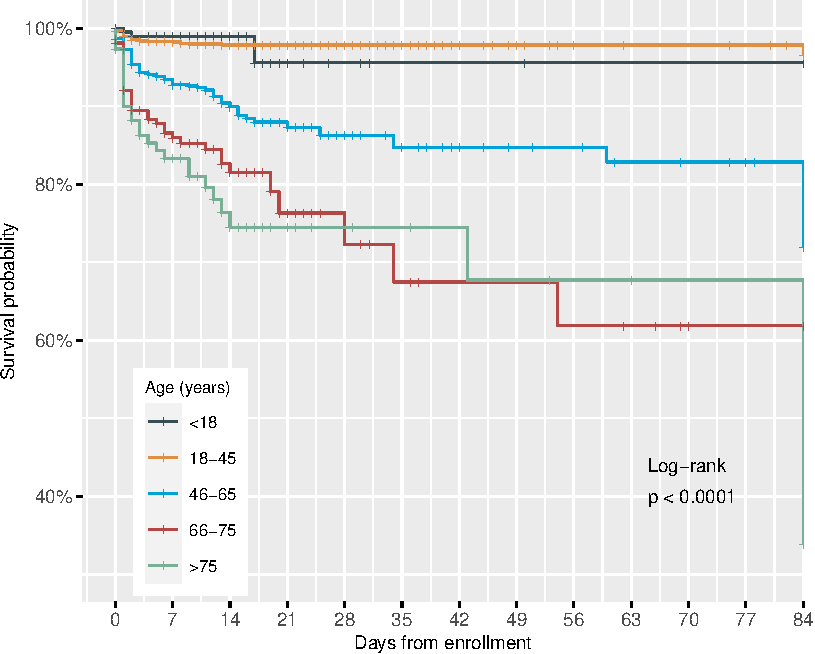
\includegraphics{results_files/figure-latex/age-1} 

}

\caption{Survival curves of patients stratified by age}\label{fig:age}
\end{figure}

\newpage

\begin{figure}[h]

{\centering 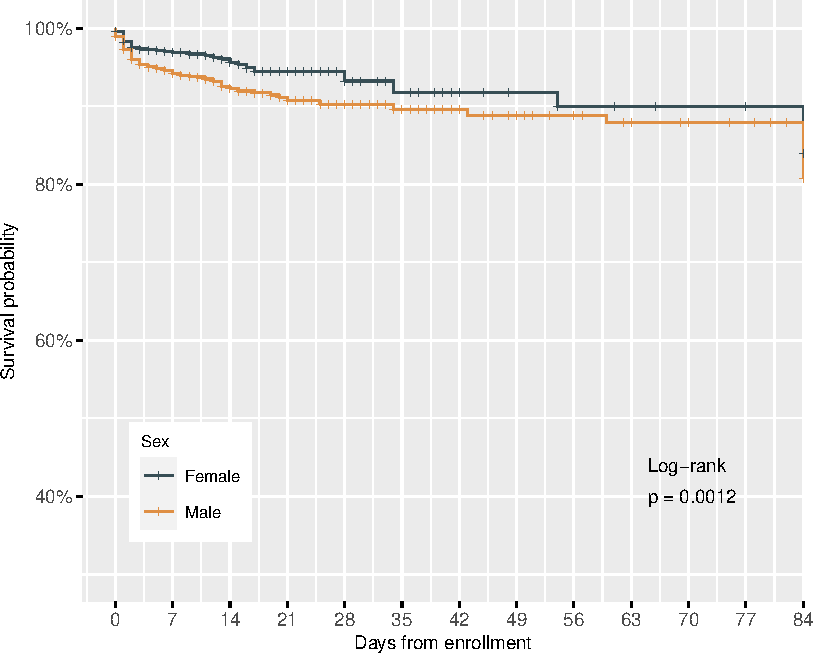
\includegraphics{results_files/figure-latex/sex-1} 

}

\caption{Survival curves of patients stratified by sex}\label{fig:sex}
\end{figure}

\newpage

\begin{figure}[h]

{\centering 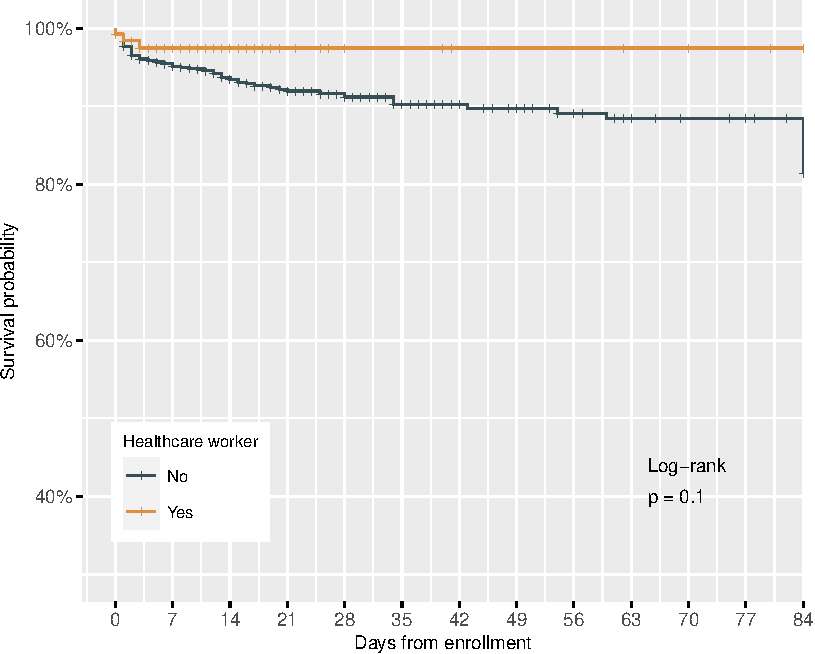
\includegraphics{results_files/figure-latex/health-worker-1} 

}

\caption{Survival curves of patients stratified by healthcare worker status}\label{fig:health-worker}
\end{figure}

\newpage

\hypertarget{comorbid-conditions}{%
\subsubsection{Comorbid conditions}\label{comorbid-conditions}}

\begin{figure}[h]

{\centering 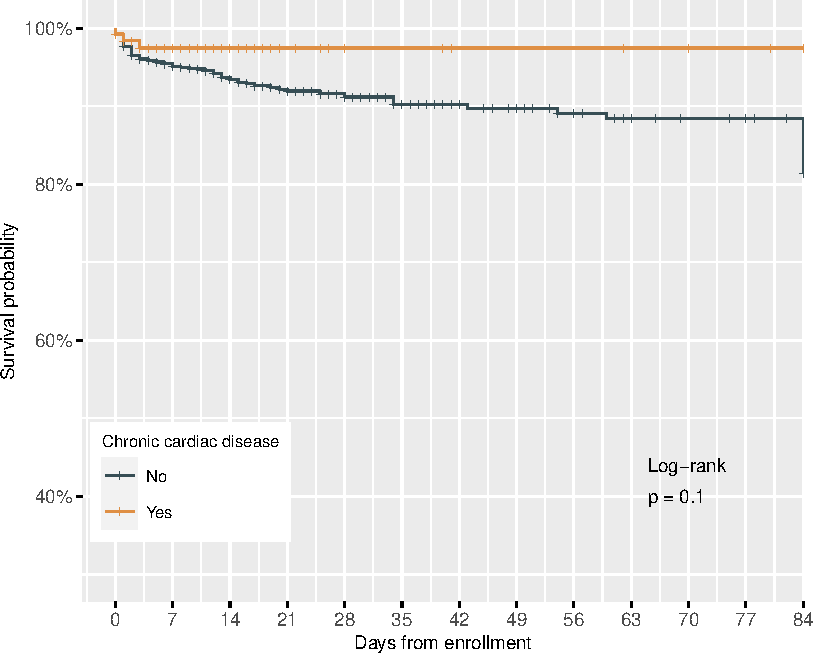
\includegraphics{results_files/figure-latex/cardiac-disease-1} 

}

\caption{Survival curves of patients stratified by chronic cardiac disease status}\label{fig:cardiac-disease}
\end{figure}

\newpage

\begin{figure}[h]

{\centering 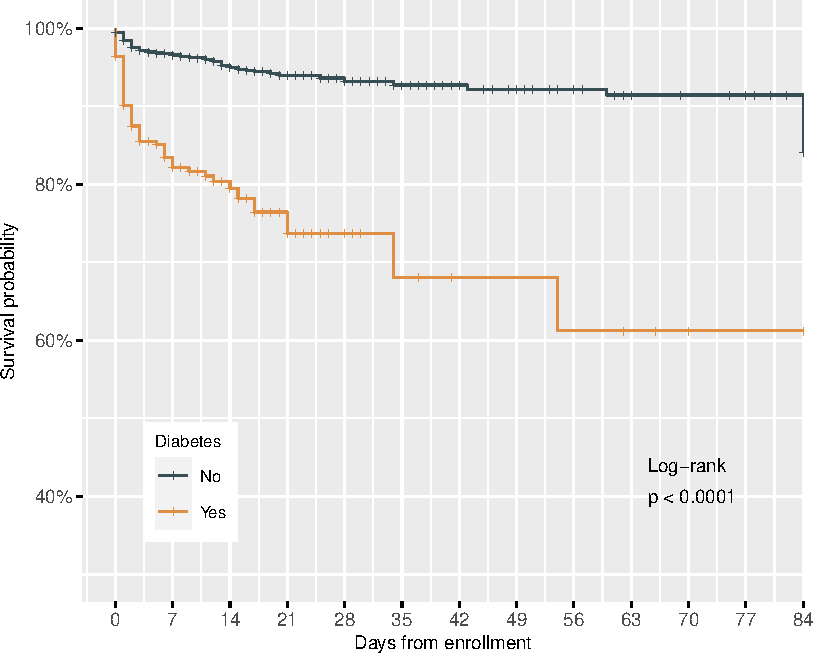
\includegraphics{results_files/figure-latex/diabetes-1} 

}

\caption{Survival curves of patients stratified by diabetes status}\label{fig:diabetes}
\end{figure}

\newpage

\begin{figure}[h]

{\centering 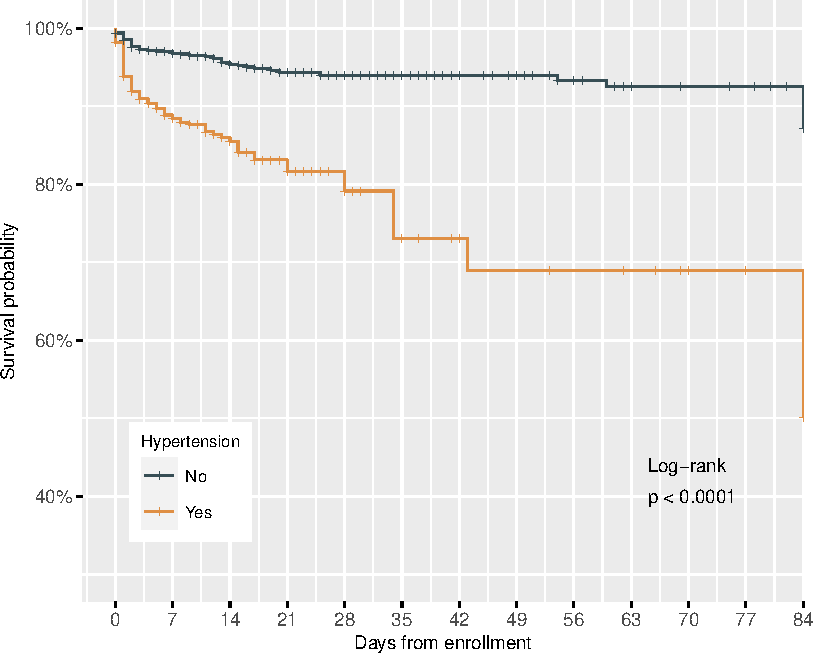
\includegraphics{results_files/figure-latex/hypertension-1} 

}

\caption{Survival curves of patients stratified by hypertension status}\label{fig:hypertension}
\end{figure}

\newpage
\begin{figure}[h]

{\centering 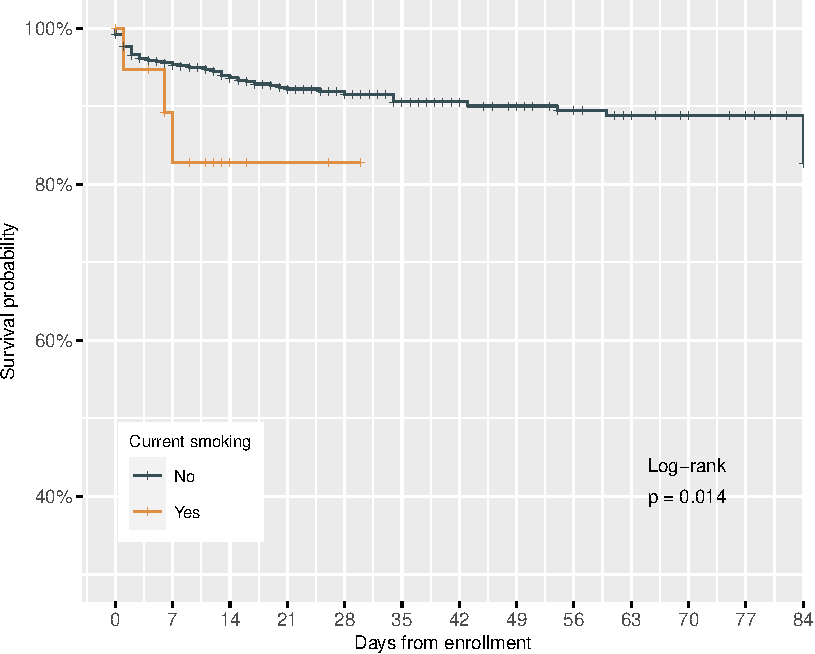
\includegraphics{results_files/figure-latex/smoking-1} 

}

\caption{Survival curves of patients stratified by current smoking status}\label{fig:smoking}
\end{figure}

\newpage
\begin{figure}[h]

{\centering 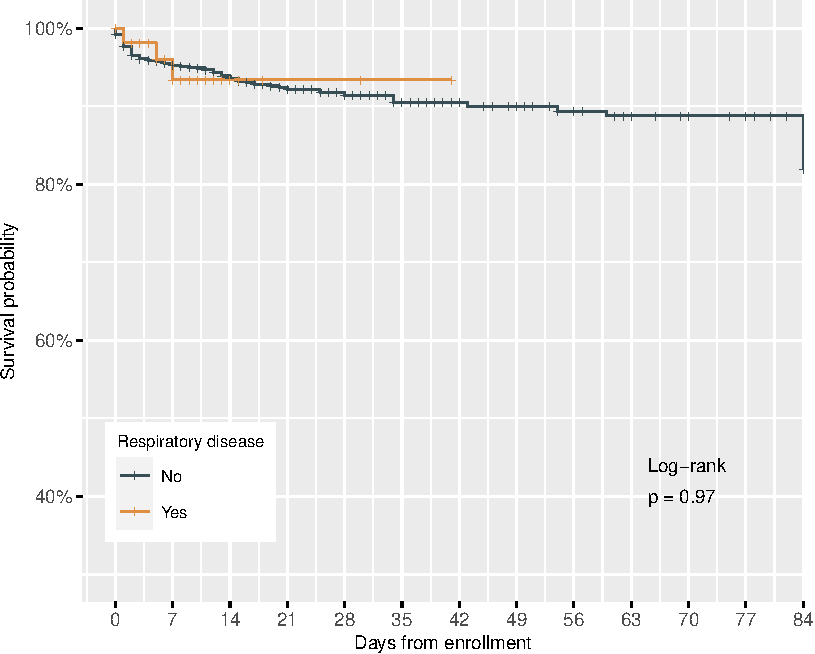
\includegraphics{results_files/figure-latex/respiratory-disease-1} 

}

\caption{Survival curves of patients stratified by respiratory disease status}\label{fig:respiratory-disease}
\end{figure}

\newpage
\begin{figure}[h]

{\centering 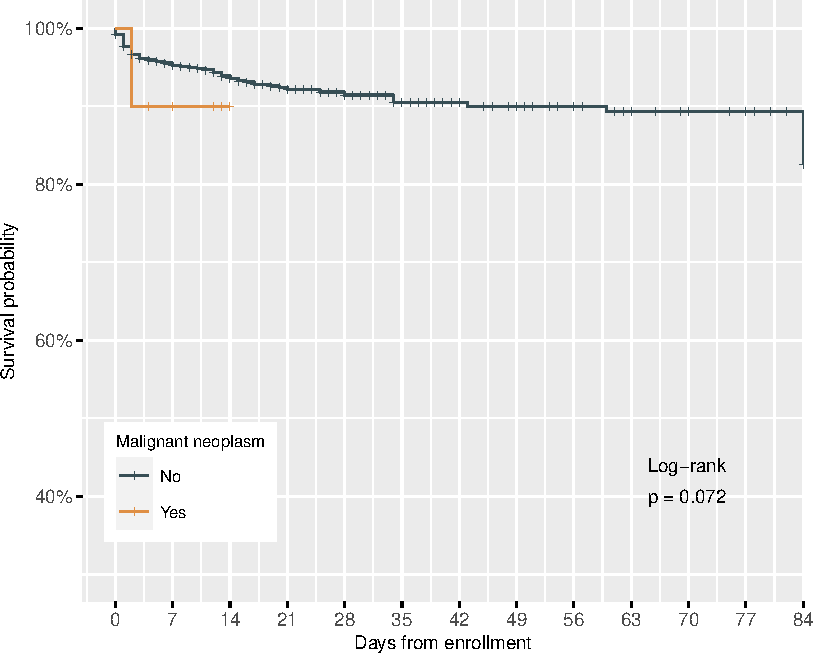
\includegraphics{results_files/figure-latex/neoplasm-1} 

}

\caption{Survival curves of patients stratified by malignant neoplasm status}\label{fig:neoplasm}
\end{figure}

\newpage
\begin{figure}[h]

{\centering 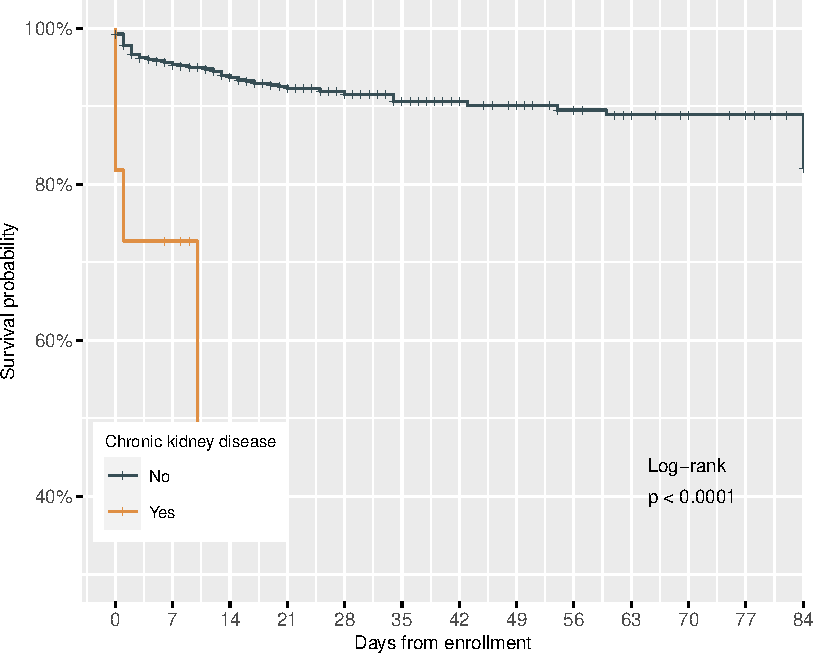
\includegraphics{results_files/figure-latex/ckd-1} 

}

\caption{Survival curves of patients stratified by chronic kidney disease status}\label{fig:ckd}
\end{figure}

\newpage
\begin{figure}[h]

{\centering 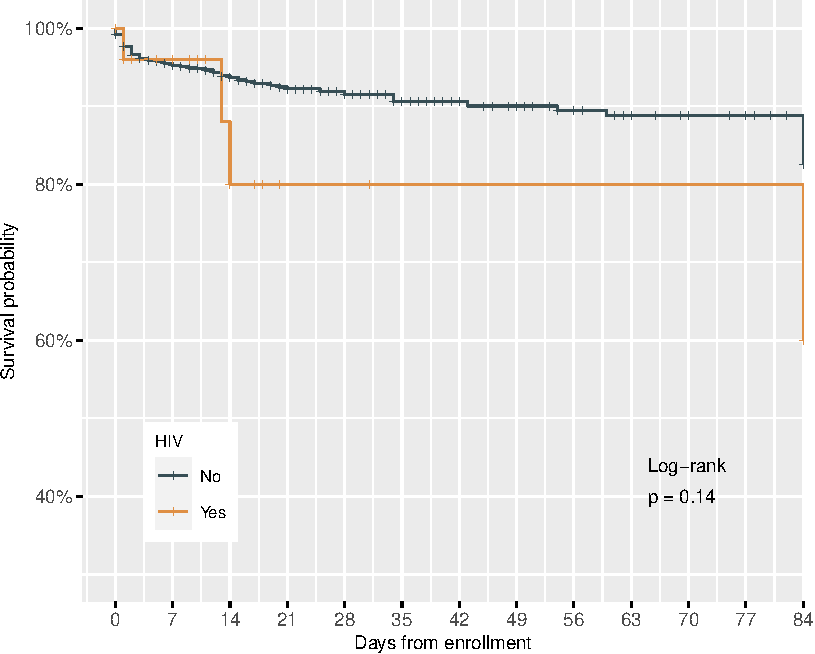
\includegraphics{results_files/figure-latex/hiv-1} 

}

\caption{Survival curves of patients stratified by HIV status}\label{fig:hiv}
\end{figure}

\newpage
\begin{figure}[h]

{\centering 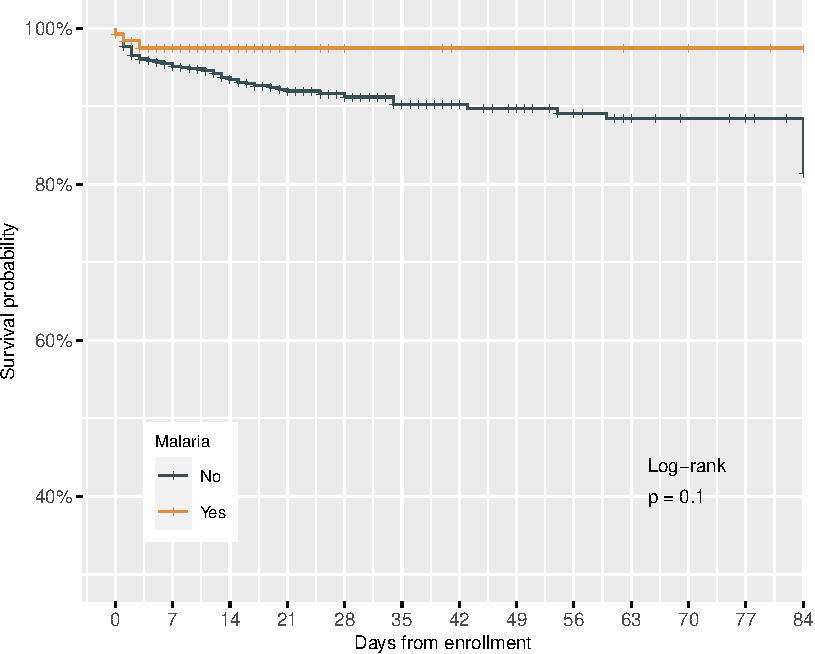
\includegraphics{results_files/figure-latex/malaria-1} 

}

\caption{Survival curves of patients stratified by malaria status}\label{fig:malaria}
\end{figure}

\newpage

\hypertarget{medications}{%
\subsubsection{Medications}\label{medications}}

\begin{figure}[h]

{\centering 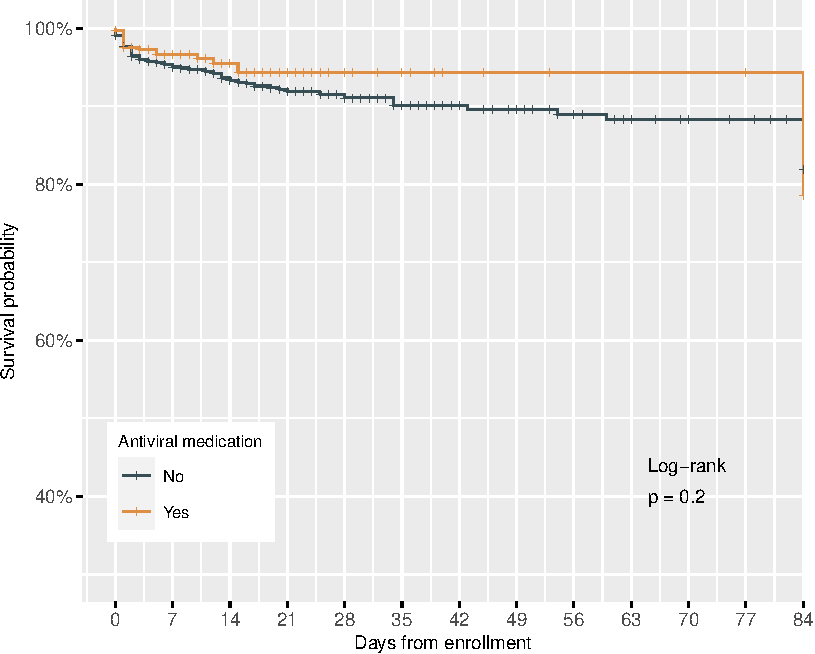
\includegraphics{results_files/figure-latex/antiviral-1} 

}

\caption{Survival curves of patients stratified by antiviral medication}\label{fig:antiviral}
\end{figure}

\newpage

\begin{figure}[h]

{\centering 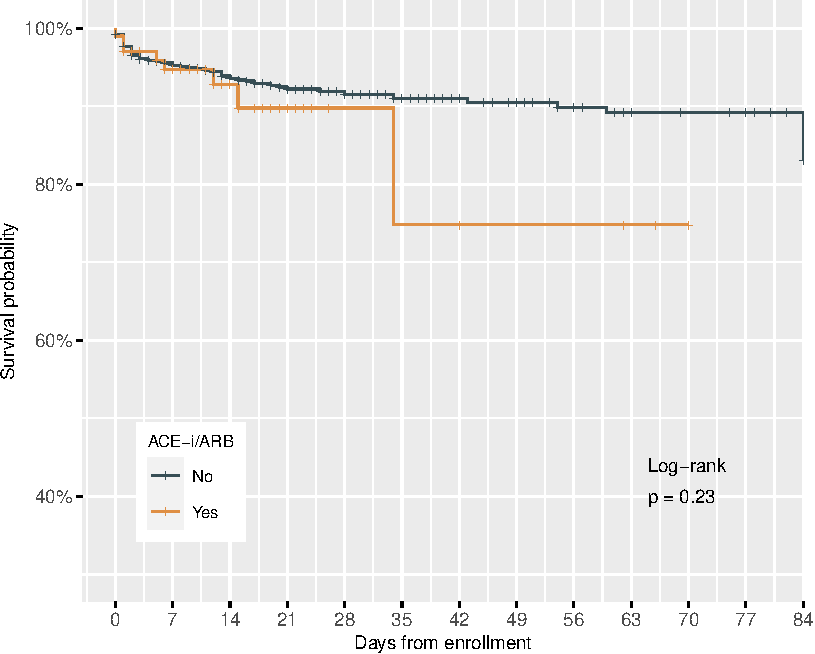
\includegraphics{results_files/figure-latex/ace-inhibitors-1} 

}

\caption{Survival curves of patients stratified by ACE-i/ARB medication}\label{fig:ace-inhibitors}
\end{figure}

\newpage
\begin{figure}[h]

{\centering 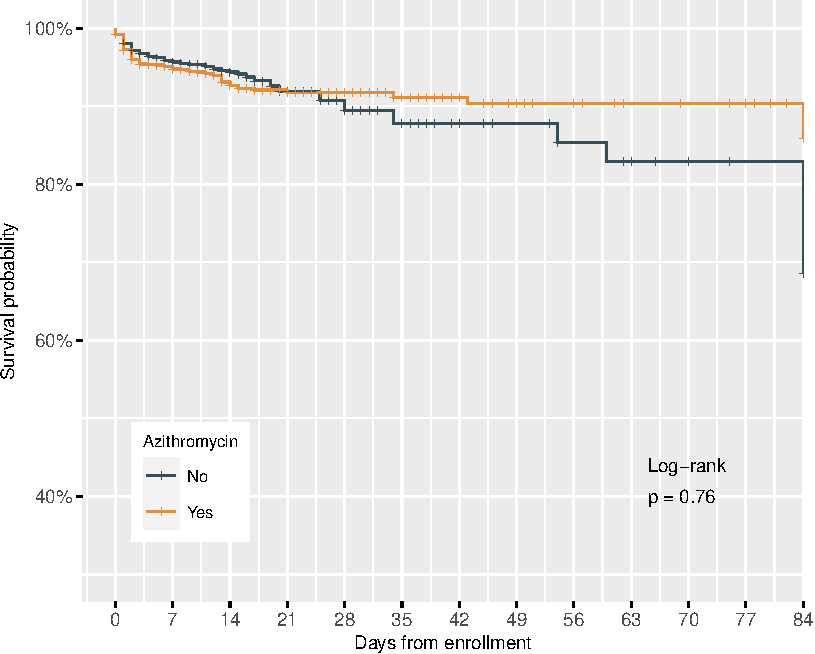
\includegraphics{results_files/figure-latex/azithromycin-1} 

}

\caption{Survival curves of patients stratified by azithromycin use}\label{fig:azithromycin}
\end{figure}

\newpage
\begin{figure}[h]

{\centering 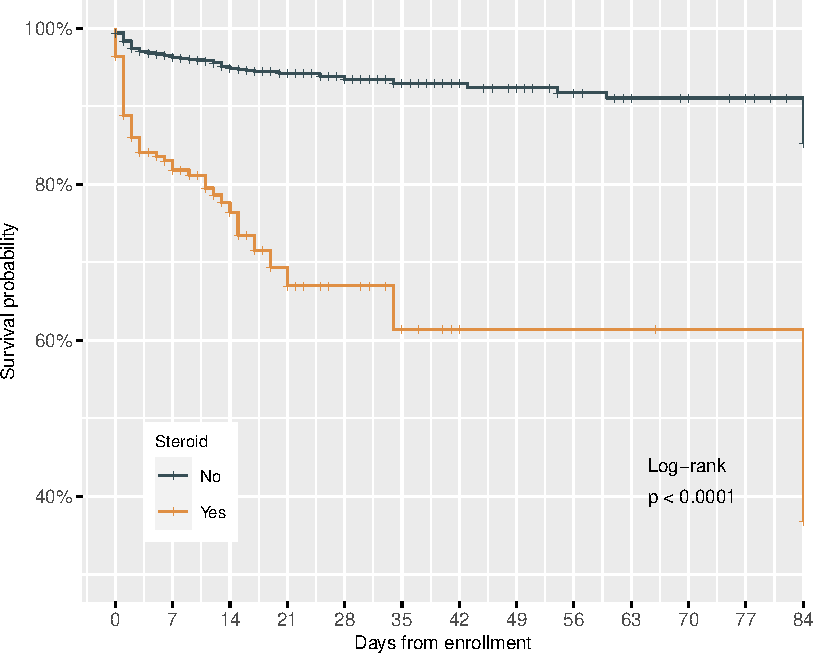
\includegraphics{results_files/figure-latex/steroid-1} 

}

\caption{Survival curves of patients stratified by steroid use}\label{fig:steroid}
\end{figure}

\newpage
\begin{figure}[h]

{\centering 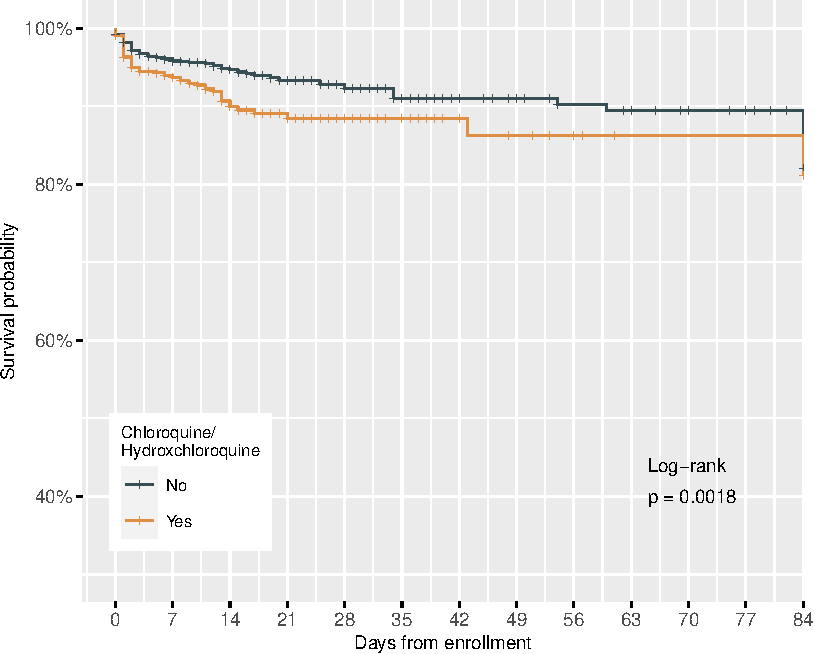
\includegraphics{results_files/figure-latex/chloroquine-1} 

}

\caption{Survival curves of patients stratified by chloroquine/hydroxychloroquine use}\label{fig:chloroquine}
\end{figure}

\newpage
\begin{figure}[h]

{\centering 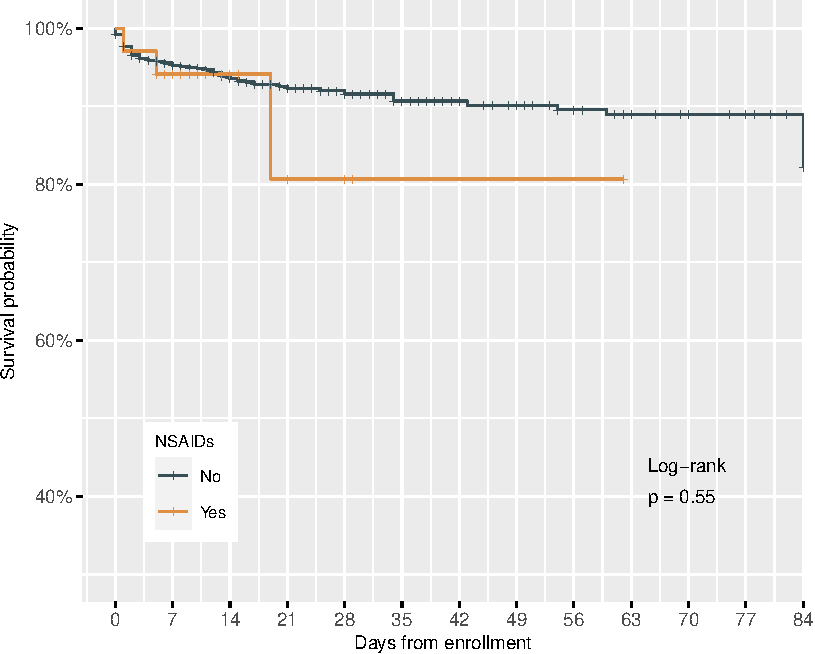
\includegraphics{results_files/figure-latex/nsaids-1} 

}

\caption{Survival curves of patients stratified by NSAIDs use}\label{fig:nsaids}
\end{figure}

\newpage
\begin{figure}[h]

{\centering 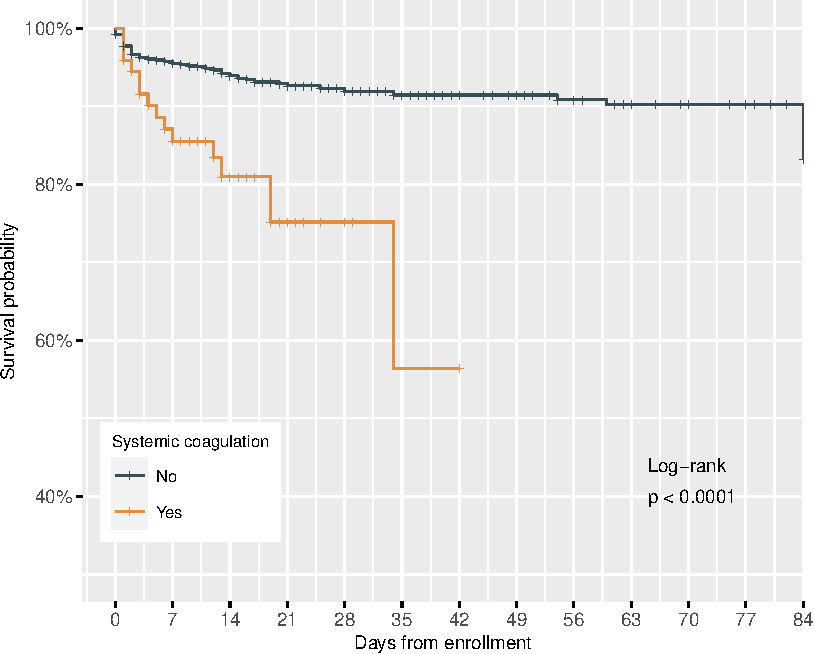
\includegraphics{results_files/figure-latex/coagulation-1} 

}

\caption{Survival curves of patients stratified by systemic coagulation status}\label{fig:coagulation}
\end{figure}

\newpage

\hypertarget{logistic-regression-model}{%
\subsection{Logistic regression model}\label{logistic-regression-model}}

We fitted a mixed effects logistic regression model using maximum
likelihood and the bound optimization by quadratic approximation
algorithm to predict mortality with severity, age group, male gender,
health worker status, chronic cardiac disease, diabetes, respiratory
disease ((defined as presence of any of chronic pulmonary disease,
active or previous tuberculosis, and asthma), chronic kidney disease,
malaria, azithromycin and chloroquine entered into the model as fixed
effects. The model included site and facility type as random effects.
The most parsimonious model arrived at through backward stepwise
regression is shown in Table \ref{tab:logistic-regression} below.

The model's total explanatory power is substantial (conditional
\emph{R}² = 0.55) and the part related to the fixed effects alone
(marginal \emph{R}²) is of 0.25. The intra-class correlation coefficient
(ICC) = 0.40. The conditional \emph{R}² is the proportion of overall
variance explained by the model when the site and facility type random
effects are taken into account. The marginal \emph{R}² is the proportion
of the overall variance explained by the fixed effects only. The ICC is
a measure of the correlation between patients within clusters. It ranges
from 0 to 1. Confidence Intervals (CIs) at the 95\% level and p-values
were computed using the Wald approximation.

 
  \providecommand{\huxb}[2]{\arrayrulecolor[RGB]{#1}\global\arrayrulewidth=#2pt}
  \providecommand{\huxvb}[2]{\color[RGB]{#1}\vrule width #2pt}
  \providecommand{\huxtpad}[1]{\rule{0pt}{#1}}
  \providecommand{\huxbpad}[1]{\rule[-#1]{0pt}{#1}}

\begin{table}[h!]
\begin{centerbox}
\begin{threeparttable}
\captionsetup{justification=centering,singlelinecheck=off}
\caption{Mixed effects logistic regression model of predictors of mortality}
 \label{tab:logistic-regression}
\setlength{\tabcolsep}{0pt}
\begin{tabularx}{0.96\textwidth}{p{0.48\textwidth} p{0.192\textwidth} p{0.192\textwidth} p{0.096\textwidth}}


\hhline{>{\huxb{0, 0, 0}{0.4}}->{\huxb{0, 0, 0}{0.4}}->{\huxb{0, 0, 0}{0.4}}->{\huxb{0, 0, 0}{0.4}}-}
\arrayrulecolor{black}

\multicolumn{1}{!{\huxvb{0, 0, 0}{0}}p{0.48\textwidth}!{\huxvb{0, 0, 0}{0}}}{\cellcolor[RGB]{255, 255, 255}\hspace{6pt}\parbox[b]{0.48\textwidth-6pt-6pt}{\huxtpad{1pt + 1em}\raggedright {\fontsize{8pt}{9.6pt}\selectfont \textbf{Predictors}
}\huxbpad{1pt}}} &
\multicolumn{1}{p{0.192\textwidth}!{\huxvb{0, 0, 0}{0}}}{\cellcolor[RGB]{255, 255, 255}\hspace{6pt}\parbox[b]{0.192\textwidth-6pt-6pt}{\huxtpad{1pt + 1em}\raggedleft {\fontsize{8pt}{9.6pt}\selectfont \textbf{OR}
\hphantom{0}\hphantom{0}\hphantom{0}}\huxbpad{1pt}}} &
\multicolumn{1}{p{0.192\textwidth}!{\huxvb{0, 0, 0}{0}}}{\cellcolor[RGB]{255, 255, 255}\hspace{6pt}\parbox[b]{0.192\textwidth-6pt-6pt}{\huxtpad{1pt + 1em}\centering {\fontsize{8pt}{9.6pt}\selectfont \textbf{95\% CI}
}\huxbpad{1pt}}} &
\multicolumn{1}{p{0.096\textwidth}!{\huxvb{0, 0, 0}{0}}}{\cellcolor[RGB]{255, 255, 255}\hspace{6pt}\parbox[b]{0.096\textwidth-6pt-6pt}{\huxtpad{1pt + 1em}\raggedleft {\fontsize{8pt}{9.6pt}\selectfont \emph{p} value
}\huxbpad{1pt}}} \tabularnewline[-0.5pt]


\hhline{>{\huxb{0, 0, 0}{0.4}}->{\huxb{0, 0, 0}{0.4}}->{\huxb{0, 0, 0}{0.4}}->{\huxb{0, 0, 0}{0.4}}-}
\arrayrulecolor{black}

\multicolumn{1}{!{\huxvb{0, 0, 0}{0}}p{0.48\textwidth}!{\huxvb{0, 0, 0}{0}}}{\cellcolor[RGB]{240, 240, 240}\hspace{6pt}\parbox[b]{0.48\textwidth-6pt-6pt}{\huxtpad{1pt + 1em}\raggedright {\fontsize{8pt}{9.6pt}\selectfont Severity score}\huxbpad{1pt}}} &
\multicolumn{1}{p{0.192\textwidth}!{\huxvb{0, 0, 0}{0}}}{\cellcolor[RGB]{240, 240, 240}\hspace{6pt}\parbox[b]{0.192\textwidth-6pt-6pt}{\huxtpad{1pt + 1em}\raggedleft {\fontsize{8pt}{9.6pt}\selectfont 3.50}\huxbpad{1pt}}} &
\multicolumn{1}{p{0.192\textwidth}!{\huxvb{0, 0, 0}{0}}}{\cellcolor[RGB]{240, 240, 240}\hspace{6pt}\parbox[b]{0.192\textwidth-6pt-6pt}{\huxtpad{1pt + 1em}\centering {\fontsize{8pt}{9.6pt}\selectfont 2.73, 4.49}\huxbpad{1pt}}} &
\multicolumn{1}{p{0.096\textwidth}!{\huxvb{0, 0, 0}{0}}}{\cellcolor[RGB]{240, 240, 240}\hspace{6pt}\parbox[b]{0.096\textwidth-6pt-6pt}{\huxtpad{1pt + 1em}\raggedleft {\fontsize{8pt}{9.6pt}\selectfont $<$0.001}\huxbpad{1pt}}} \tabularnewline[-0.5pt]


\hhline{}
\arrayrulecolor{black}

\multicolumn{1}{!{\huxvb{0, 0, 0}{0}}p{0.48\textwidth}!{\huxvb{0, 0, 0}{0}}}{\cellcolor[RGB]{255, 255, 255}\hspace{6pt}\parbox[b]{0.48\textwidth-6pt-6pt}{\huxtpad{1pt + 1em}\raggedright {\fontsize{8pt}{9.6pt}\selectfont Age group}\huxbpad{1pt}}} &
\multicolumn{1}{p{0.192\textwidth}!{\huxvb{0, 0, 0}{0}}}{\cellcolor[RGB]{255, 255, 255}\hspace{6pt}\parbox[b]{0.192\textwidth-6pt-6pt}{\huxtpad{1pt + 1em}\raggedleft {\fontsize{8pt}{9.6pt}\selectfont \hphantom{0}\hphantom{0}\hphantom{0}}\huxbpad{1pt}}} &
\multicolumn{1}{p{0.192\textwidth}!{\huxvb{0, 0, 0}{0}}}{\cellcolor[RGB]{255, 255, 255}\hspace{6pt}\parbox[b]{0.192\textwidth-6pt-6pt}{\huxtpad{1pt + 1em}\centering {\fontsize{8pt}{9.6pt}\selectfont }\huxbpad{1pt}}} &
\multicolumn{1}{p{0.096\textwidth}!{\huxvb{0, 0, 0}{0}}}{\cellcolor[RGB]{255, 255, 255}\hspace{6pt}\parbox[b]{0.096\textwidth-6pt-6pt}{\huxtpad{1pt + 1em}\raggedleft {\fontsize{8pt}{9.6pt}\selectfont }\huxbpad{1pt}}} \tabularnewline[-0.5pt]


\hhline{}
\arrayrulecolor{black}

\multicolumn{1}{!{\huxvb{0, 0, 0}{0}}p{0.48\textwidth}!{\huxvb{0, 0, 0}{0}}}{\cellcolor[RGB]{240, 240, 240}\hspace{15pt}\parbox[b]{0.48\textwidth-15pt-6pt}{\huxtpad{1pt + 1em}\raggedright {\fontsize{8pt}{9.6pt}\selectfont $<$18}\huxbpad{1pt}}} &
\multicolumn{1}{p{0.192\textwidth}!{\huxvb{0, 0, 0}{0}}}{\cellcolor[RGB]{240, 240, 240}\hspace{6pt}\parbox[b]{0.192\textwidth-6pt-6pt}{\huxtpad{1pt + 1em}\raggedleft {\fontsize{8pt}{9.6pt}\selectfont ...\hphantom{0}\hphantom{0}}\huxbpad{1pt}}} &
\multicolumn{1}{p{0.192\textwidth}!{\huxvb{0, 0, 0}{0}}}{\cellcolor[RGB]{240, 240, 240}\hspace{6pt}\parbox[b]{0.192\textwidth-6pt-6pt}{\huxtpad{1pt + 1em}\centering {\fontsize{8pt}{9.6pt}\selectfont ...}\huxbpad{1pt}}} &
\multicolumn{1}{p{0.096\textwidth}!{\huxvb{0, 0, 0}{0}}}{\cellcolor[RGB]{240, 240, 240}\hspace{6pt}\parbox[b]{0.096\textwidth-6pt-6pt}{\huxtpad{1pt + 1em}\raggedleft {\fontsize{8pt}{9.6pt}\selectfont }\huxbpad{1pt}}} \tabularnewline[-0.5pt]


\hhline{}
\arrayrulecolor{black}

\multicolumn{1}{!{\huxvb{0, 0, 0}{0}}p{0.48\textwidth}!{\huxvb{0, 0, 0}{0}}}{\cellcolor[RGB]{255, 255, 255}\hspace{15pt}\parbox[b]{0.48\textwidth-15pt-6pt}{\huxtpad{1pt + 1em}\raggedright {\fontsize{8pt}{9.6pt}\selectfont 18$-$45}\huxbpad{1pt}}} &
\multicolumn{1}{p{0.192\textwidth}!{\huxvb{0, 0, 0}{0}}}{\cellcolor[RGB]{255, 255, 255}\hspace{6pt}\parbox[b]{0.192\textwidth-6pt-6pt}{\huxtpad{1pt + 1em}\raggedleft {\fontsize{8pt}{9.6pt}\selectfont 1.81}\huxbpad{1pt}}} &
\multicolumn{1}{p{0.192\textwidth}!{\huxvb{0, 0, 0}{0}}}{\cellcolor[RGB]{255, 255, 255}\hspace{6pt}\parbox[b]{0.192\textwidth-6pt-6pt}{\huxtpad{1pt + 1em}\centering {\fontsize{8pt}{9.6pt}\selectfont 0.58, 5.61}\huxbpad{1pt}}} &
\multicolumn{1}{p{0.096\textwidth}!{\huxvb{0, 0, 0}{0}}}{\cellcolor[RGB]{255, 255, 255}\hspace{6pt}\parbox[b]{0.096\textwidth-6pt-6pt}{\huxtpad{1pt + 1em}\raggedleft {\fontsize{8pt}{9.6pt}\selectfont 0.307}\huxbpad{1pt}}} \tabularnewline[-0.5pt]


\hhline{}
\arrayrulecolor{black}

\multicolumn{1}{!{\huxvb{0, 0, 0}{0}}p{0.48\textwidth}!{\huxvb{0, 0, 0}{0}}}{\cellcolor[RGB]{240, 240, 240}\hspace{15pt}\parbox[b]{0.48\textwidth-15pt-6pt}{\huxtpad{1pt + 1em}\raggedright {\fontsize{8pt}{9.6pt}\selectfont 46$-$65}\huxbpad{1pt}}} &
\multicolumn{1}{p{0.192\textwidth}!{\huxvb{0, 0, 0}{0}}}{\cellcolor[RGB]{240, 240, 240}\hspace{6pt}\parbox[b]{0.192\textwidth-6pt-6pt}{\huxtpad{1pt + 1em}\raggedleft {\fontsize{8pt}{9.6pt}\selectfont 3.93}\huxbpad{1pt}}} &
\multicolumn{1}{p{0.192\textwidth}!{\huxvb{0, 0, 0}{0}}}{\cellcolor[RGB]{240, 240, 240}\hspace{6pt}\parbox[b]{0.192\textwidth-6pt-6pt}{\huxtpad{1pt + 1em}\centering {\fontsize{8pt}{9.6pt}\selectfont 1.29, 12.02}\huxbpad{1pt}}} &
\multicolumn{1}{p{0.096\textwidth}!{\huxvb{0, 0, 0}{0}}}{\cellcolor[RGB]{240, 240, 240}\hspace{6pt}\parbox[b]{0.096\textwidth-6pt-6pt}{\huxtpad{1pt + 1em}\raggedleft {\fontsize{8pt}{9.6pt}\selectfont 0.016}\huxbpad{1pt}}} \tabularnewline[-0.5pt]


\hhline{}
\arrayrulecolor{black}

\multicolumn{1}{!{\huxvb{0, 0, 0}{0}}p{0.48\textwidth}!{\huxvb{0, 0, 0}{0}}}{\cellcolor[RGB]{255, 255, 255}\hspace{15pt}\parbox[b]{0.48\textwidth-15pt-6pt}{\huxtpad{1pt + 1em}\raggedright {\fontsize{8pt}{9.6pt}\selectfont 66$-$75}\huxbpad{1pt}}} &
\multicolumn{1}{p{0.192\textwidth}!{\huxvb{0, 0, 0}{0}}}{\cellcolor[RGB]{255, 255, 255}\hspace{6pt}\parbox[b]{0.192\textwidth-6pt-6pt}{\huxtpad{1pt + 1em}\raggedleft {\fontsize{8pt}{9.6pt}\selectfont 5.37}\huxbpad{1pt}}} &
\multicolumn{1}{p{0.192\textwidth}!{\huxvb{0, 0, 0}{0}}}{\cellcolor[RGB]{255, 255, 255}\hspace{6pt}\parbox[b]{0.192\textwidth-6pt-6pt}{\huxtpad{1pt + 1em}\centering {\fontsize{8pt}{9.6pt}\selectfont 1.68, 17.14}\huxbpad{1pt}}} &
\multicolumn{1}{p{0.096\textwidth}!{\huxvb{0, 0, 0}{0}}}{\cellcolor[RGB]{255, 255, 255}\hspace{6pt}\parbox[b]{0.096\textwidth-6pt-6pt}{\huxtpad{1pt + 1em}\raggedleft {\fontsize{8pt}{9.6pt}\selectfont 0.005}\huxbpad{1pt}}} \tabularnewline[-0.5pt]


\hhline{}
\arrayrulecolor{black}

\multicolumn{1}{!{\huxvb{0, 0, 0}{0}}p{0.48\textwidth}!{\huxvb{0, 0, 0}{0}}}{\cellcolor[RGB]{240, 240, 240}\hspace{15pt}\parbox[b]{0.48\textwidth-15pt-6pt}{\huxtpad{1pt + 1em}\raggedright {\fontsize{8pt}{9.6pt}\selectfont $>$75}\huxbpad{1pt}}} &
\multicolumn{1}{p{0.192\textwidth}!{\huxvb{0, 0, 0}{0}}}{\cellcolor[RGB]{240, 240, 240}\hspace{6pt}\parbox[b]{0.192\textwidth-6pt-6pt}{\huxtpad{1pt + 1em}\raggedleft {\fontsize{8pt}{9.6pt}\selectfont 6.81}\huxbpad{1pt}}} &
\multicolumn{1}{p{0.192\textwidth}!{\huxvb{0, 0, 0}{0}}}{\cellcolor[RGB]{240, 240, 240}\hspace{6pt}\parbox[b]{0.192\textwidth-6pt-6pt}{\huxtpad{1pt + 1em}\centering {\fontsize{8pt}{9.6pt}\selectfont 2.04, 22.81}\huxbpad{1pt}}} &
\multicolumn{1}{p{0.096\textwidth}!{\huxvb{0, 0, 0}{0}}}{\cellcolor[RGB]{240, 240, 240}\hspace{6pt}\parbox[b]{0.096\textwidth-6pt-6pt}{\huxtpad{1pt + 1em}\raggedleft {\fontsize{8pt}{9.6pt}\selectfont 0.002}\huxbpad{1pt}}} \tabularnewline[-0.5pt]


\hhline{}
\arrayrulecolor{black}

\multicolumn{1}{!{\huxvb{0, 0, 0}{0}}p{0.48\textwidth}!{\huxvb{0, 0, 0}{0}}}{\cellcolor[RGB]{255, 255, 255}\hspace{6pt}\parbox[b]{0.48\textwidth-6pt-6pt}{\huxtpad{1pt + 1em}\raggedright {\fontsize{8pt}{9.6pt}\selectfont Male}\huxbpad{1pt}}} &
\multicolumn{1}{p{0.192\textwidth}!{\huxvb{0, 0, 0}{0}}}{\cellcolor[RGB]{255, 255, 255}\hspace{6pt}\parbox[b]{0.192\textwidth-6pt-6pt}{\huxtpad{1pt + 1em}\raggedleft {\fontsize{8pt}{9.6pt}\selectfont 1.78}\huxbpad{1pt}}} &
\multicolumn{1}{p{0.192\textwidth}!{\huxvb{0, 0, 0}{0}}}{\cellcolor[RGB]{255, 255, 255}\hspace{6pt}\parbox[b]{0.192\textwidth-6pt-6pt}{\huxtpad{1pt + 1em}\centering {\fontsize{8pt}{9.6pt}\selectfont 1.23, 2.56}\huxbpad{1pt}}} &
\multicolumn{1}{p{0.096\textwidth}!{\huxvb{0, 0, 0}{0}}}{\cellcolor[RGB]{255, 255, 255}\hspace{6pt}\parbox[b]{0.096\textwidth-6pt-6pt}{\huxtpad{1pt + 1em}\raggedleft {\fontsize{8pt}{9.6pt}\selectfont 0.002}\huxbpad{1pt}}} \tabularnewline[-0.5pt]


\hhline{}
\arrayrulecolor{black}

\multicolumn{1}{!{\huxvb{0, 0, 0}{0}}p{0.48\textwidth}!{\huxvb{0, 0, 0}{0}}}{\cellcolor[RGB]{240, 240, 240}\hspace{6pt}\parbox[b]{0.48\textwidth-6pt-6pt}{\huxtpad{1pt + 1em}\raggedright {\fontsize{8pt}{9.6pt}\selectfont Health care worker}\huxbpad{1pt}}} &
\multicolumn{1}{p{0.192\textwidth}!{\huxvb{0, 0, 0}{0}}}{\cellcolor[RGB]{240, 240, 240}\hspace{6pt}\parbox[b]{0.192\textwidth-6pt-6pt}{\huxtpad{1pt + 1em}\raggedleft {\fontsize{8pt}{9.6pt}\selectfont 0.22}\huxbpad{1pt}}} &
\multicolumn{1}{p{0.192\textwidth}!{\huxvb{0, 0, 0}{0}}}{\cellcolor[RGB]{240, 240, 240}\hspace{6pt}\parbox[b]{0.192\textwidth-6pt-6pt}{\huxtpad{1pt + 1em}\centering {\fontsize{8pt}{9.6pt}\selectfont 0.06, 0.79}\huxbpad{1pt}}} &
\multicolumn{1}{p{0.096\textwidth}!{\huxvb{0, 0, 0}{0}}}{\cellcolor[RGB]{240, 240, 240}\hspace{6pt}\parbox[b]{0.096\textwidth-6pt-6pt}{\huxtpad{1pt + 1em}\raggedleft {\fontsize{8pt}{9.6pt}\selectfont 0.020}\huxbpad{1pt}}} \tabularnewline[-0.5pt]


\hhline{}
\arrayrulecolor{black}

\multicolumn{1}{!{\huxvb{0, 0, 0}{0}}p{0.48\textwidth}!{\huxvb{0, 0, 0}{0}}}{\cellcolor[RGB]{255, 255, 255}\hspace{6pt}\parbox[b]{0.48\textwidth-6pt-6pt}{\huxtpad{1pt + 1em}\raggedright {\fontsize{8pt}{9.6pt}\selectfont Chronic cardiac disease (not hypertension)}\huxbpad{1pt}}} &
\multicolumn{1}{p{0.192\textwidth}!{\huxvb{0, 0, 0}{0}}}{\cellcolor[RGB]{255, 255, 255}\hspace{6pt}\parbox[b]{0.192\textwidth-6pt-6pt}{\huxtpad{1pt + 1em}\raggedleft {\fontsize{8pt}{9.6pt}\selectfont 3.07}\huxbpad{1pt}}} &
\multicolumn{1}{p{0.192\textwidth}!{\huxvb{0, 0, 0}{0}}}{\cellcolor[RGB]{255, 255, 255}\hspace{6pt}\parbox[b]{0.192\textwidth-6pt-6pt}{\huxtpad{1pt + 1em}\centering {\fontsize{8pt}{9.6pt}\selectfont 1.20, 7.86}\huxbpad{1pt}}} &
\multicolumn{1}{p{0.096\textwidth}!{\huxvb{0, 0, 0}{0}}}{\cellcolor[RGB]{255, 255, 255}\hspace{6pt}\parbox[b]{0.096\textwidth-6pt-6pt}{\huxtpad{1pt + 1em}\raggedleft {\fontsize{8pt}{9.6pt}\selectfont 0.019}\huxbpad{1pt}}} \tabularnewline[-0.5pt]


\hhline{}
\arrayrulecolor{black}

\multicolumn{1}{!{\huxvb{0, 0, 0}{0}}p{0.48\textwidth}!{\huxvb{0, 0, 0}{0}}}{\cellcolor[RGB]{240, 240, 240}\hspace{6pt}\parbox[b]{0.48\textwidth-6pt-6pt}{\huxtpad{1pt + 1em}\raggedright {\fontsize{8pt}{9.6pt}\selectfont Diabetes}\huxbpad{1pt}}} &
\multicolumn{1}{p{0.192\textwidth}!{\huxvb{0, 0, 0}{0}}}{\cellcolor[RGB]{240, 240, 240}\hspace{6pt}\parbox[b]{0.192\textwidth-6pt-6pt}{\huxtpad{1pt + 1em}\raggedleft {\fontsize{8pt}{9.6pt}\selectfont 2.16}\huxbpad{1pt}}} &
\multicolumn{1}{p{0.192\textwidth}!{\huxvb{0, 0, 0}{0}}}{\cellcolor[RGB]{240, 240, 240}\hspace{6pt}\parbox[b]{0.192\textwidth-6pt-6pt}{\huxtpad{1pt + 1em}\centering {\fontsize{8pt}{9.6pt}\selectfont 1.41, 3.31}\huxbpad{1pt}}} &
\multicolumn{1}{p{0.096\textwidth}!{\huxvb{0, 0, 0}{0}}}{\cellcolor[RGB]{240, 240, 240}\hspace{6pt}\parbox[b]{0.096\textwidth-6pt-6pt}{\huxtpad{1pt + 1em}\raggedleft {\fontsize{8pt}{9.6pt}\selectfont $<$0.001}\huxbpad{1pt}}} \tabularnewline[-0.5pt]


\hhline{}
\arrayrulecolor{black}

\multicolumn{1}{!{\huxvb{0, 0, 0}{0}}p{0.48\textwidth}!{\huxvb{0, 0, 0}{0}}}{\cellcolor[RGB]{255, 255, 255}\hspace{6pt}\parbox[b]{0.48\textwidth-6pt-6pt}{\huxtpad{1pt + 1em}\raggedright {\fontsize{8pt}{9.6pt}\selectfont Respiratory disease}\huxbpad{1pt}}} &
\multicolumn{1}{p{0.192\textwidth}!{\huxvb{0, 0, 0}{0}}}{\cellcolor[RGB]{255, 255, 255}\hspace{6pt}\parbox[b]{0.192\textwidth-6pt-6pt}{\huxtpad{1pt + 1em}\raggedleft {\fontsize{8pt}{9.6pt}\selectfont 0.34}\huxbpad{1pt}}} &
\multicolumn{1}{p{0.192\textwidth}!{\huxvb{0, 0, 0}{0}}}{\cellcolor[RGB]{255, 255, 255}\hspace{6pt}\parbox[b]{0.192\textwidth-6pt-6pt}{\huxtpad{1pt + 1em}\centering {\fontsize{8pt}{9.6pt}\selectfont 0.09, 1.20}\huxbpad{1pt}}} &
\multicolumn{1}{p{0.096\textwidth}!{\huxvb{0, 0, 0}{0}}}{\cellcolor[RGB]{255, 255, 255}\hspace{6pt}\parbox[b]{0.096\textwidth-6pt-6pt}{\huxtpad{1pt + 1em}\raggedleft {\fontsize{8pt}{9.6pt}\selectfont 0.094}\huxbpad{1pt}}} \tabularnewline[-0.5pt]


\hhline{}
\arrayrulecolor{black}

\multicolumn{1}{!{\huxvb{0, 0, 0}{0}}p{0.48\textwidth}!{\huxvb{0, 0, 0}{0}}}{\cellcolor[RGB]{240, 240, 240}\hspace{6pt}\parbox[b]{0.48\textwidth-6pt-6pt}{\huxtpad{1pt + 1em}\raggedright {\fontsize{8pt}{9.6pt}\selectfont Chronic kidney disease}\huxbpad{1pt}}} &
\multicolumn{1}{p{0.192\textwidth}!{\huxvb{0, 0, 0}{0}}}{\cellcolor[RGB]{240, 240, 240}\hspace{6pt}\parbox[b]{0.192\textwidth-6pt-6pt}{\huxtpad{1pt + 1em}\raggedleft {\fontsize{8pt}{9.6pt}\selectfont 11.01}\huxbpad{1pt}}} &
\multicolumn{1}{p{0.192\textwidth}!{\huxvb{0, 0, 0}{0}}}{\cellcolor[RGB]{240, 240, 240}\hspace{6pt}\parbox[b]{0.192\textwidth-6pt-6pt}{\huxtpad{1pt + 1em}\centering {\fontsize{8pt}{9.6pt}\selectfont 2.74, 44.25}\huxbpad{1pt}}} &
\multicolumn{1}{p{0.096\textwidth}!{\huxvb{0, 0, 0}{0}}}{\cellcolor[RGB]{240, 240, 240}\hspace{6pt}\parbox[b]{0.096\textwidth-6pt-6pt}{\huxtpad{1pt + 1em}\raggedleft {\fontsize{8pt}{9.6pt}\selectfont $<$0.001}\huxbpad{1pt}}} \tabularnewline[-0.5pt]


\hhline{}
\arrayrulecolor{black}

\multicolumn{1}{!{\huxvb{0, 0, 0}{0}}p{0.48\textwidth}!{\huxvb{0, 0, 0}{0}}}{\cellcolor[RGB]{255, 255, 255}\hspace{6pt}\parbox[b]{0.48\textwidth-6pt-6pt}{\huxtpad{1pt + 1em}\raggedright {\fontsize{8pt}{9.6pt}\selectfont Malaria}\huxbpad{1pt}}} &
\multicolumn{1}{p{0.192\textwidth}!{\huxvb{0, 0, 0}{0}}}{\cellcolor[RGB]{255, 255, 255}\hspace{6pt}\parbox[b]{0.192\textwidth-6pt-6pt}{\huxtpad{1pt + 1em}\raggedleft {\fontsize{8pt}{9.6pt}\selectfont 0.45}\huxbpad{1pt}}} &
\multicolumn{1}{p{0.192\textwidth}!{\huxvb{0, 0, 0}{0}}}{\cellcolor[RGB]{255, 255, 255}\hspace{6pt}\parbox[b]{0.192\textwidth-6pt-6pt}{\huxtpad{1pt + 1em}\centering {\fontsize{8pt}{9.6pt}\selectfont 0.16, 1.28}\huxbpad{1pt}}} &
\multicolumn{1}{p{0.096\textwidth}!{\huxvb{0, 0, 0}{0}}}{\cellcolor[RGB]{255, 255, 255}\hspace{6pt}\parbox[b]{0.096\textwidth-6pt-6pt}{\huxtpad{1pt + 1em}\raggedleft {\fontsize{8pt}{9.6pt}\selectfont 0.134}\huxbpad{1pt}}} \tabularnewline[-0.5pt]


\hhline{}
\arrayrulecolor{black}

\multicolumn{1}{!{\huxvb{0, 0, 0}{0}}p{0.48\textwidth}!{\huxvb{0, 0, 0}{0}}}{\cellcolor[RGB]{240, 240, 240}\hspace{6pt}\parbox[b]{0.48\textwidth-6pt-6pt}{\huxtpad{1pt + 1em}\raggedright {\fontsize{8pt}{9.6pt}\selectfont Azithromycin}\huxbpad{1pt}}} &
\multicolumn{1}{p{0.192\textwidth}!{\huxvb{0, 0, 0}{0}}}{\cellcolor[RGB]{240, 240, 240}\hspace{6pt}\parbox[b]{0.192\textwidth-6pt-6pt}{\huxtpad{1pt + 1em}\raggedleft {\fontsize{8pt}{9.6pt}\selectfont 0.33}\huxbpad{1pt}}} &
\multicolumn{1}{p{0.192\textwidth}!{\huxvb{0, 0, 0}{0}}}{\cellcolor[RGB]{240, 240, 240}\hspace{6pt}\parbox[b]{0.192\textwidth-6pt-6pt}{\huxtpad{1pt + 1em}\centering {\fontsize{8pt}{9.6pt}\selectfont 0.19, 0.58}\huxbpad{1pt}}} &
\multicolumn{1}{p{0.096\textwidth}!{\huxvb{0, 0, 0}{0}}}{\cellcolor[RGB]{240, 240, 240}\hspace{6pt}\parbox[b]{0.096\textwidth-6pt-6pt}{\huxtpad{1pt + 1em}\raggedleft {\fontsize{8pt}{9.6pt}\selectfont $<$0.001}\huxbpad{1pt}}} \tabularnewline[-0.5pt]


\hhline{}
\arrayrulecolor{black}

\multicolumn{1}{!{\huxvb{0, 0, 0}{0}}p{0.48\textwidth}!{\huxvb{0, 0, 0}{0}}}{\cellcolor[RGB]{255, 255, 255}\hspace{6pt}\parbox[b]{0.48\textwidth-6pt-6pt}{\huxtpad{1pt + 1em}\raggedright {\fontsize{8pt}{9.6pt}\selectfont CQ/HCQ}\huxbpad{1pt}}} &
\multicolumn{1}{p{0.192\textwidth}!{\huxvb{0, 0, 0}{0}}}{\cellcolor[RGB]{255, 255, 255}\hspace{6pt}\parbox[b]{0.192\textwidth-6pt-6pt}{\huxtpad{1pt + 1em}\raggedleft {\fontsize{8pt}{9.6pt}\selectfont 0.07}\huxbpad{1pt}}} &
\multicolumn{1}{p{0.192\textwidth}!{\huxvb{0, 0, 0}{0}}}{\cellcolor[RGB]{255, 255, 255}\hspace{6pt}\parbox[b]{0.192\textwidth-6pt-6pt}{\huxtpad{1pt + 1em}\centering {\fontsize{8pt}{9.6pt}\selectfont 0.03, 0.14}\huxbpad{1pt}}} &
\multicolumn{1}{p{0.096\textwidth}!{\huxvb{0, 0, 0}{0}}}{\cellcolor[RGB]{255, 255, 255}\hspace{6pt}\parbox[b]{0.096\textwidth-6pt-6pt}{\huxtpad{1pt + 1em}\raggedleft {\fontsize{8pt}{9.6pt}\selectfont $<$0.001}\huxbpad{1pt}}} \tabularnewline[-0.5pt]


\hhline{}
\arrayrulecolor{black}

\multicolumn{1}{!{\huxvb{0, 0, 0}{0}}p{0.48\textwidth}!{\huxvb{0, 0, 0}{0}}}{\cellcolor[RGB]{240, 240, 240}\hspace{6pt}\parbox[b]{0.48\textwidth-6pt-6pt}{\huxtpad{1pt + 1em}\raggedright {\fontsize{8pt}{9.6pt}\selectfont Azithromycin * CQ/HCQ}\huxbpad{1pt}}} &
\multicolumn{1}{p{0.192\textwidth}!{\huxvb{0, 0, 0}{0}}}{\cellcolor[RGB]{240, 240, 240}\hspace{6pt}\parbox[b]{0.192\textwidth-6pt-6pt}{\huxtpad{1pt + 1em}\raggedleft {\fontsize{8pt}{9.6pt}\selectfont 9.69}\huxbpad{1pt}}} &
\multicolumn{1}{p{0.192\textwidth}!{\huxvb{0, 0, 0}{0}}}{\cellcolor[RGB]{240, 240, 240}\hspace{6pt}\parbox[b]{0.192\textwidth-6pt-6pt}{\huxtpad{1pt + 1em}\centering {\fontsize{8pt}{9.6pt}\selectfont 4.08, 23.04}\huxbpad{1pt}}} &
\multicolumn{1}{p{0.096\textwidth}!{\huxvb{0, 0, 0}{0}}}{\cellcolor[RGB]{240, 240, 240}\hspace{6pt}\parbox[b]{0.096\textwidth-6pt-6pt}{\huxtpad{1pt + 1em}\raggedleft {\fontsize{8pt}{9.6pt}\selectfont $<$0.001}\huxbpad{1pt}}} \tabularnewline[-0.5pt]


\hhline{}
\arrayrulecolor{black}

\multicolumn{1}{!{\huxvb{0, 0, 0}{0}}p{0.48\textwidth}!{\huxvb{0, 0, 0}{0}}}{\cellcolor[RGB]{255, 255, 255}\hspace{6pt}\parbox[b]{0.48\textwidth-6pt-6pt}{\huxtpad{1pt + 1em}\raggedright {\fontsize{8pt}{9.6pt}\selectfont }\huxbpad{1pt}}} &
\multicolumn{1}{p{0.192\textwidth}!{\huxvb{0, 0, 0}{0}}}{\cellcolor[RGB]{255, 255, 255}\hspace{6pt}\parbox[b]{0.192\textwidth-6pt-6pt}{\huxtpad{1pt + 1em}\raggedleft {\fontsize{8pt}{9.6pt}\selectfont \hphantom{0}\hphantom{0}\hphantom{0}}\huxbpad{1pt}}} &
\multicolumn{1}{p{0.192\textwidth}!{\huxvb{0, 0, 0}{0}}}{\cellcolor[RGB]{255, 255, 255}\hspace{6pt}\parbox[b]{0.192\textwidth-6pt-6pt}{\huxtpad{1pt + 1em}\centering {\fontsize{8pt}{9.6pt}\selectfont }\huxbpad{1pt}}} &
\multicolumn{1}{p{0.096\textwidth}!{\huxvb{0, 0, 0}{0}}}{\cellcolor[RGB]{255, 255, 255}\hspace{6pt}\parbox[b]{0.096\textwidth-6pt-6pt}{\huxtpad{1pt + 1em}\raggedleft {\fontsize{8pt}{9.6pt}\selectfont }\huxbpad{1pt}}} \tabularnewline[-0.5pt]


\hhline{}
\arrayrulecolor{black}

\multicolumn{1}{!{\huxvb{0, 0, 0}{0}}p{0.48\textwidth}!{\huxvb{0, 0, 0}{0}}}{\cellcolor[RGB]{240, 240, 240}\hspace{6pt}\parbox[b]{0.48\textwidth-6pt-6pt}{\huxtpad{1pt + 1em}\raggedright {\fontsize{8pt}{9.6pt}\selectfont Number of observations}\huxbpad{1pt}}} &
\multicolumn{1}{p{0.192\textwidth}!{\huxvb{0, 0, 0}{0}}}{\cellcolor[RGB]{240, 240, 240}\hspace{6pt}\parbox[b]{0.192\textwidth-6pt-6pt}{\huxtpad{1pt + 1em}\raggedleft {\fontsize{8pt}{9.6pt}\selectfont 3313\hphantom{0}\hphantom{0}\hphantom{0}}\huxbpad{1pt}}} &
\multicolumn{1}{p{0.192\textwidth}!{\huxvb{0, 0, 0}{0}}}{\cellcolor[RGB]{240, 240, 240}\hspace{6pt}\parbox[b]{0.192\textwidth-6pt-6pt}{\huxtpad{1pt + 1em}\centering {\fontsize{8pt}{9.6pt}\selectfont }\huxbpad{1pt}}} &
\multicolumn{1}{p{0.096\textwidth}!{\huxvb{0, 0, 0}{0}}}{\cellcolor[RGB]{240, 240, 240}\hspace{6pt}\parbox[b]{0.096\textwidth-6pt-6pt}{\huxtpad{1pt + 1em}\raggedleft {\fontsize{8pt}{9.6pt}\selectfont }\huxbpad{1pt}}} \tabularnewline[-0.5pt]


\hhline{}
\arrayrulecolor{black}

\multicolumn{1}{!{\huxvb{0, 0, 0}{0}}p{0.48\textwidth}!{\huxvb{0, 0, 0}{0}}}{\cellcolor[RGB]{255, 255, 255}\hspace{6pt}\parbox[b]{0.48\textwidth-6pt-6pt}{\huxtpad{1pt + 1em}\raggedright {\fontsize{8pt}{9.6pt}\selectfont Conditional R²}\huxbpad{1pt}}} &
\multicolumn{1}{p{0.192\textwidth}!{\huxvb{0, 0, 0}{0}}}{\cellcolor[RGB]{255, 255, 255}\hspace{6pt}\parbox[b]{0.192\textwidth-6pt-6pt}{\huxtpad{1pt + 1em}\raggedleft {\fontsize{8pt}{9.6pt}\selectfont 0.55}\huxbpad{1pt}}} &
\multicolumn{1}{p{0.192\textwidth}!{\huxvb{0, 0, 0}{0}}}{\cellcolor[RGB]{255, 255, 255}\hspace{6pt}\parbox[b]{0.192\textwidth-6pt-6pt}{\huxtpad{1pt + 1em}\centering {\fontsize{8pt}{9.6pt}\selectfont }\huxbpad{1pt}}} &
\multicolumn{1}{p{0.096\textwidth}!{\huxvb{0, 0, 0}{0}}}{\cellcolor[RGB]{255, 255, 255}\hspace{6pt}\parbox[b]{0.096\textwidth-6pt-6pt}{\huxtpad{1pt + 1em}\raggedleft {\fontsize{8pt}{9.6pt}\selectfont }\huxbpad{1pt}}} \tabularnewline[-0.5pt]


\hhline{}
\arrayrulecolor{black}

\multicolumn{1}{!{\huxvb{0, 0, 0}{0}}p{0.48\textwidth}!{\huxvb{0, 0, 0}{0}}}{\cellcolor[RGB]{240, 240, 240}\hspace{6pt}\parbox[b]{0.48\textwidth-6pt-6pt}{\huxtpad{1pt + 1em}\raggedright {\fontsize{8pt}{9.6pt}\selectfont Marginal R²}\huxbpad{1pt}}} &
\multicolumn{1}{p{0.192\textwidth}!{\huxvb{0, 0, 0}{0}}}{\cellcolor[RGB]{240, 240, 240}\hspace{6pt}\parbox[b]{0.192\textwidth-6pt-6pt}{\huxtpad{1pt + 1em}\raggedleft {\fontsize{8pt}{9.6pt}\selectfont 0.25}\huxbpad{1pt}}} &
\multicolumn{1}{p{0.192\textwidth}!{\huxvb{0, 0, 0}{0}}}{\cellcolor[RGB]{240, 240, 240}\hspace{6pt}\parbox[b]{0.192\textwidth-6pt-6pt}{\huxtpad{1pt + 1em}\centering {\fontsize{8pt}{9.6pt}\selectfont }\huxbpad{1pt}}} &
\multicolumn{1}{p{0.096\textwidth}!{\huxvb{0, 0, 0}{0}}}{\cellcolor[RGB]{240, 240, 240}\hspace{6pt}\parbox[b]{0.096\textwidth-6pt-6pt}{\huxtpad{1pt + 1em}\raggedleft {\fontsize{8pt}{9.6pt}\selectfont }\huxbpad{1pt}}} \tabularnewline[-0.5pt]


\hhline{}
\arrayrulecolor{black}

\multicolumn{1}{!{\huxvb{0, 0, 0}{0}}p{0.48\textwidth}!{\huxvb{0, 0, 0}{0}}}{\cellcolor[RGB]{255, 255, 255}\hspace{6pt}\parbox[b]{0.48\textwidth-6pt-6pt}{\huxtpad{1pt + 1em}\raggedright {\fontsize{8pt}{9.6pt}\selectfont Log-likelihood}\huxbpad{1pt}}} &
\multicolumn{1}{p{0.192\textwidth}!{\huxvb{0, 0, 0}{0}}}{\cellcolor[RGB]{255, 255, 255}\hspace{6pt}\parbox[b]{0.192\textwidth-6pt-6pt}{\huxtpad{1pt + 1em}\raggedleft {\fontsize{8pt}{9.6pt}\selectfont $-$507.31}\huxbpad{1pt}}} &
\multicolumn{1}{p{0.192\textwidth}!{\huxvb{0, 0, 0}{0}}}{\cellcolor[RGB]{255, 255, 255}\hspace{6pt}\parbox[b]{0.192\textwidth-6pt-6pt}{\huxtpad{1pt + 1em}\centering {\fontsize{8pt}{9.6pt}\selectfont }\huxbpad{1pt}}} &
\multicolumn{1}{p{0.096\textwidth}!{\huxvb{0, 0, 0}{0}}}{\cellcolor[RGB]{255, 255, 255}\hspace{6pt}\parbox[b]{0.096\textwidth-6pt-6pt}{\huxtpad{1pt + 1em}\raggedleft {\fontsize{8pt}{9.6pt}\selectfont }\huxbpad{1pt}}} \tabularnewline[-0.5pt]


\hhline{}
\arrayrulecolor{black}

\multicolumn{1}{!{\huxvb{0, 0, 0}{0}}p{0.48\textwidth}!{\huxvb{0, 0, 0}{0}}}{\cellcolor[RGB]{240, 240, 240}\hspace{6pt}\parbox[b]{0.48\textwidth-6pt-6pt}{\huxtpad{1pt + 1em}\raggedright {\fontsize{8pt}{9.6pt}\selectfont AIC}\huxbpad{1pt}}} &
\multicolumn{1}{p{0.192\textwidth}!{\huxvb{0, 0, 0}{0}}}{\cellcolor[RGB]{240, 240, 240}\hspace{6pt}\parbox[b]{0.192\textwidth-6pt-6pt}{\huxtpad{1pt + 1em}\raggedleft {\fontsize{8pt}{9.6pt}\selectfont 1050.61}\huxbpad{1pt}}} &
\multicolumn{1}{p{0.192\textwidth}!{\huxvb{0, 0, 0}{0}}}{\cellcolor[RGB]{240, 240, 240}\hspace{6pt}\parbox[b]{0.192\textwidth-6pt-6pt}{\huxtpad{1pt + 1em}\centering {\fontsize{8pt}{9.6pt}\selectfont }\huxbpad{1pt}}} &
\multicolumn{1}{p{0.096\textwidth}!{\huxvb{0, 0, 0}{0}}}{\cellcolor[RGB]{240, 240, 240}\hspace{6pt}\parbox[b]{0.096\textwidth-6pt-6pt}{\huxtpad{1pt + 1em}\raggedleft {\fontsize{8pt}{9.6pt}\selectfont }\huxbpad{1pt}}} \tabularnewline[-0.5pt]


\hhline{>{\huxb{0, 0, 0}{0.8}}->{\huxb{0, 0, 0}{0.8}}->{\huxb{0, 0, 0}{0.8}}->{\huxb{0, 0, 0}{0.8}}-}
\arrayrulecolor{black}

\multicolumn{4}{!{\huxvb{0, 0, 0}{0}}p{0.96\textwidth+6\tabcolsep}!{\huxvb{0, 0, 0}{0}}}{\cellcolor[RGB]{255, 255, 255}\hspace{6pt}\parbox[b]{0.96\textwidth+6\tabcolsep-6pt-6pt}{\huxtpad{1pt + 1em}\raggedright {\fontsize{8pt}{9.6pt}\selectfont OR = Odds Ratio, CI = Confidence Interval, CQ/HCQ = Chloroquine/hydroxychloroquine.}\huxbpad{1pt}}} \tabularnewline[-0.5pt]


\hhline{}
\arrayrulecolor{black}
\end{tabularx}
\end{threeparttable}\par\end{centerbox}

\end{table}
 

\pagebreak

The mixed effects logistic regression model showed that severity score,
age, male sex, chronic cardiac disease, diabetes, and chronic kidney
disease were statistically significant predictors of mortality in these
hospitalized patients. Healthcare worker status, use of azithromycin,
and chloroquine/hydroxychloroquine use were predictors of decreased
mortality (see Table \ref{tab:logistic-regression} and Figure
\ref{fig:forest-plot}). The forest plot shows the standardized model
estimates, thus we see that age \textgreater{} 75 years has the largest
effect on mortality while use of chloroquine/hydroxychloroquine has the
largest protective effect.

\begin{figure}[h]

{\centering 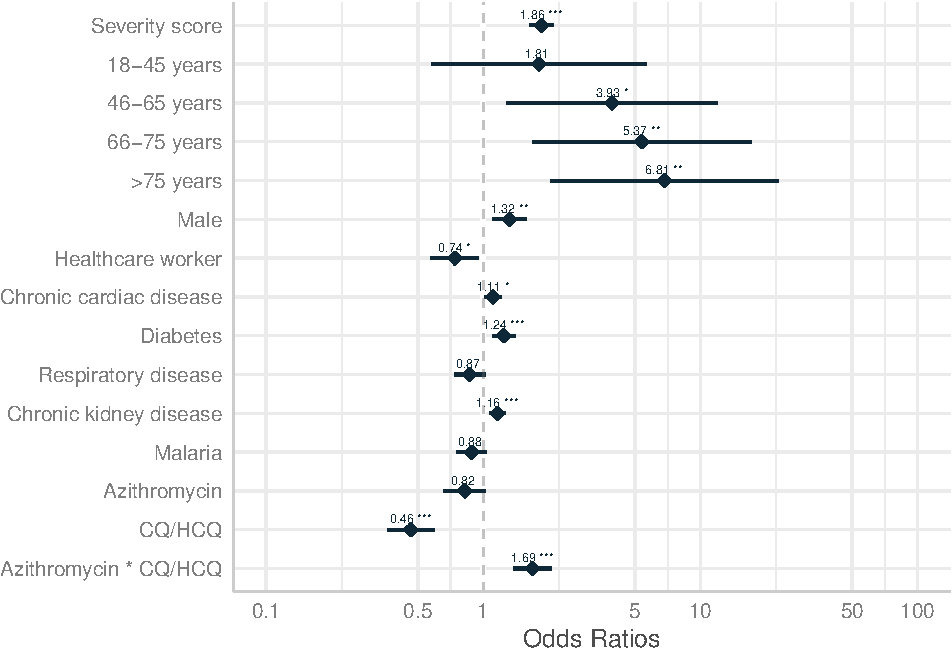
\includegraphics{results_files/figure-latex/forest-plot-1} 

}

\caption{Forest plot of standardized model coefficients}\label{fig:forest-plot}
\end{figure}

There is an interaction effect of azithromycin and chloroquine. There is
an interaction of azithromycin on the effect of chloroquine (see Figure
\ref{fig:interaction-plot}). There appears to be a blunting of the
effect of chloroquine on mortality by azithromycin. The predicted
probability of mortality in those who did not receive
chloroquine/hydroxychloroquine or azithromycin was 1.9\% compared to
0.6\% for those who received only azithromycin. This contrasted with a
predicted probability of mortality in those who received only
chloroquine/hydroxychloroquine of 0.1\% compared to 0.4\% for those who
received both chloroquine/hydroxychloroquine and azithromycin. In other
words, taking only chloroquine/hydroxychloroquine was associated with a
lower probability of mortality than taking both
chloroquine/hydroxychloroquine and azithromycin despite there being an
association with lower mortality with both drugs alone. However, it
should be noted that the size of this interaction effect is small and
unlikely to be clinically meaningful. It may not be reproducible and it
may be a spurious finding arising as a result of unknown patient or
study site characteristics, although we tried to account for site
effects by including site as a random effect in the regression model.

\begin{figure}[h]

{\centering 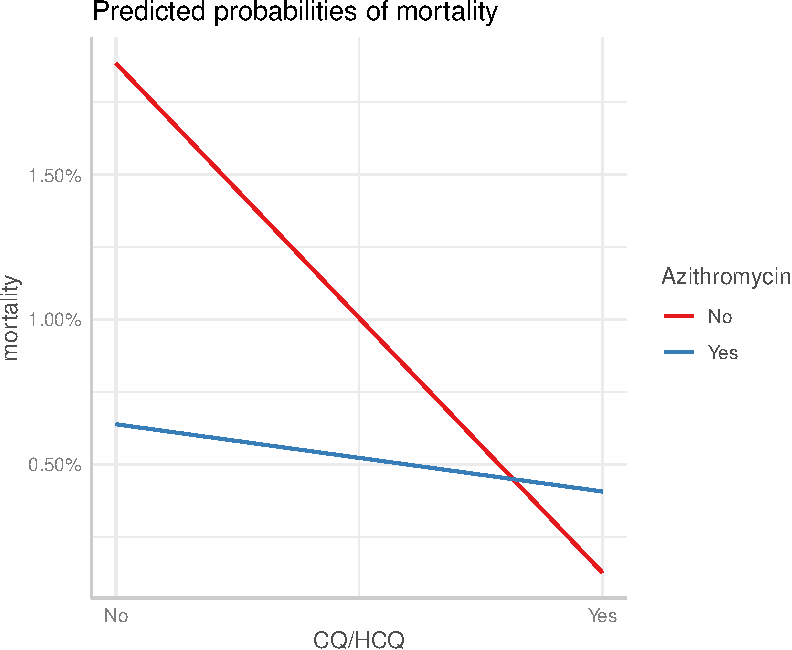
\includegraphics{results_files/figure-latex/interaction-plot-1} 

}

\caption{Interaction between azithromycin and chloroquine}\label{fig:interaction-plot}
\end{figure}

\clearpage

\hypertarget{cox-regression-model}{%
\subsection{Cox regression model}\label{cox-regression-model}}

 
  \providecommand{\huxb}[2]{\arrayrulecolor[RGB]{#1}\global\arrayrulewidth=#2pt}
  \providecommand{\huxvb}[2]{\color[RGB]{#1}\vrule width #2pt}
  \providecommand{\huxtpad}[1]{\rule{0pt}{#1}}
  \providecommand{\huxbpad}[1]{\rule[-#1]{0pt}{#1}}

\begin{table}[ht]
\begin{centerbox}
\begin{threeparttable}
\captionsetup{justification=centering,singlelinecheck=off}
\caption{Mixed effects cox regression model of predictors of time to mortality}
 \label{tab:cox-regression}
\setlength{\tabcolsep}{0pt}
\begin{tabularx}{0.96\textwidth}{p{0.48\textwidth} p{0.192\textwidth} p{0.192\textwidth} p{0.096\textwidth}}


\hhline{>{\huxb{0, 0, 0}{0.4}}->{\huxb{0, 0, 0}{0.4}}->{\huxb{0, 0, 0}{0.4}}->{\huxb{0, 0, 0}{0.4}}-}
\arrayrulecolor{black}

\multicolumn{1}{!{\huxvb{0, 0, 0}{0}}p{0.48\textwidth}!{\huxvb{0, 0, 0}{0}}}{\cellcolor[RGB]{255, 255, 255}\hspace{6pt}\parbox[b]{0.48\textwidth-6pt-6pt}{\huxtpad{1pt + 1em}\raggedright \textbf{{\fontsize{8pt}{9.6pt}\selectfont Predictors}}\huxbpad{1pt}}} &
\multicolumn{1}{p{0.192\textwidth}!{\huxvb{0, 0, 0}{0}}}{\cellcolor[RGB]{255, 255, 255}\hspace{6pt}\parbox[b]{0.192\textwidth-6pt-6pt}{\huxtpad{1pt + 1em}\raggedleft \textbf{{\fontsize{8pt}{9.6pt}\selectfont HR\hphantom{0}\hphantom{0}\hphantom{0}}}\huxbpad{1pt}}} &
\multicolumn{1}{p{0.192\textwidth}!{\huxvb{0, 0, 0}{0}}}{\cellcolor[RGB]{255, 255, 255}\hspace{6pt}\parbox[b]{0.192\textwidth-6pt-6pt}{\huxtpad{1pt + 1em}\centering \textbf{{\fontsize{8pt}{9.6pt}\selectfont 95\% CI}}\huxbpad{1pt}}} &
\multicolumn{1}{p{0.096\textwidth}!{\huxvb{0, 0, 0}{0}}}{\cellcolor[RGB]{255, 255, 255}\hspace{6pt}\parbox[b]{0.096\textwidth-6pt-6pt}{\huxtpad{1pt + 1em}\raggedleft \textbf{{\fontsize{8pt}{9.6pt}\selectfont p value}}\huxbpad{1pt}}} \tabularnewline[-0.5pt]


\hhline{>{\huxb{0, 0, 0}{0.4}}->{\huxb{0, 0, 0}{0.4}}->{\huxb{0, 0, 0}{0.4}}->{\huxb{0, 0, 0}{0.4}}-}
\arrayrulecolor{black}

\multicolumn{1}{!{\huxvb{0, 0, 0}{0}}p{0.48\textwidth}!{\huxvb{0, 0, 0}{0}}}{\cellcolor[RGB]{240, 240, 240}\hspace{6pt}\parbox[b]{0.48\textwidth-6pt-6pt}{\huxtpad{1pt + 1em}\raggedright {\fontsize{8pt}{9.6pt}\selectfont Severity score}\huxbpad{1pt}}} &
\multicolumn{1}{p{0.192\textwidth}!{\huxvb{0, 0, 0}{0}}}{\cellcolor[RGB]{240, 240, 240}\hspace{6pt}\parbox[b]{0.192\textwidth-6pt-6pt}{\huxtpad{1pt + 1em}\raggedleft {\fontsize{8pt}{9.6pt}\selectfont 2.57}\huxbpad{1pt}}} &
\multicolumn{1}{p{0.192\textwidth}!{\huxvb{0, 0, 0}{0}}}{\cellcolor[RGB]{240, 240, 240}\hspace{6pt}\parbox[b]{0.192\textwidth-6pt-6pt}{\huxtpad{1pt + 1em}\centering {\fontsize{8pt}{9.6pt}\selectfont 2.11,  3.12}\huxbpad{1pt}}} &
\multicolumn{1}{p{0.096\textwidth}!{\huxvb{0, 0, 0}{0}}}{\cellcolor[RGB]{240, 240, 240}\hspace{6pt}\parbox[b]{0.096\textwidth-6pt-6pt}{\huxtpad{1pt + 1em}\raggedleft {\fontsize{8pt}{9.6pt}\selectfont $<$0.001}\huxbpad{1pt}}} \tabularnewline[-0.5pt]


\hhline{}
\arrayrulecolor{black}

\multicolumn{1}{!{\huxvb{0, 0, 0}{0}}p{0.48\textwidth}!{\huxvb{0, 0, 0}{0}}}{\cellcolor[RGB]{255, 255, 255}\hspace{6pt}\parbox[b]{0.48\textwidth-6pt-6pt}{\huxtpad{1pt + 1em}\raggedright {\fontsize{8pt}{9.6pt}\selectfont Age group}\huxbpad{1pt}}} &
\multicolumn{1}{p{0.192\textwidth}!{\huxvb{0, 0, 0}{0}}}{\cellcolor[RGB]{255, 255, 255}\hspace{6pt}\parbox[b]{0.192\textwidth-6pt-6pt}{\huxtpad{1pt + 1em}\raggedleft {\fontsize{8pt}{9.6pt}\selectfont \hphantom{0}\hphantom{0}\hphantom{0}}\huxbpad{1pt}}} &
\multicolumn{1}{p{0.192\textwidth}!{\huxvb{0, 0, 0}{0}}}{\cellcolor[RGB]{255, 255, 255}\hspace{6pt}\parbox[b]{0.192\textwidth-6pt-6pt}{\huxtpad{1pt + 1em}\centering {\fontsize{8pt}{9.6pt}\selectfont }\huxbpad{1pt}}} &
\multicolumn{1}{p{0.096\textwidth}!{\huxvb{0, 0, 0}{0}}}{\cellcolor[RGB]{255, 255, 255}\hspace{6pt}\parbox[b]{0.096\textwidth-6pt-6pt}{\huxtpad{1pt + 1em}\raggedleft {\fontsize{8pt}{9.6pt}\selectfont }\huxbpad{1pt}}} \tabularnewline[-0.5pt]


\hhline{}
\arrayrulecolor{black}

\multicolumn{1}{!{\huxvb{0, 0, 0}{0}}p{0.48\textwidth}!{\huxvb{0, 0, 0}{0}}}{\cellcolor[RGB]{240, 240, 240}\hspace{6pt}\parbox[b]{0.48\textwidth-6pt-6pt}{\huxtpad{1pt + 1em}\raggedright {\fontsize{8pt}{9.6pt}\selectfont    $<$18}\huxbpad{1pt}}} &
\multicolumn{1}{p{0.192\textwidth}!{\huxvb{0, 0, 0}{0}}}{\cellcolor[RGB]{240, 240, 240}\hspace{6pt}\parbox[b]{0.192\textwidth-6pt-6pt}{\huxtpad{1pt + 1em}\raggedleft {\fontsize{8pt}{9.6pt}\selectfont ...\hphantom{0}\hphantom{0}}\huxbpad{1pt}}} &
\multicolumn{1}{p{0.192\textwidth}!{\huxvb{0, 0, 0}{0}}}{\cellcolor[RGB]{240, 240, 240}\hspace{6pt}\parbox[b]{0.192\textwidth-6pt-6pt}{\huxtpad{1pt + 1em}\centering {\fontsize{8pt}{9.6pt}\selectfont ...}\huxbpad{1pt}}} &
\multicolumn{1}{p{0.096\textwidth}!{\huxvb{0, 0, 0}{0}}}{\cellcolor[RGB]{240, 240, 240}\hspace{6pt}\parbox[b]{0.096\textwidth-6pt-6pt}{\huxtpad{1pt + 1em}\raggedleft {\fontsize{8pt}{9.6pt}\selectfont }\huxbpad{1pt}}} \tabularnewline[-0.5pt]


\hhline{}
\arrayrulecolor{black}

\multicolumn{1}{!{\huxvb{0, 0, 0}{0}}p{0.48\textwidth}!{\huxvb{0, 0, 0}{0}}}{\cellcolor[RGB]{255, 255, 255}\hspace{6pt}\parbox[b]{0.48\textwidth-6pt-6pt}{\huxtpad{1pt + 1em}\raggedright {\fontsize{8pt}{9.6pt}\selectfont    18$-$45}\huxbpad{1pt}}} &
\multicolumn{1}{p{0.192\textwidth}!{\huxvb{0, 0, 0}{0}}}{\cellcolor[RGB]{255, 255, 255}\hspace{6pt}\parbox[b]{0.192\textwidth-6pt-6pt}{\huxtpad{1pt + 1em}\raggedleft {\fontsize{8pt}{9.6pt}\selectfont 1.47}\huxbpad{1pt}}} &
\multicolumn{1}{p{0.192\textwidth}!{\huxvb{0, 0, 0}{0}}}{\cellcolor[RGB]{255, 255, 255}\hspace{6pt}\parbox[b]{0.192\textwidth-6pt-6pt}{\huxtpad{1pt + 1em}\centering {\fontsize{8pt}{9.6pt}\selectfont 0.44,  4.95}\huxbpad{1pt}}} &
\multicolumn{1}{p{0.096\textwidth}!{\huxvb{0, 0, 0}{0}}}{\cellcolor[RGB]{255, 255, 255}\hspace{6pt}\parbox[b]{0.096\textwidth-6pt-6pt}{\huxtpad{1pt + 1em}\raggedleft {\fontsize{8pt}{9.6pt}\selectfont 0.531}\huxbpad{1pt}}} \tabularnewline[-0.5pt]


\hhline{}
\arrayrulecolor{black}

\multicolumn{1}{!{\huxvb{0, 0, 0}{0}}p{0.48\textwidth}!{\huxvb{0, 0, 0}{0}}}{\cellcolor[RGB]{240, 240, 240}\hspace{6pt}\parbox[b]{0.48\textwidth-6pt-6pt}{\huxtpad{1pt + 1em}\raggedright {\fontsize{8pt}{9.6pt}\selectfont    46$-$65}\huxbpad{1pt}}} &
\multicolumn{1}{p{0.192\textwidth}!{\huxvb{0, 0, 0}{0}}}{\cellcolor[RGB]{240, 240, 240}\hspace{6pt}\parbox[b]{0.192\textwidth-6pt-6pt}{\huxtpad{1pt + 1em}\raggedleft {\fontsize{8pt}{9.6pt}\selectfont 2.66}\huxbpad{1pt}}} &
\multicolumn{1}{p{0.192\textwidth}!{\huxvb{0, 0, 0}{0}}}{\cellcolor[RGB]{240, 240, 240}\hspace{6pt}\parbox[b]{0.192\textwidth-6pt-6pt}{\huxtpad{1pt + 1em}\centering {\fontsize{8pt}{9.6pt}\selectfont 0.82,  8.66}\huxbpad{1pt}}} &
\multicolumn{1}{p{0.096\textwidth}!{\huxvb{0, 0, 0}{0}}}{\cellcolor[RGB]{240, 240, 240}\hspace{6pt}\parbox[b]{0.096\textwidth-6pt-6pt}{\huxtpad{1pt + 1em}\raggedleft {\fontsize{8pt}{9.6pt}\selectfont 0.104}\huxbpad{1pt}}} \tabularnewline[-0.5pt]


\hhline{}
\arrayrulecolor{black}

\multicolumn{1}{!{\huxvb{0, 0, 0}{0}}p{0.48\textwidth}!{\huxvb{0, 0, 0}{0}}}{\cellcolor[RGB]{255, 255, 255}\hspace{6pt}\parbox[b]{0.48\textwidth-6pt-6pt}{\huxtpad{1pt + 1em}\raggedright {\fontsize{8pt}{9.6pt}\selectfont    66$-$75}\huxbpad{1pt}}} &
\multicolumn{1}{p{0.192\textwidth}!{\huxvb{0, 0, 0}{0}}}{\cellcolor[RGB]{255, 255, 255}\hspace{6pt}\parbox[b]{0.192\textwidth-6pt-6pt}{\huxtpad{1pt + 1em}\raggedleft {\fontsize{8pt}{9.6pt}\selectfont 3.54}\huxbpad{1pt}}} &
\multicolumn{1}{p{0.192\textwidth}!{\huxvb{0, 0, 0}{0}}}{\cellcolor[RGB]{255, 255, 255}\hspace{6pt}\parbox[b]{0.192\textwidth-6pt-6pt}{\huxtpad{1pt + 1em}\centering {\fontsize{8pt}{9.6pt}\selectfont 1.06, 11.83}\huxbpad{1pt}}} &
\multicolumn{1}{p{0.096\textwidth}!{\huxvb{0, 0, 0}{0}}}{\cellcolor[RGB]{255, 255, 255}\hspace{6pt}\parbox[b]{0.096\textwidth-6pt-6pt}{\huxtpad{1pt + 1em}\raggedleft {\fontsize{8pt}{9.6pt}\selectfont 0.040}\huxbpad{1pt}}} \tabularnewline[-0.5pt]


\hhline{}
\arrayrulecolor{black}

\multicolumn{1}{!{\huxvb{0, 0, 0}{0}}p{0.48\textwidth}!{\huxvb{0, 0, 0}{0}}}{\cellcolor[RGB]{240, 240, 240}\hspace{6pt}\parbox[b]{0.48\textwidth-6pt-6pt}{\huxtpad{1pt + 1em}\raggedright {\fontsize{8pt}{9.6pt}\selectfont    $>$75}\huxbpad{1pt}}} &
\multicolumn{1}{p{0.192\textwidth}!{\huxvb{0, 0, 0}{0}}}{\cellcolor[RGB]{240, 240, 240}\hspace{6pt}\parbox[b]{0.192\textwidth-6pt-6pt}{\huxtpad{1pt + 1em}\raggedleft {\fontsize{8pt}{9.6pt}\selectfont 3.58}\huxbpad{1pt}}} &
\multicolumn{1}{p{0.192\textwidth}!{\huxvb{0, 0, 0}{0}}}{\cellcolor[RGB]{240, 240, 240}\hspace{6pt}\parbox[b]{0.192\textwidth-6pt-6pt}{\huxtpad{1pt + 1em}\centering {\fontsize{8pt}{9.6pt}\selectfont 1.05, 12.15}\huxbpad{1pt}}} &
\multicolumn{1}{p{0.096\textwidth}!{\huxvb{0, 0, 0}{0}}}{\cellcolor[RGB]{240, 240, 240}\hspace{6pt}\parbox[b]{0.096\textwidth-6pt-6pt}{\huxtpad{1pt + 1em}\raggedleft {\fontsize{8pt}{9.6pt}\selectfont 0.041}\huxbpad{1pt}}} \tabularnewline[-0.5pt]


\hhline{}
\arrayrulecolor{black}

\multicolumn{1}{!{\huxvb{0, 0, 0}{0}}p{0.48\textwidth}!{\huxvb{0, 0, 0}{0}}}{\cellcolor[RGB]{255, 255, 255}\hspace{6pt}\parbox[b]{0.48\textwidth-6pt-6pt}{\huxtpad{1pt + 1em}\raggedright {\fontsize{8pt}{9.6pt}\selectfont Male}\huxbpad{1pt}}} &
\multicolumn{1}{p{0.192\textwidth}!{\huxvb{0, 0, 0}{0}}}{\cellcolor[RGB]{255, 255, 255}\hspace{6pt}\parbox[b]{0.192\textwidth-6pt-6pt}{\huxtpad{1pt + 1em}\raggedleft {\fontsize{8pt}{9.6pt}\selectfont 1.66}\huxbpad{1pt}}} &
\multicolumn{1}{p{0.192\textwidth}!{\huxvb{0, 0, 0}{0}}}{\cellcolor[RGB]{255, 255, 255}\hspace{6pt}\parbox[b]{0.192\textwidth-6pt-6pt}{\huxtpad{1pt + 1em}\centering {\fontsize{8pt}{9.6pt}\selectfont 1.19,  2.32}\huxbpad{1pt}}} &
\multicolumn{1}{p{0.096\textwidth}!{\huxvb{0, 0, 0}{0}}}{\cellcolor[RGB]{255, 255, 255}\hspace{6pt}\parbox[b]{0.096\textwidth-6pt-6pt}{\huxtpad{1pt + 1em}\raggedleft {\fontsize{8pt}{9.6pt}\selectfont 0.003}\huxbpad{1pt}}} \tabularnewline[-0.5pt]


\hhline{}
\arrayrulecolor{black}

\multicolumn{1}{!{\huxvb{0, 0, 0}{0}}p{0.48\textwidth}!{\huxvb{0, 0, 0}{0}}}{\cellcolor[RGB]{240, 240, 240}\hspace{6pt}\parbox[b]{0.48\textwidth-6pt-6pt}{\huxtpad{1pt + 1em}\raggedright {\fontsize{8pt}{9.6pt}\selectfont Health care worker}\huxbpad{1pt}}} &
\multicolumn{1}{p{0.192\textwidth}!{\huxvb{0, 0, 0}{0}}}{\cellcolor[RGB]{240, 240, 240}\hspace{6pt}\parbox[b]{0.192\textwidth-6pt-6pt}{\huxtpad{1pt + 1em}\raggedleft {\fontsize{8pt}{9.6pt}\selectfont 0.35}\huxbpad{1pt}}} &
\multicolumn{1}{p{0.192\textwidth}!{\huxvb{0, 0, 0}{0}}}{\cellcolor[RGB]{240, 240, 240}\hspace{6pt}\parbox[b]{0.192\textwidth-6pt-6pt}{\huxtpad{1pt + 1em}\centering {\fontsize{8pt}{9.6pt}\selectfont 0.11,  1.13}\huxbpad{1pt}}} &
\multicolumn{1}{p{0.096\textwidth}!{\huxvb{0, 0, 0}{0}}}{\cellcolor[RGB]{240, 240, 240}\hspace{6pt}\parbox[b]{0.096\textwidth-6pt-6pt}{\huxtpad{1pt + 1em}\raggedleft {\fontsize{8pt}{9.6pt}\selectfont 0.079}\huxbpad{1pt}}} \tabularnewline[-0.5pt]


\hhline{}
\arrayrulecolor{black}

\multicolumn{1}{!{\huxvb{0, 0, 0}{0}}p{0.48\textwidth}!{\huxvb{0, 0, 0}{0}}}{\cellcolor[RGB]{255, 255, 255}\hspace{6pt}\parbox[b]{0.48\textwidth-6pt-6pt}{\huxtpad{1pt + 1em}\raggedright {\fontsize{8pt}{9.6pt}\selectfont Chronic cardiac disease (not hypertension)}\huxbpad{1pt}}} &
\multicolumn{1}{p{0.192\textwidth}!{\huxvb{0, 0, 0}{0}}}{\cellcolor[RGB]{255, 255, 255}\hspace{6pt}\parbox[b]{0.192\textwidth-6pt-6pt}{\huxtpad{1pt + 1em}\raggedleft {\fontsize{8pt}{9.6pt}\selectfont 2.34}\huxbpad{1pt}}} &
\multicolumn{1}{p{0.192\textwidth}!{\huxvb{0, 0, 0}{0}}}{\cellcolor[RGB]{255, 255, 255}\hspace{6pt}\parbox[b]{0.192\textwidth-6pt-6pt}{\huxtpad{1pt + 1em}\centering {\fontsize{8pt}{9.6pt}\selectfont 1.22,  4.48}\huxbpad{1pt}}} &
\multicolumn{1}{p{0.096\textwidth}!{\huxvb{0, 0, 0}{0}}}{\cellcolor[RGB]{255, 255, 255}\hspace{6pt}\parbox[b]{0.096\textwidth-6pt-6pt}{\huxtpad{1pt + 1em}\raggedleft {\fontsize{8pt}{9.6pt}\selectfont 0.010}\huxbpad{1pt}}} \tabularnewline[-0.5pt]


\hhline{}
\arrayrulecolor{black}

\multicolumn{1}{!{\huxvb{0, 0, 0}{0}}p{0.48\textwidth}!{\huxvb{0, 0, 0}{0}}}{\cellcolor[RGB]{240, 240, 240}\hspace{6pt}\parbox[b]{0.48\textwidth-6pt-6pt}{\huxtpad{1pt + 1em}\raggedright {\fontsize{8pt}{9.6pt}\selectfont Diabetes}\huxbpad{1pt}}} &
\multicolumn{1}{p{0.192\textwidth}!{\huxvb{0, 0, 0}{0}}}{\cellcolor[RGB]{240, 240, 240}\hspace{6pt}\parbox[b]{0.192\textwidth-6pt-6pt}{\huxtpad{1pt + 1em}\raggedleft {\fontsize{8pt}{9.6pt}\selectfont 1.99}\huxbpad{1pt}}} &
\multicolumn{1}{p{0.192\textwidth}!{\huxvb{0, 0, 0}{0}}}{\cellcolor[RGB]{240, 240, 240}\hspace{6pt}\parbox[b]{0.192\textwidth-6pt-6pt}{\huxtpad{1pt + 1em}\centering {\fontsize{8pt}{9.6pt}\selectfont 1.41,  2.80}\huxbpad{1pt}}} &
\multicolumn{1}{p{0.096\textwidth}!{\huxvb{0, 0, 0}{0}}}{\cellcolor[RGB]{240, 240, 240}\hspace{6pt}\parbox[b]{0.096\textwidth-6pt-6pt}{\huxtpad{1pt + 1em}\raggedleft {\fontsize{8pt}{9.6pt}\selectfont $<$0.001}\huxbpad{1pt}}} \tabularnewline[-0.5pt]


\hhline{}
\arrayrulecolor{black}

\multicolumn{1}{!{\huxvb{0, 0, 0}{0}}p{0.48\textwidth}!{\huxvb{0, 0, 0}{0}}}{\cellcolor[RGB]{255, 255, 255}\hspace{6pt}\parbox[b]{0.48\textwidth-6pt-6pt}{\huxtpad{1pt + 1em}\raggedright {\fontsize{8pt}{9.6pt}\selectfont Respiratory disease}\huxbpad{1pt}}} &
\multicolumn{1}{p{0.192\textwidth}!{\huxvb{0, 0, 0}{0}}}{\cellcolor[RGB]{255, 255, 255}\hspace{6pt}\parbox[b]{0.192\textwidth-6pt-6pt}{\huxtpad{1pt + 1em}\raggedleft {\fontsize{8pt}{9.6pt}\selectfont 0.29}\huxbpad{1pt}}} &
\multicolumn{1}{p{0.192\textwidth}!{\huxvb{0, 0, 0}{0}}}{\cellcolor[RGB]{255, 255, 255}\hspace{6pt}\parbox[b]{0.192\textwidth-6pt-6pt}{\huxtpad{1pt + 1em}\centering {\fontsize{8pt}{9.6pt}\selectfont 0.09,  0.94}\huxbpad{1pt}}} &
\multicolumn{1}{p{0.096\textwidth}!{\huxvb{0, 0, 0}{0}}}{\cellcolor[RGB]{255, 255, 255}\hspace{6pt}\parbox[b]{0.096\textwidth-6pt-6pt}{\huxtpad{1pt + 1em}\raggedleft {\fontsize{8pt}{9.6pt}\selectfont 0.039}\huxbpad{1pt}}} \tabularnewline[-0.5pt]


\hhline{}
\arrayrulecolor{black}

\multicolumn{1}{!{\huxvb{0, 0, 0}{0}}p{0.48\textwidth}!{\huxvb{0, 0, 0}{0}}}{\cellcolor[RGB]{240, 240, 240}\hspace{6pt}\parbox[b]{0.48\textwidth-6pt-6pt}{\huxtpad{1pt + 1em}\raggedright {\fontsize{8pt}{9.6pt}\selectfont Chronic kidney disease}\huxbpad{1pt}}} &
\multicolumn{1}{p{0.192\textwidth}!{\huxvb{0, 0, 0}{0}}}{\cellcolor[RGB]{240, 240, 240}\hspace{6pt}\parbox[b]{0.192\textwidth-6pt-6pt}{\huxtpad{1pt + 1em}\raggedleft {\fontsize{8pt}{9.6pt}\selectfont 8.21}\huxbpad{1pt}}} &
\multicolumn{1}{p{0.192\textwidth}!{\huxvb{0, 0, 0}{0}}}{\cellcolor[RGB]{240, 240, 240}\hspace{6pt}\parbox[b]{0.192\textwidth-6pt-6pt}{\huxtpad{1pt + 1em}\centering {\fontsize{8pt}{9.6pt}\selectfont 2.86, 23.56}\huxbpad{1pt}}} &
\multicolumn{1}{p{0.096\textwidth}!{\huxvb{0, 0, 0}{0}}}{\cellcolor[RGB]{240, 240, 240}\hspace{6pt}\parbox[b]{0.096\textwidth-6pt-6pt}{\huxtpad{1pt + 1em}\raggedleft {\fontsize{8pt}{9.6pt}\selectfont $<$0.001}\huxbpad{1pt}}} \tabularnewline[-0.5pt]


\hhline{}
\arrayrulecolor{black}

\multicolumn{1}{!{\huxvb{0, 0, 0}{0}}p{0.48\textwidth}!{\huxvb{0, 0, 0}{0}}}{\cellcolor[RGB]{255, 255, 255}\hspace{6pt}\parbox[b]{0.48\textwidth-6pt-6pt}{\huxtpad{1pt + 1em}\raggedright {\fontsize{8pt}{9.6pt}\selectfont Malaria}\huxbpad{1pt}}} &
\multicolumn{1}{p{0.192\textwidth}!{\huxvb{0, 0, 0}{0}}}{\cellcolor[RGB]{255, 255, 255}\hspace{6pt}\parbox[b]{0.192\textwidth-6pt-6pt}{\huxtpad{1pt + 1em}\raggedleft {\fontsize{8pt}{9.6pt}\selectfont 0.42}\huxbpad{1pt}}} &
\multicolumn{1}{p{0.192\textwidth}!{\huxvb{0, 0, 0}{0}}}{\cellcolor[RGB]{255, 255, 255}\hspace{6pt}\parbox[b]{0.192\textwidth-6pt-6pt}{\huxtpad{1pt + 1em}\centering {\fontsize{8pt}{9.6pt}\selectfont 0.15,  1.20}\huxbpad{1pt}}} &
\multicolumn{1}{p{0.096\textwidth}!{\huxvb{0, 0, 0}{0}}}{\cellcolor[RGB]{255, 255, 255}\hspace{6pt}\parbox[b]{0.096\textwidth-6pt-6pt}{\huxtpad{1pt + 1em}\raggedleft {\fontsize{8pt}{9.6pt}\selectfont 0.104}\huxbpad{1pt}}} \tabularnewline[-0.5pt]


\hhline{}
\arrayrulecolor{black}

\multicolumn{1}{!{\huxvb{0, 0, 0}{0}}p{0.48\textwidth}!{\huxvb{0, 0, 0}{0}}}{\cellcolor[RGB]{240, 240, 240}\hspace{6pt}\parbox[b]{0.48\textwidth-6pt-6pt}{\huxtpad{1pt + 1em}\raggedright {\fontsize{8pt}{9.6pt}\selectfont Azithromycin}\huxbpad{1pt}}} &
\multicolumn{1}{p{0.192\textwidth}!{\huxvb{0, 0, 0}{0}}}{\cellcolor[RGB]{240, 240, 240}\hspace{6pt}\parbox[b]{0.192\textwidth-6pt-6pt}{\huxtpad{1pt + 1em}\raggedleft {\fontsize{8pt}{9.6pt}\selectfont 0.55}\huxbpad{1pt}}} &
\multicolumn{1}{p{0.192\textwidth}!{\huxvb{0, 0, 0}{0}}}{\cellcolor[RGB]{240, 240, 240}\hspace{6pt}\parbox[b]{0.192\textwidth-6pt-6pt}{\huxtpad{1pt + 1em}\centering {\fontsize{8pt}{9.6pt}\selectfont 0.35,  0.86}\huxbpad{1pt}}} &
\multicolumn{1}{p{0.096\textwidth}!{\huxvb{0, 0, 0}{0}}}{\cellcolor[RGB]{240, 240, 240}\hspace{6pt}\parbox[b]{0.096\textwidth-6pt-6pt}{\huxtpad{1pt + 1em}\raggedleft {\fontsize{8pt}{9.6pt}\selectfont 0.008}\huxbpad{1pt}}} \tabularnewline[-0.5pt]


\hhline{}
\arrayrulecolor{black}

\multicolumn{1}{!{\huxvb{0, 0, 0}{0}}p{0.48\textwidth}!{\huxvb{0, 0, 0}{0}}}{\cellcolor[RGB]{255, 255, 255}\hspace{6pt}\parbox[b]{0.48\textwidth-6pt-6pt}{\huxtpad{1pt + 1em}\raggedright {\fontsize{8pt}{9.6pt}\selectfont CQ/HCQ}\huxbpad{1pt}}} &
\multicolumn{1}{p{0.192\textwidth}!{\huxvb{0, 0, 0}{0}}}{\cellcolor[RGB]{255, 255, 255}\hspace{6pt}\parbox[b]{0.192\textwidth-6pt-6pt}{\huxtpad{1pt + 1em}\raggedleft {\fontsize{8pt}{9.6pt}\selectfont 0.20}\huxbpad{1pt}}} &
\multicolumn{1}{p{0.192\textwidth}!{\huxvb{0, 0, 0}{0}}}{\cellcolor[RGB]{255, 255, 255}\hspace{6pt}\parbox[b]{0.192\textwidth-6pt-6pt}{\huxtpad{1pt + 1em}\centering {\fontsize{8pt}{9.6pt}\selectfont 0.10,  0.38}\huxbpad{1pt}}} &
\multicolumn{1}{p{0.096\textwidth}!{\huxvb{0, 0, 0}{0}}}{\cellcolor[RGB]{255, 255, 255}\hspace{6pt}\parbox[b]{0.096\textwidth-6pt-6pt}{\huxtpad{1pt + 1em}\raggedleft {\fontsize{8pt}{9.6pt}\selectfont $<$0.001}\huxbpad{1pt}}} \tabularnewline[-0.5pt]


\hhline{}
\arrayrulecolor{black}

\multicolumn{1}{!{\huxvb{0, 0, 0}{0}}p{0.48\textwidth}!{\huxvb{0, 0, 0}{0}}}{\cellcolor[RGB]{240, 240, 240}\hspace{6pt}\parbox[b]{0.48\textwidth-6pt-6pt}{\huxtpad{1pt + 1em}\raggedright {\fontsize{8pt}{9.6pt}\selectfont Azithromycin * CQ/HCQ}\huxbpad{1pt}}} &
\multicolumn{1}{p{0.192\textwidth}!{\huxvb{0, 0, 0}{0}}}{\cellcolor[RGB]{240, 240, 240}\hspace{6pt}\parbox[b]{0.192\textwidth-6pt-6pt}{\huxtpad{1pt + 1em}\raggedleft {\fontsize{8pt}{9.6pt}\selectfont 4.57}\huxbpad{1pt}}} &
\multicolumn{1}{p{0.192\textwidth}!{\huxvb{0, 0, 0}{0}}}{\cellcolor[RGB]{240, 240, 240}\hspace{6pt}\parbox[b]{0.192\textwidth-6pt-6pt}{\huxtpad{1pt + 1em}\centering {\fontsize{8pt}{9.6pt}\selectfont 2.12,  9.85}\huxbpad{1pt}}} &
\multicolumn{1}{p{0.096\textwidth}!{\huxvb{0, 0, 0}{0}}}{\cellcolor[RGB]{240, 240, 240}\hspace{6pt}\parbox[b]{0.096\textwidth-6pt-6pt}{\huxtpad{1pt + 1em}\raggedleft {\fontsize{8pt}{9.6pt}\selectfont $<$0.001}\huxbpad{1pt}}} \tabularnewline[-0.5pt]


\hhline{}
\arrayrulecolor{black}

\multicolumn{1}{!{\huxvb{0, 0, 0}{0}}p{0.48\textwidth}!{\huxvb{0, 0, 0}{0}}}{\cellcolor[RGB]{255, 255, 255}\hspace{6pt}\parbox[b]{0.48\textwidth-6pt-6pt}{\huxtpad{1pt + 1em}\raggedright {\fontsize{8pt}{9.6pt}\selectfont }\huxbpad{1pt}}} &
\multicolumn{1}{p{0.192\textwidth}!{\huxvb{0, 0, 0}{0}}}{\cellcolor[RGB]{255, 255, 255}\hspace{6pt}\parbox[b]{0.192\textwidth-6pt-6pt}{\huxtpad{1pt + 1em}\raggedleft {\fontsize{8pt}{9.6pt}\selectfont \hphantom{0}\hphantom{0}\hphantom{0}}\huxbpad{1pt}}} &
\multicolumn{1}{p{0.192\textwidth}!{\huxvb{0, 0, 0}{0}}}{\cellcolor[RGB]{255, 255, 255}\hspace{6pt}\parbox[b]{0.192\textwidth-6pt-6pt}{\huxtpad{1pt + 1em}\centering {\fontsize{8pt}{9.6pt}\selectfont }\huxbpad{1pt}}} &
\multicolumn{1}{p{0.096\textwidth}!{\huxvb{0, 0, 0}{0}}}{\cellcolor[RGB]{255, 255, 255}\hspace{6pt}\parbox[b]{0.096\textwidth-6pt-6pt}{\huxtpad{1pt + 1em}\raggedleft {\fontsize{8pt}{9.6pt}\selectfont }\huxbpad{1pt}}} \tabularnewline[-0.5pt]


\hhline{}
\arrayrulecolor{black}

\multicolumn{1}{!{\huxvb{0, 0, 0}{0}}p{0.48\textwidth}!{\huxvb{0, 0, 0}{0}}}{\cellcolor[RGB]{240, 240, 240}\hspace{6pt}\parbox[b]{0.48\textwidth-6pt-6pt}{\huxtpad{1pt + 1em}\raggedright {\fontsize{8pt}{9.6pt}\selectfont Number of observations}\huxbpad{1pt}}} &
\multicolumn{1}{p{0.192\textwidth}!{\huxvb{0, 0, 0}{0}}}{\cellcolor[RGB]{240, 240, 240}\hspace{6pt}\parbox[b]{0.192\textwidth-6pt-6pt}{\huxtpad{1pt + 1em}\raggedleft {\fontsize{8pt}{9.6pt}\selectfont 3178\hphantom{0}\hphantom{0}\hphantom{0}}\huxbpad{1pt}}} &
\multicolumn{1}{p{0.192\textwidth}!{\huxvb{0, 0, 0}{0}}}{\cellcolor[RGB]{240, 240, 240}\hspace{6pt}\parbox[b]{0.192\textwidth-6pt-6pt}{\huxtpad{1pt + 1em}\centering {\fontsize{8pt}{9.6pt}\selectfont }\huxbpad{1pt}}} &
\multicolumn{1}{p{0.096\textwidth}!{\huxvb{0, 0, 0}{0}}}{\cellcolor[RGB]{240, 240, 240}\hspace{6pt}\parbox[b]{0.096\textwidth-6pt-6pt}{\huxtpad{1pt + 1em}\raggedleft {\fontsize{8pt}{9.6pt}\selectfont }\huxbpad{1pt}}} \tabularnewline[-0.5pt]


\hhline{}
\arrayrulecolor{black}

\multicolumn{1}{!{\huxvb{0, 0, 0}{0}}p{0.48\textwidth}!{\huxvb{0, 0, 0}{0}}}{\cellcolor[RGB]{255, 255, 255}\hspace{6pt}\parbox[b]{0.48\textwidth-6pt-6pt}{\huxtpad{1pt + 1em}\raggedright {\fontsize{8pt}{9.6pt}\selectfont Number of events}\huxbpad{1pt}}} &
\multicolumn{1}{p{0.192\textwidth}!{\huxvb{0, 0, 0}{0}}}{\cellcolor[RGB]{255, 255, 255}\hspace{6pt}\parbox[b]{0.192\textwidth-6pt-6pt}{\huxtpad{1pt + 1em}\raggedleft {\fontsize{8pt}{9.6pt}\selectfont 192\hphantom{0}\hphantom{0}\hphantom{0}}\huxbpad{1pt}}} &
\multicolumn{1}{p{0.192\textwidth}!{\huxvb{0, 0, 0}{0}}}{\cellcolor[RGB]{255, 255, 255}\hspace{6pt}\parbox[b]{0.192\textwidth-6pt-6pt}{\huxtpad{1pt + 1em}\centering {\fontsize{8pt}{9.6pt}\selectfont }\huxbpad{1pt}}} &
\multicolumn{1}{p{0.096\textwidth}!{\huxvb{0, 0, 0}{0}}}{\cellcolor[RGB]{255, 255, 255}\hspace{6pt}\parbox[b]{0.096\textwidth-6pt-6pt}{\huxtpad{1pt + 1em}\raggedleft {\fontsize{8pt}{9.6pt}\selectfont }\huxbpad{1pt}}} \tabularnewline[-0.5pt]


\hhline{}
\arrayrulecolor{black}

\multicolumn{1}{!{\huxvb{0, 0, 0}{0}}p{0.48\textwidth}!{\huxvb{0, 0, 0}{0}}}{\cellcolor[RGB]{240, 240, 240}\hspace{6pt}\parbox[b]{0.48\textwidth-6pt-6pt}{\huxtpad{1pt + 1em}\raggedright {\fontsize{8pt}{9.6pt}\selectfont site σ²}\huxbpad{1pt}}} &
\multicolumn{1}{p{0.192\textwidth}!{\huxvb{0, 0, 0}{0}}}{\cellcolor[RGB]{240, 240, 240}\hspace{6pt}\parbox[b]{0.192\textwidth-6pt-6pt}{\huxtpad{1pt + 1em}\raggedleft {\fontsize{8pt}{9.6pt}\selectfont 0.56}\huxbpad{1pt}}} &
\multicolumn{1}{p{0.192\textwidth}!{\huxvb{0, 0, 0}{0}}}{\cellcolor[RGB]{240, 240, 240}\hspace{6pt}\parbox[b]{0.192\textwidth-6pt-6pt}{\huxtpad{1pt + 1em}\centering {\fontsize{8pt}{9.6pt}\selectfont }\huxbpad{1pt}}} &
\multicolumn{1}{p{0.096\textwidth}!{\huxvb{0, 0, 0}{0}}}{\cellcolor[RGB]{240, 240, 240}\hspace{6pt}\parbox[b]{0.096\textwidth-6pt-6pt}{\huxtpad{1pt + 1em}\raggedleft {\fontsize{8pt}{9.6pt}\selectfont }\huxbpad{1pt}}} \tabularnewline[-0.5pt]


\hhline{}
\arrayrulecolor{black}

\multicolumn{1}{!{\huxvb{0, 0, 0}{0}}p{0.48\textwidth}!{\huxvb{0, 0, 0}{0}}}{\cellcolor[RGB]{255, 255, 255}\hspace{6pt}\parbox[b]{0.48\textwidth-6pt-6pt}{\huxtpad{1pt + 1em}\raggedright {\fontsize{8pt}{9.6pt}\selectfont facility type σ²}\huxbpad{1pt}}} &
\multicolumn{1}{p{0.192\textwidth}!{\huxvb{0, 0, 0}{0}}}{\cellcolor[RGB]{255, 255, 255}\hspace{6pt}\parbox[b]{0.192\textwidth-6pt-6pt}{\huxtpad{1pt + 1em}\raggedleft {\fontsize{8pt}{9.6pt}\selectfont 1.51}\huxbpad{1pt}}} &
\multicolumn{1}{p{0.192\textwidth}!{\huxvb{0, 0, 0}{0}}}{\cellcolor[RGB]{255, 255, 255}\hspace{6pt}\parbox[b]{0.192\textwidth-6pt-6pt}{\huxtpad{1pt + 1em}\centering {\fontsize{8pt}{9.6pt}\selectfont }\huxbpad{1pt}}} &
\multicolumn{1}{p{0.096\textwidth}!{\huxvb{0, 0, 0}{0}}}{\cellcolor[RGB]{255, 255, 255}\hspace{6pt}\parbox[b]{0.096\textwidth-6pt-6pt}{\huxtpad{1pt + 1em}\raggedleft {\fontsize{8pt}{9.6pt}\selectfont }\huxbpad{1pt}}} \tabularnewline[-0.5pt]


\hhline{}
\arrayrulecolor{black}

\multicolumn{1}{!{\huxvb{0, 0, 0}{0}}p{0.48\textwidth}!{\huxvb{0, 0, 0}{0}}}{\cellcolor[RGB]{240, 240, 240}\hspace{6pt}\parbox[b]{0.48\textwidth-6pt-6pt}{\huxtpad{1pt + 1em}\raggedright {\fontsize{8pt}{9.6pt}\selectfont Log-likelihood}\huxbpad{1pt}}} &
\multicolumn{1}{p{0.192\textwidth}!{\huxvb{0, 0, 0}{0}}}{\cellcolor[RGB]{240, 240, 240}\hspace{6pt}\parbox[b]{0.192\textwidth-6pt-6pt}{\huxtpad{1pt + 1em}\raggedleft {\fontsize{8pt}{9.6pt}\selectfont $-$1156.94}\huxbpad{1pt}}} &
\multicolumn{1}{p{0.192\textwidth}!{\huxvb{0, 0, 0}{0}}}{\cellcolor[RGB]{240, 240, 240}\hspace{6pt}\parbox[b]{0.192\textwidth-6pt-6pt}{\huxtpad{1pt + 1em}\centering {\fontsize{8pt}{9.6pt}\selectfont }\huxbpad{1pt}}} &
\multicolumn{1}{p{0.096\textwidth}!{\huxvb{0, 0, 0}{0}}}{\cellcolor[RGB]{240, 240, 240}\hspace{6pt}\parbox[b]{0.096\textwidth-6pt-6pt}{\huxtpad{1pt + 1em}\raggedleft {\fontsize{8pt}{9.6pt}\selectfont }\huxbpad{1pt}}} \tabularnewline[-0.5pt]


\hhline{}
\arrayrulecolor{black}

\multicolumn{1}{!{\huxvb{0, 0, 0}{0}}p{0.48\textwidth}!{\huxvb{0, 0, 0}{0}}}{\cellcolor[RGB]{255, 255, 255}\hspace{6pt}\parbox[b]{0.48\textwidth-6pt-6pt}{\huxtpad{1pt + 1em}\raggedright {\fontsize{8pt}{9.6pt}\selectfont AIC}\huxbpad{1pt}}} &
\multicolumn{1}{p{0.192\textwidth}!{\huxvb{0, 0, 0}{0}}}{\cellcolor[RGB]{255, 255, 255}\hspace{6pt}\parbox[b]{0.192\textwidth-6pt-6pt}{\huxtpad{1pt + 1em}\raggedleft {\fontsize{8pt}{9.6pt}\selectfont 2367.52}\huxbpad{1pt}}} &
\multicolumn{1}{p{0.192\textwidth}!{\huxvb{0, 0, 0}{0}}}{\cellcolor[RGB]{255, 255, 255}\hspace{6pt}\parbox[b]{0.192\textwidth-6pt-6pt}{\huxtpad{1pt + 1em}\centering {\fontsize{8pt}{9.6pt}\selectfont }\huxbpad{1pt}}} &
\multicolumn{1}{p{0.096\textwidth}!{\huxvb{0, 0, 0}{0}}}{\cellcolor[RGB]{255, 255, 255}\hspace{6pt}\parbox[b]{0.096\textwidth-6pt-6pt}{\huxtpad{1pt + 1em}\raggedleft {\fontsize{8pt}{9.6pt}\selectfont }\huxbpad{1pt}}} \tabularnewline[-0.5pt]


\hhline{>{\huxb{0, 0, 0}{0.8}}->{\huxb{0, 0, 0}{0.8}}->{\huxb{0, 0, 0}{0.8}}->{\huxb{0, 0, 0}{0.8}}-}
\arrayrulecolor{black}

\multicolumn{4}{!{\huxvb{0, 0, 0}{0}}p{0.96\textwidth+6\tabcolsep}!{\huxvb{0, 0, 0}{0}}}{\cellcolor[RGB]{255, 255, 255}\hspace{6pt}\parbox[b]{0.96\textwidth+6\tabcolsep-6pt-6pt}{\huxtpad{1pt + 1em}\raggedright {\fontsize{8pt}{9.6pt}\selectfont HR = Hazard ratio, CI = Confidence Interval}\huxbpad{1pt}}} \tabularnewline[-0.5pt]


\hhline{}
\arrayrulecolor{black}
\end{tabularx}
\end{threeparttable}\par\end{centerbox}

\end{table}
 

Table \ref{tab:cox-regression} shows the results of the Cox regression
model with site and facility type included in the model as shared
frailty terms to account for their random effects. Table
\ref{tab:cox-regression} presents similar results to those of the mixed
effects logistic regression model shown in table
\ref{tab:logistic-regression}. Statistically significant increased
hazards for mortality are seen for increasing severity score, increasing
age, male sex, chronic cardiac disease, diabetes, and chronic kidney
disease in these hospitalized patients. Healthcare worker status, use of
azithromycin, and chloroquine/hydroxychloroquine use were associated
with reduced hazard ratios. Respiratory disease seems to be associated
with reduced hazards ratio as well.

\clearpage

\hypertarget{references}{%
\section*{References}\label{references}}
\addcontentsline{toc}{section}{References}

\hypertarget{refs}{}
\begin{CSLReferences}{0}{0}
\leavevmode\vadjust pre{\hypertarget{ref-hsieh1998}{}}%
\CSLLeftMargin{1. }
\CSLRightInline{Hsieh FY, Bloch DA, Larsen MD.
\href{https://doi.org/10.1002/(SICI)1097-0258(19980730)17:14\%3C1623::AID-SIM871\%3E3.0.CO;2-S}{A
simple method of sample size calculation for linear and logistic
regression}. Statistics in Medicine. 1998;17(14):1623--34. }

\leavevmode\vadjust pre{\hypertarget{ref-faul2009}{}}%
\CSLLeftMargin{2. }
\CSLRightInline{Faul F, Erdfelder E, Buchner A, Lang A-G.
\href{https://doi.org/10.3758/BRM.41.4.1149}{Statistical power analyses
using {G}*{Power} 3.1: Tests for correlation and regression analyses}.
Behavior Research Methods. 2009 Nov;41(4):1149--60. }

\leavevmode\vadjust pre{\hypertarget{ref-subramanian2004}{}}%
\CSLLeftMargin{3. }
\CSLRightInline{Subramanian SV.
\href{https://doi.org/10.4135/9781412952576.n151}{Multilevel {Methods},
{Theory}, and {Analysis}}. In: Encyclopedia of {Health} and {Behavior}.
{2455 Teller Road,~ Thousand Oaks~ California~ 91320~ United States}:
{SAGE Publications, Inc.}; 2004. }

\leavevmode\vadjust pre{\hypertarget{ref-gelman2007}{}}%
\CSLLeftMargin{4. }
\CSLRightInline{Gelman A, Hill J. Data analysis using regression and
multilevel/hierarchical models. {Cambridge; New York}: {Cambridge
University Press}; 2007. }

\leavevmode\vadjust pre{\hypertarget{ref-rcoreteam2021}{}}%
\CSLLeftMargin{5. }
\CSLRightInline{R Core Team. R: A {Language} and {Environment} for
{Statistical Computing}. {Vienna, Austria}: {R Foundation for
Statistical Computing}; 2021. }

\leavevmode\vadjust pre{\hypertarget{ref-therneau2020}{}}%
\CSLLeftMargin{6. }
\CSLRightInline{Therneau TM. Coxme: Mixed {Effects Cox Models}. 2020. }

\end{CSLReferences}

\end{document}
